\documentclass[twoside]{book}

% Packages required by doxygen
\usepackage{fixltx2e}
\usepackage{calc}
\usepackage{doxygen}
\usepackage[export]{adjustbox} % also loads graphicx
\usepackage{graphicx}
\usepackage[utf8]{inputenc}
\usepackage{makeidx}
\usepackage{multicol}
\usepackage{multirow}
\PassOptionsToPackage{warn}{textcomp}
\usepackage{textcomp}
\usepackage[nointegrals]{wasysym}
\usepackage[table]{xcolor}

% Font selection
\usepackage[T1]{fontenc}
\usepackage[scaled=.90]{helvet}
\usepackage{courier}
\usepackage{amssymb}
\usepackage{sectsty}
\renewcommand{\familydefault}{\sfdefault}
\allsectionsfont{%
  \fontseries{bc}\selectfont%
  \color{darkgray}%
}
\renewcommand{\DoxyLabelFont}{%
  \fontseries{bc}\selectfont%
  \color{darkgray}%
}
\newcommand{\+}{\discretionary{\mbox{\scriptsize$\hookleftarrow$}}{}{}}

% Page & text layout
\usepackage{geometry}
\geometry{%
  a4paper,%
  top=2.5cm,%
  bottom=2.5cm,%
  left=2.5cm,%
  right=2.5cm%
}
\tolerance=750
\hfuzz=15pt
\hbadness=750
\setlength{\emergencystretch}{15pt}
\setlength{\parindent}{0cm}
\setlength{\parskip}{0.2cm}
\makeatletter
\renewcommand{\paragraph}{%
  \@startsection{paragraph}{4}{0ex}{-1.0ex}{1.0ex}{%
    \normalfont\normalsize\bfseries\SS@parafont%
  }%
}
\renewcommand{\subparagraph}{%
  \@startsection{subparagraph}{5}{0ex}{-1.0ex}{1.0ex}{%
    \normalfont\normalsize\bfseries\SS@subparafont%
  }%
}
\makeatother

% Headers & footers
\usepackage{fancyhdr}
\pagestyle{fancyplain}
\fancyhead[LE]{\fancyplain{}{\bfseries\thepage}}
\fancyhead[CE]{\fancyplain{}{}}
\fancyhead[RE]{\fancyplain{}{\bfseries\leftmark}}
\fancyhead[LO]{\fancyplain{}{\bfseries\rightmark}}
\fancyhead[CO]{\fancyplain{}{}}
\fancyhead[RO]{\fancyplain{}{\bfseries\thepage}}
\fancyfoot[LE]{\fancyplain{}{}}
\fancyfoot[CE]{\fancyplain{}{}}
\fancyfoot[RE]{\fancyplain{}{\bfseries\scriptsize Generated on Wed Apr 29 2015 14\+:32\+:57 for G\+S\+B-\/\+Report by Doxygen }}
\fancyfoot[LO]{\fancyplain{}{\bfseries\scriptsize Generated on Wed Apr 29 2015 14\+:32\+:57 for G\+S\+B-\/\+Report by Doxygen }}
\fancyfoot[CO]{\fancyplain{}{}}
\fancyfoot[RO]{\fancyplain{}{}}
\renewcommand{\footrulewidth}{0.4pt}
\renewcommand{\chaptermark}[1]{%
  \markboth{#1}{}%
}
\renewcommand{\sectionmark}[1]{%
  \markright{\thesection\ #1}%
}

% Indices & bibliography
\usepackage{natbib}
\usepackage[titles]{tocloft}
\setcounter{tocdepth}{3}
\setcounter{secnumdepth}{5}
\makeindex

% Custom commands
\newcommand{\clearemptydoublepage}{%
  \newpage{\pagestyle{empty}\cleardoublepage}%
}


%===== C O N T E N T S =====

\begin{document}

% Titlepage & ToC
\pagenumbering{roman}
\begin{titlepage}
\vspace*{7cm}
\begin{center}%
{\Large G\+S\+B-\/\+Report \\[1ex]\large Version 1.\+5 }\\
\vspace*{1cm}
{\large Generated by Doxygen 1.8.9.1}\\
\vspace*{0.5cm}
{\small Wed Apr 29 2015 14:32:57}\\
\end{center}
\end{titlepage}
\clearemptydoublepage
\tableofcontents
\clearemptydoublepage
\pagenumbering{arabic}

%--- Begin generated contents ---
\chapter{Namespace Index}
\section{Namespace List}
Here is a list of all documented namespaces with brief descriptions\+:\begin{DoxyCompactList}
\item\contentsline{section}{{\bf symfony2} }{\pageref{namespacesymfony2}}{}
\end{DoxyCompactList}

\chapter{Hierarchical Index}
\section{Class Hierarchy}
This inheritance list is sorted roughly, but not completely, alphabetically\+:\begin{DoxyCompactList}
\item \contentsline{section}{famille}{\pageref{class_c_r_1_1_g_s_b_r_bundle_1_1_entity_1_1famille}}{}
\item \contentsline{section}{medicament}{\pageref{class_c_r_1_1_g_s_b_r_bundle_1_1_entity_1_1medicament}}{}
\item \contentsline{section}{Pdo\+Gsb}{\pageref{class_c_r_1_1_g_s_b_r_bundle_1_1services_1_1_pdo_gsb}}{}
\item \contentsline{section}{praticien}{\pageref{class_c_r_1_1_g_s_b_r_bundle_1_1_entity_1_1praticien}}{}
\item \contentsline{section}{rapport\+Visite}{\pageref{class_c_r_1_1_g_s_b_r_bundle_1_1_entity_1_1rapport_visite}}{}
\item \contentsline{section}{type\+Praticien}{\pageref{class_c_r_1_1_g_s_b_r_bundle_1_1_entity_1_1type_praticien}}{}
\item Bundle\begin{DoxyCompactList}
\item \contentsline{section}{C\+R\+G\+S\+B\+R\+Bundle}{\pageref{class_c_r_1_1_g_s_b_r_bundle_1_1_c_r_g_s_b_r_bundle}}{}
\end{DoxyCompactList}
\item Configuration\+Interface\begin{DoxyCompactList}
\item \contentsline{section}{Configuration}{\pageref{class_c_r_1_1_g_s_b_r_bundle_1_1_dependency_injection_1_1_configuration}}{}
\end{DoxyCompactList}
\item Controller\begin{DoxyCompactList}
\item \contentsline{section}{Home\+Controller}{\pageref{class_c_r_1_1_g_s_b_r_bundle_1_1_controller_1_1_home_controller}}{}
\item \contentsline{section}{Medicament\+Controller}{\pageref{class_c_r_1_1_g_s_b_r_bundle_1_1_controller_1_1_medicament_controller}}{}
\item \contentsline{section}{Praticien\+Controller}{\pageref{class_c_r_1_1_g_s_b_r_bundle_1_1_controller_1_1_praticien_controller}}{}
\item \contentsline{section}{Rapport\+Visite\+Controller}{\pageref{class_c_r_1_1_g_s_b_r_bundle_1_1_controller_1_1_rapport_visite_controller}}{}
\end{DoxyCompactList}
\item Entity\+Repository\begin{DoxyCompactList}
\item \contentsline{section}{famille\+Repository}{\pageref{class_c_r_1_1_g_s_b_r_bundle_1_1_entity_1_1famille_repository}}{}
\item \contentsline{section}{medicament\+Repository}{\pageref{class_c_r_1_1_g_s_b_r_bundle_1_1_entity_1_1medicament_repository}}{}
\item \contentsline{section}{praticien\+Repository}{\pageref{class_c_r_1_1_g_s_b_r_bundle_1_1_entity_1_1praticien_repository}}{}
\item \contentsline{section}{rapport\+Visite\+Repository}{\pageref{class_c_r_1_1_g_s_b_r_bundle_1_1_entity_1_1rapport_visite_repository}}{}
\item \contentsline{section}{type\+Praticien\+Repository}{\pageref{class_c_r_1_1_g_s_b_r_bundle_1_1_entity_1_1type_praticien_repository}}{}
\item \contentsline{section}{visiteur\+Repository}{\pageref{class_c_r_1_1_g_s_b_r_bundle_1_1_entity_1_1visiteur_repository}}{}
\end{DoxyCompactList}
\item Extension\begin{DoxyCompactList}
\item \contentsline{section}{C\+R\+G\+S\+B\+R\+Extension}{\pageref{class_c_r_1_1_g_s_b_r_bundle_1_1_dependency_injection_1_1_c_r_g_s_b_r_extension}}{}
\end{DoxyCompactList}
\item User\+Interface\begin{DoxyCompactList}
\item \contentsline{section}{visiteur}{\pageref{class_c_r_1_1_g_s_b_r_bundle_1_1_entity_1_1visiteur}}{}
\end{DoxyCompactList}
\item Web\+Test\+Case\begin{DoxyCompactList}
\item \contentsline{section}{Default\+Controller\+Test}{\pageref{class_c_r_1_1_g_s_b_r_bundle_1_1_tests_1_1_controller_1_1_default_controller_test}}{}
\end{DoxyCompactList}
\end{DoxyCompactList}

\chapter{Data Structure Index}
\section{Data Structures}
Here are the data structures with brief descriptions\+:\begin{DoxyCompactList}
\item\contentsline{section}{{\bf Configuration} }{\pageref{class_c_r_1_1_g_s_b_r_bundle_1_1_dependency_injection_1_1_configuration}}{}
\item\contentsline{section}{{\bf C\+R\+G\+S\+B\+R\+Bundle} }{\pageref{class_c_r_1_1_g_s_b_r_bundle_1_1_c_r_g_s_b_r_bundle}}{}
\item\contentsline{section}{{\bf C\+R\+G\+S\+B\+R\+Extension} }{\pageref{class_c_r_1_1_g_s_b_r_bundle_1_1_dependency_injection_1_1_c_r_g_s_b_r_extension}}{}
\item\contentsline{section}{{\bf Default\+Controller\+Test} }{\pageref{class_c_r_1_1_g_s_b_r_bundle_1_1_tests_1_1_controller_1_1_default_controller_test}}{}
\item\contentsline{section}{{\bf famille} }{\pageref{class_c_r_1_1_g_s_b_r_bundle_1_1_entity_1_1famille}}{}
\item\contentsline{section}{{\bf famille\+Repository} }{\pageref{class_c_r_1_1_g_s_b_r_bundle_1_1_entity_1_1famille_repository}}{}
\item\contentsline{section}{{\bf Home\+Controller} }{\pageref{class_c_r_1_1_g_s_b_r_bundle_1_1_controller_1_1_home_controller}}{}
\item\contentsline{section}{{\bf medicament} }{\pageref{class_c_r_1_1_g_s_b_r_bundle_1_1_entity_1_1medicament}}{}
\item\contentsline{section}{{\bf Medicament\+Controller} }{\pageref{class_c_r_1_1_g_s_b_r_bundle_1_1_controller_1_1_medicament_controller}}{}
\item\contentsline{section}{{\bf medicament\+Repository} }{\pageref{class_c_r_1_1_g_s_b_r_bundle_1_1_entity_1_1medicament_repository}}{}
\item\contentsline{section}{{\bf Pdo\+Gsb} }{\pageref{class_c_r_1_1_g_s_b_r_bundle_1_1services_1_1_pdo_gsb}}{}
\item\contentsline{section}{{\bf praticien} }{\pageref{class_c_r_1_1_g_s_b_r_bundle_1_1_entity_1_1praticien}}{}
\item\contentsline{section}{{\bf Praticien\+Controller} }{\pageref{class_c_r_1_1_g_s_b_r_bundle_1_1_controller_1_1_praticien_controller}}{}
\item\contentsline{section}{{\bf praticien\+Repository} }{\pageref{class_c_r_1_1_g_s_b_r_bundle_1_1_entity_1_1praticien_repository}}{}
\item\contentsline{section}{{\bf rapport\+Visite} }{\pageref{class_c_r_1_1_g_s_b_r_bundle_1_1_entity_1_1rapport_visite}}{}
\item\contentsline{section}{{\bf Rapport\+Visite\+Controller} }{\pageref{class_c_r_1_1_g_s_b_r_bundle_1_1_controller_1_1_rapport_visite_controller}}{}
\item\contentsline{section}{{\bf rapport\+Visite\+Repository} }{\pageref{class_c_r_1_1_g_s_b_r_bundle_1_1_entity_1_1rapport_visite_repository}}{}
\item\contentsline{section}{{\bf type\+Praticien} }{\pageref{class_c_r_1_1_g_s_b_r_bundle_1_1_entity_1_1type_praticien}}{}
\item\contentsline{section}{{\bf type\+Praticien\+Repository} }{\pageref{class_c_r_1_1_g_s_b_r_bundle_1_1_entity_1_1type_praticien_repository}}{}
\item\contentsline{section}{{\bf visiteur} }{\pageref{class_c_r_1_1_g_s_b_r_bundle_1_1_entity_1_1visiteur}}{}
\item\contentsline{section}{{\bf visiteur\+Repository} }{\pageref{class_c_r_1_1_g_s_b_r_bundle_1_1_entity_1_1visiteur_repository}}{}
\end{DoxyCompactList}

\chapter{Namespace Documentation}
\section{symfony2 Namespace Reference}
\label{namespacesymfony2}\index{symfony2@{symfony2}}


\subsection{Detailed Description}
Contrôleur de gestion des utilisateurs

Hérite des services du contrôleur de symfony pour l\textquotesingle{}application G\+S\+B-\/\+Report Fait parti du namespace C\+R Utilise les services de Controller, Request et Securirty\+Context

\begin{DoxyAuthor}{Author}
Fabien Z\+A\+N\+E\+T\+T\+I et Lucas S\+A\+I\+N\+T\+I\+E\+R 
\end{DoxyAuthor}
\begin{DoxyVersion}{Version}
1.\+0 \doxyref{Contrôleur de gestion des médicaments Hérite des services du contrôleur de symfony pour l\textquotesingle{}application G\+S\+B-\/\+Report Fait parti du namespace C\+R Utilise les services de Controller et Request  Fabien Z\+A\+N\+E\+T\+T\+I et Lucas S\+A\+I\+N\+T\+I\+E\+R  1.\+0  {\tt http\+://symfony.\+com/} Contrôleur de gestion des praticiens Hérite des services du contrôleur de symfony pour l\textquotesingle{}application G\+S\+B-\/\+Report Fait parti du namespace C\+R Utilise les services de Controller et Request  Fabien Z\+A\+N\+E\+T\+T\+I et Lucas S\+A\+I\+N\+T\+I\+E\+R  1.\+0  {\tt http\+://symfony.\+com/} Contrôleur de gestion des rapports de visite Hérite des services du contrôleur de symfony pour l\textquotesingle{}application G\+S\+B-\/\+Report Fait parti du namespace C\+R Utilise les services de Controller, Request, Not\+Found\+Http\+Exception  Fabien Z\+A\+N\+E\+T\+T\+I et Lucas S\+A\+I\+N\+T\+I\+E\+R  1.\+0  {\tt http\+://symfony.\+com/} }{p.}{}
\end{DoxyVersion}

\chapter{Data Structure Documentation}
\section{Configuration Class Reference}
\label{class_c_r_1_1_g_s_b_r_bundle_1_1_dependency_injection_1_1_configuration}\index{Configuration@{Configuration}}
Inheritance diagram for Configuration\+:\begin{figure}[H]
\begin{center}
\leavevmode
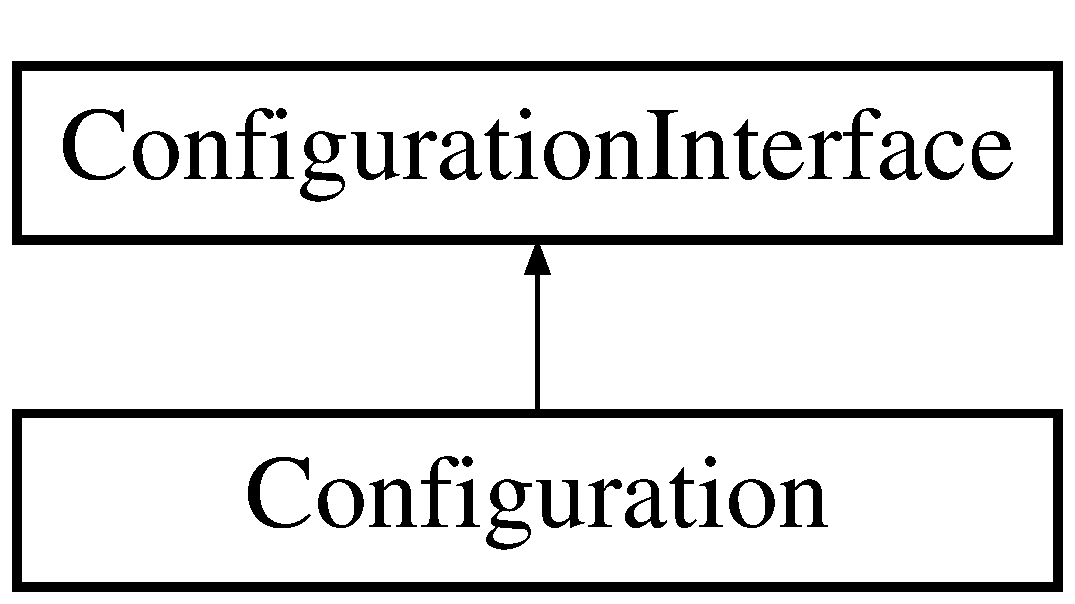
\includegraphics[height=2.000000cm]{class_c_r_1_1_g_s_b_r_bundle_1_1_dependency_injection_1_1_configuration}
\end{center}
\end{figure}
\subsection*{Public Member Functions}
\begin{DoxyCompactItemize}
\item 
{\bf get\+Config\+Tree\+Builder} ()
\end{DoxyCompactItemize}


\subsection{Detailed Description}
This is the class that validates and merges configuration from your app/config files

To learn more see \doxyref{http\+://symfony.\+com/doc/current/cookbook/bundles/extension.\+html\#cookbook-\/bundles-\/extension-\/config-\/class}{p.}{} 

\subsection{Member Function Documentation}
\index{C\+R\+::\+G\+S\+B\+R\+Bundle\+::\+Dependency\+Injection\+::\+Configuration@{C\+R\+::\+G\+S\+B\+R\+Bundle\+::\+Dependency\+Injection\+::\+Configuration}!get\+Config\+Tree\+Builder@{get\+Config\+Tree\+Builder}}
\index{get\+Config\+Tree\+Builder@{get\+Config\+Tree\+Builder}!C\+R\+::\+G\+S\+B\+R\+Bundle\+::\+Dependency\+Injection\+::\+Configuration@{C\+R\+::\+G\+S\+B\+R\+Bundle\+::\+Dependency\+Injection\+::\+Configuration}}
\subsubsection[{get\+Config\+Tree\+Builder}]{\setlength{\rightskip}{0pt plus 5cm}get\+Config\+Tree\+Builder (
\begin{DoxyParamCaption}
{}
\end{DoxyParamCaption}
)}\label{class_c_r_1_1_g_s_b_r_bundle_1_1_dependency_injection_1_1_configuration_ae03f0be384bdd90669c1872f4eb95aff}
\{\} 

The documentation for this class was generated from the following file\+:\begin{DoxyCompactItemize}
\item 
X\+A\+M\+P\+P/xamppfiles/htdocs/\+C\+R/src/\+C\+R/\+G\+S\+B\+R\+Bundle/\+Dependency\+Injection/Configuration.\+php\end{DoxyCompactItemize}

\section{C\+R\+G\+S\+B\+R\+Bundle Class Reference}
\label{class_c_r_1_1_g_s_b_r_bundle_1_1_c_r_g_s_b_r_bundle}\index{C\+R\+G\+S\+B\+R\+Bundle@{C\+R\+G\+S\+B\+R\+Bundle}}
Inheritance diagram for C\+R\+G\+S\+B\+R\+Bundle\+:\begin{figure}[H]
\begin{center}
\leavevmode
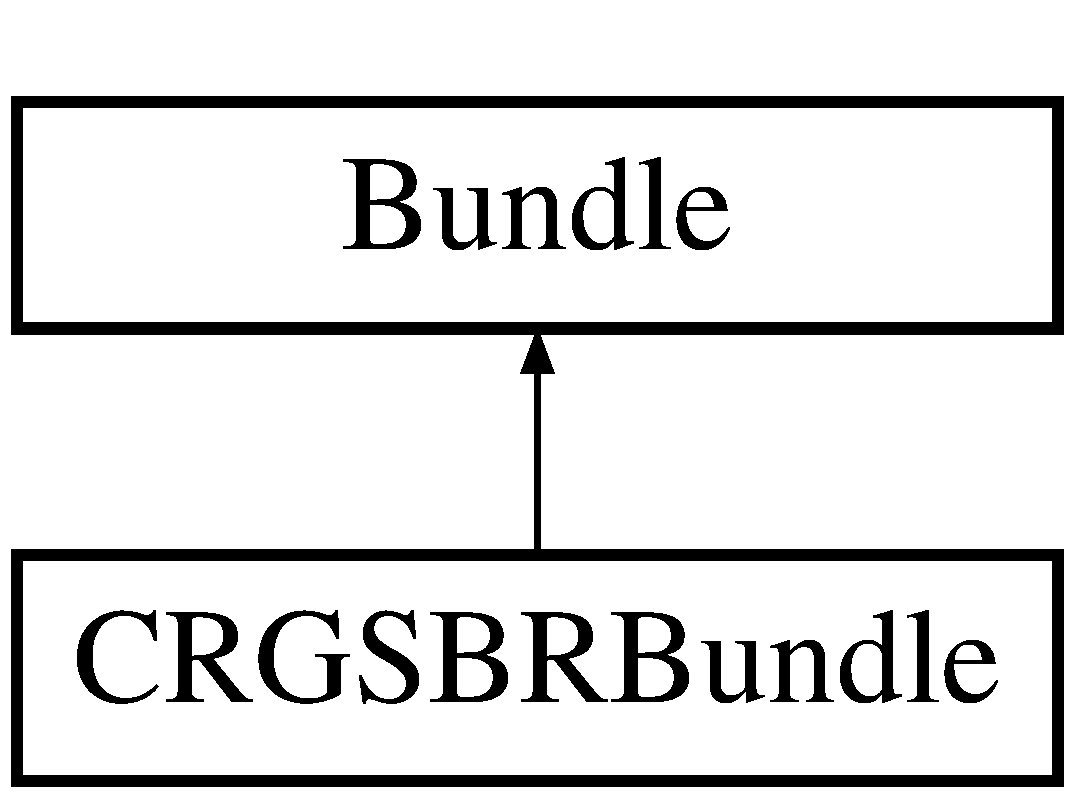
\includegraphics[height=2.000000cm]{class_c_r_1_1_g_s_b_r_bundle_1_1_c_r_g_s_b_r_bundle}
\end{center}
\end{figure}


The documentation for this class was generated from the following file\+:\begin{DoxyCompactItemize}
\item 
X\+A\+M\+P\+P/xamppfiles/htdocs/\+C\+R/src/\+C\+R/\+G\+S\+B\+R\+Bundle/C\+R\+G\+S\+B\+R\+Bundle.\+php\end{DoxyCompactItemize}

\section{C\+R\+G\+S\+B\+R\+Extension Class Reference}
\label{class_c_r_1_1_g_s_b_r_bundle_1_1_dependency_injection_1_1_c_r_g_s_b_r_extension}\index{C\+R\+G\+S\+B\+R\+Extension@{C\+R\+G\+S\+B\+R\+Extension}}
Inheritance diagram for C\+R\+G\+S\+B\+R\+Extension\+:\begin{figure}[H]
\begin{center}
\leavevmode
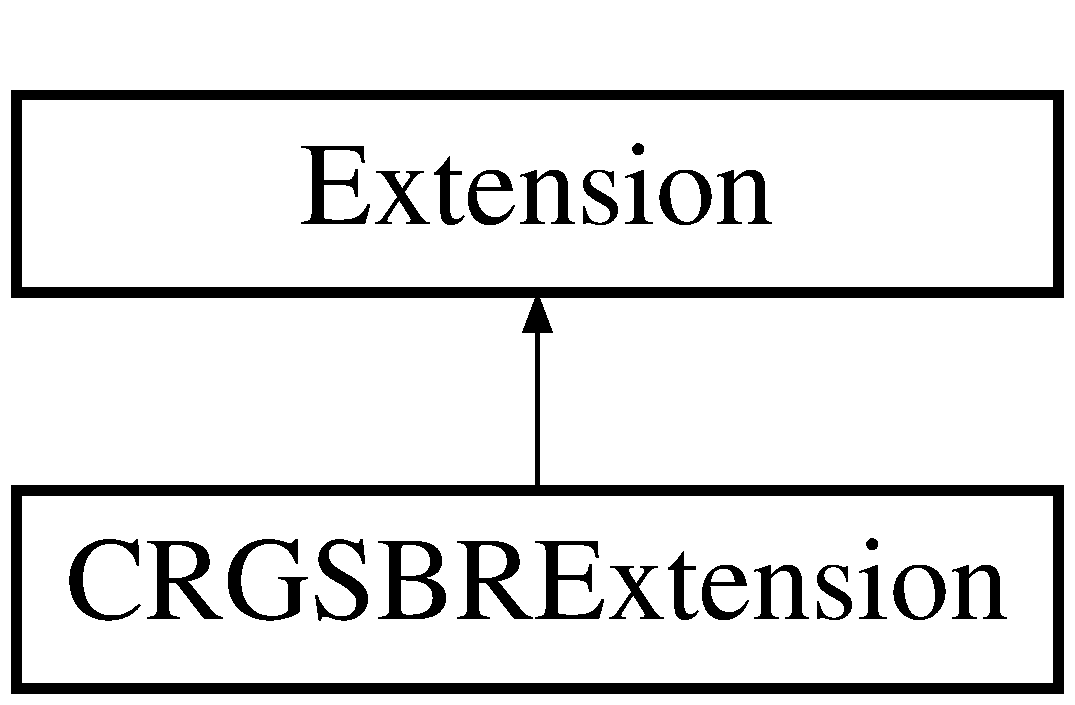
\includegraphics[height=2.000000cm]{class_c_r_1_1_g_s_b_r_bundle_1_1_dependency_injection_1_1_c_r_g_s_b_r_extension}
\end{center}
\end{figure}
\subsection*{Public Member Functions}
\begin{DoxyCompactItemize}
\item 
{\bf load} (array \$configs, Container\+Builder \$container)
\end{DoxyCompactItemize}


\subsection{Detailed Description}
This is the class that loads and manages your bundle configuration

To learn more see \doxyref{http\+://symfony.\+com/doc/current/cookbook/bundles/extension.\+html}{p.}{} 

\subsection{Member Function Documentation}
\index{C\+R\+::\+G\+S\+B\+R\+Bundle\+::\+Dependency\+Injection\+::\+C\+R\+G\+S\+B\+R\+Extension@{C\+R\+::\+G\+S\+B\+R\+Bundle\+::\+Dependency\+Injection\+::\+C\+R\+G\+S\+B\+R\+Extension}!load@{load}}
\index{load@{load}!C\+R\+::\+G\+S\+B\+R\+Bundle\+::\+Dependency\+Injection\+::\+C\+R\+G\+S\+B\+R\+Extension@{C\+R\+::\+G\+S\+B\+R\+Bundle\+::\+Dependency\+Injection\+::\+C\+R\+G\+S\+B\+R\+Extension}}
\subsubsection[{load}]{\setlength{\rightskip}{0pt plus 5cm}load (
\begin{DoxyParamCaption}
\item[{array}]{\$configs, }
\item[{Container\+Builder}]{\$container}
\end{DoxyParamCaption}
)}\label{class_c_r_1_1_g_s_b_r_bundle_1_1_dependency_injection_1_1_c_r_g_s_b_r_extension_a9e89ba4c9793088dc3050305084f79a2}
\{\} 

The documentation for this class was generated from the following file\+:\begin{DoxyCompactItemize}
\item 
X\+A\+M\+P\+P/xamppfiles/htdocs/\+C\+R/src/\+C\+R/\+G\+S\+B\+R\+Bundle/\+Dependency\+Injection/C\+R\+G\+S\+B\+R\+Extension.\+php\end{DoxyCompactItemize}

\section{Default\+Controller\+Test Class Reference}
\label{class_c_r_1_1_g_s_b_r_bundle_1_1_tests_1_1_controller_1_1_default_controller_test}\index{Default\+Controller\+Test@{Default\+Controller\+Test}}
Inheritance diagram for Default\+Controller\+Test\+:\begin{figure}[H]
\begin{center}
\leavevmode
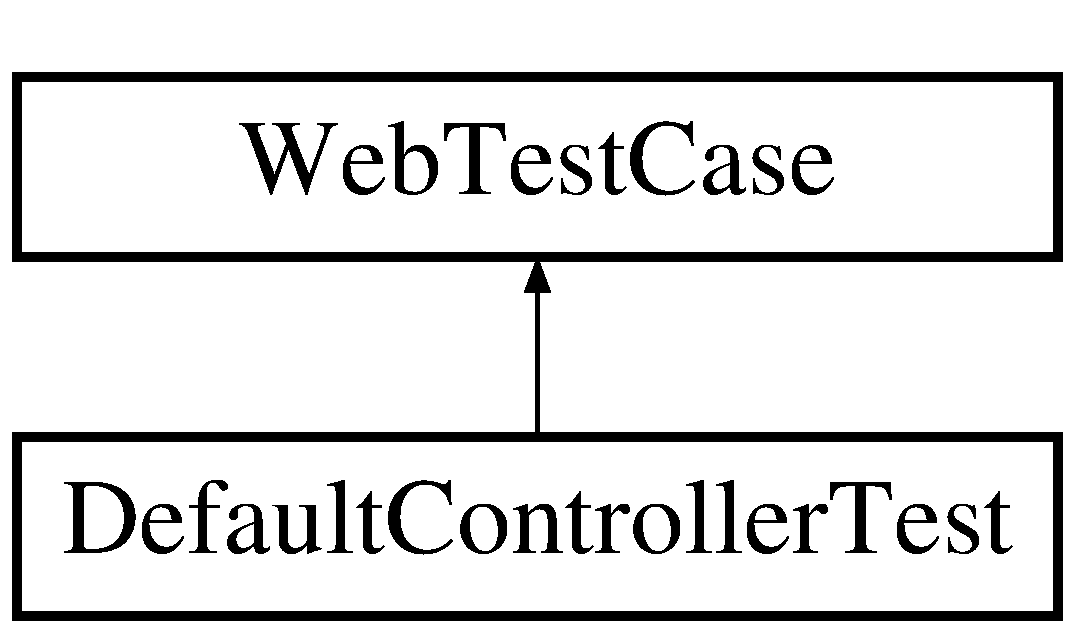
\includegraphics[height=2.000000cm]{class_c_r_1_1_g_s_b_r_bundle_1_1_tests_1_1_controller_1_1_default_controller_test}
\end{center}
\end{figure}
\subsection*{Public Member Functions}
\begin{DoxyCompactItemize}
\item 
{\bfseries test\+Index} ()\label{class_c_r_1_1_g_s_b_r_bundle_1_1_tests_1_1_controller_1_1_default_controller_test_a0d5e64d219e7d25c074c5d022306dd9f}

\end{DoxyCompactItemize}


The documentation for this class was generated from the following file\+:\begin{DoxyCompactItemize}
\item 
X\+A\+M\+P\+P/xamppfiles/htdocs/\+C\+R/src/\+C\+R/\+G\+S\+B\+R\+Bundle/\+Tests/\+Controller/Default\+Controller\+Test.\+php\end{DoxyCompactItemize}

\section{famille Class Reference}
\label{class_c_r_1_1_g_s_b_r_bundle_1_1_entity_1_1famille}\index{famille@{famille}}
\subsection*{Public Member Functions}
\begin{DoxyCompactItemize}
\item 
{\bf get\+Id} ()
\item 
{\bf set\+Libelle\+Famille} (\$libelle\+Famille)
\item 
{\bf get\+Libelle\+Famille} ()
\end{DoxyCompactItemize}


\subsection{Detailed Description}
famille

() (repository\+Class=\char`\"{}\+C\+R\textbackslash{}\+G\+S\+B\+R\+Bundle\textbackslash{}\+Entity\textbackslash{}famille\+Repository\char`\"{}) 

\subsection{Member Function Documentation}
\index{C\+R\+::\+G\+S\+B\+R\+Bundle\+::\+Entity\+::famille@{C\+R\+::\+G\+S\+B\+R\+Bundle\+::\+Entity\+::famille}!get\+Id@{get\+Id}}
\index{get\+Id@{get\+Id}!C\+R\+::\+G\+S\+B\+R\+Bundle\+::\+Entity\+::famille@{C\+R\+::\+G\+S\+B\+R\+Bundle\+::\+Entity\+::famille}}
\subsubsection[{get\+Id}]{\setlength{\rightskip}{0pt plus 5cm}get\+Id (
\begin{DoxyParamCaption}
{}
\end{DoxyParamCaption}
)}\label{class_c_r_1_1_g_s_b_r_bundle_1_1_entity_1_1famille_a12251d0c022e9e21c137a105ff683f13}
Get id

\begin{DoxyReturn}{Returns}
integer 
\end{DoxyReturn}
\index{C\+R\+::\+G\+S\+B\+R\+Bundle\+::\+Entity\+::famille@{C\+R\+::\+G\+S\+B\+R\+Bundle\+::\+Entity\+::famille}!get\+Libelle\+Famille@{get\+Libelle\+Famille}}
\index{get\+Libelle\+Famille@{get\+Libelle\+Famille}!C\+R\+::\+G\+S\+B\+R\+Bundle\+::\+Entity\+::famille@{C\+R\+::\+G\+S\+B\+R\+Bundle\+::\+Entity\+::famille}}
\subsubsection[{get\+Libelle\+Famille}]{\setlength{\rightskip}{0pt plus 5cm}get\+Libelle\+Famille (
\begin{DoxyParamCaption}
{}
\end{DoxyParamCaption}
)}\label{class_c_r_1_1_g_s_b_r_bundle_1_1_entity_1_1famille_afad83dbe78c0283084b7d8a3e905e59e}
Get libelle\+Famille

\begin{DoxyReturn}{Returns}
string 
\end{DoxyReturn}
\index{C\+R\+::\+G\+S\+B\+R\+Bundle\+::\+Entity\+::famille@{C\+R\+::\+G\+S\+B\+R\+Bundle\+::\+Entity\+::famille}!set\+Libelle\+Famille@{set\+Libelle\+Famille}}
\index{set\+Libelle\+Famille@{set\+Libelle\+Famille}!C\+R\+::\+G\+S\+B\+R\+Bundle\+::\+Entity\+::famille@{C\+R\+::\+G\+S\+B\+R\+Bundle\+::\+Entity\+::famille}}
\subsubsection[{set\+Libelle\+Famille}]{\setlength{\rightskip}{0pt plus 5cm}set\+Libelle\+Famille (
\begin{DoxyParamCaption}
\item[{}]{\$libelle\+Famille}
\end{DoxyParamCaption}
)}\label{class_c_r_1_1_g_s_b_r_bundle_1_1_entity_1_1famille_a085efc4420825a298d47f48692331272}
Set libelle\+Famille


\begin{DoxyParams}[1]{Parameters}
string & {\em \$libelle\+Famille} & \\
\hline
\end{DoxyParams}
\begin{DoxyReturn}{Returns}
famille 
\end{DoxyReturn}


The documentation for this class was generated from the following file\+:\begin{DoxyCompactItemize}
\item 
X\+A\+M\+P\+P/xamppfiles/htdocs/\+C\+R/src/\+C\+R/\+G\+S\+B\+R\+Bundle/\+Entity/famille.\+php\end{DoxyCompactItemize}

\section{famille\+Repository Class Reference}
\label{class_c_r_1_1_g_s_b_r_bundle_1_1_entity_1_1famille_repository}\index{famille\+Repository@{famille\+Repository}}
Inheritance diagram for famille\+Repository\+:\begin{figure}[H]
\begin{center}
\leavevmode
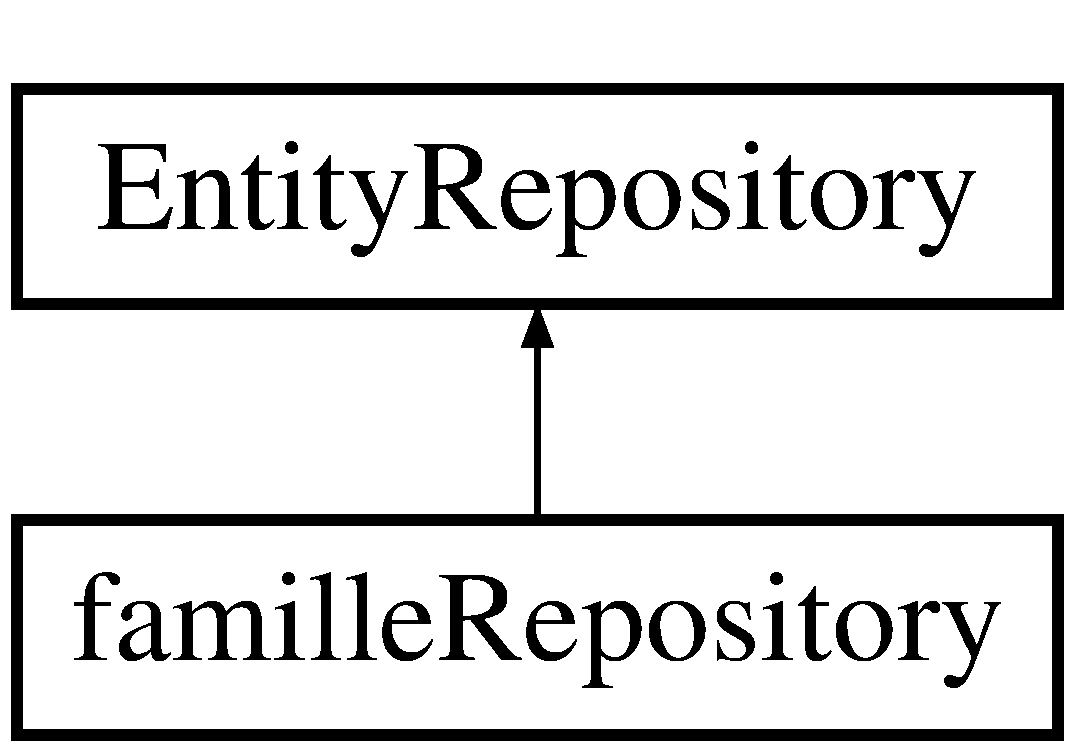
\includegraphics[height=2.000000cm]{class_c_r_1_1_g_s_b_r_bundle_1_1_entity_1_1famille_repository}
\end{center}
\end{figure}


\subsection{Detailed Description}
\doxyref{famille\+Repository}{p.}{class_c_r_1_1_g_s_b_r_bundle_1_1_entity_1_1famille_repository}

This class was generated by the Doctrine O\+R\+M. Add your own custom repository methods below. 

The documentation for this class was generated from the following file\+:\begin{DoxyCompactItemize}
\item 
X\+A\+M\+P\+P/xamppfiles/htdocs/\+C\+R/src/\+C\+R/\+G\+S\+B\+R\+Bundle/\+Entity/famille\+Repository.\+php\end{DoxyCompactItemize}

\section{Home\+Controller Class Reference}
\label{class_c_r_1_1_g_s_b_r_bundle_1_1_controller_1_1_home_controller}\index{Home\+Controller@{Home\+Controller}}
Inheritance diagram for Home\+Controller\+:\begin{figure}[H]
\begin{center}
\leavevmode
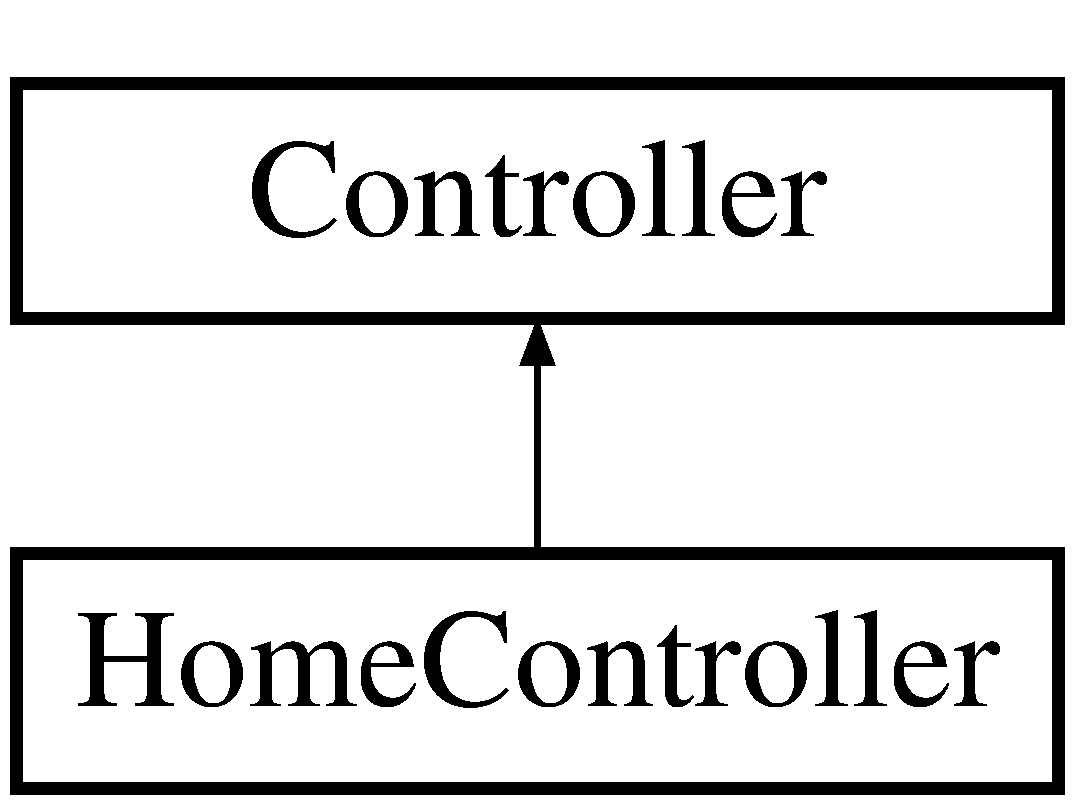
\includegraphics[height=2.000000cm]{class_c_r_1_1_g_s_b_r_bundle_1_1_controller_1_1_home_controller}
\end{center}
\end{figure}
\subsection*{Public Member Functions}
\begin{DoxyCompactItemize}
\item 
{\bf index\+Action} ()
\item 
{\bf login\+Action} ()
\item 
{\bf profil\+Action} (Request \$request)
\end{DoxyCompactItemize}


\subsection{Detailed Description}
Classe contrôleur d\textquotesingle{}accès à l\textquotesingle{}application et de gestion du profil 

\subsection{Member Function Documentation}
\index{C\+R\+::\+G\+S\+B\+R\+Bundle\+::\+Controller\+::\+Home\+Controller@{C\+R\+::\+G\+S\+B\+R\+Bundle\+::\+Controller\+::\+Home\+Controller}!index\+Action@{index\+Action}}
\index{index\+Action@{index\+Action}!C\+R\+::\+G\+S\+B\+R\+Bundle\+::\+Controller\+::\+Home\+Controller@{C\+R\+::\+G\+S\+B\+R\+Bundle\+::\+Controller\+::\+Home\+Controller}}
\subsubsection[{index\+Action}]{\setlength{\rightskip}{0pt plus 5cm}index\+Action (
\begin{DoxyParamCaption}
{}
\end{DoxyParamCaption}
)}\label{class_c_r_1_1_g_s_b_r_bundle_1_1_controller_1_1_home_controller_a04f2101fe1cdc785b61219c2df753024}
Cette fonction affiche la page d\textquotesingle{}accueil \begin{DoxyReturn}{Returns}
view Retourne la vue accueil.\+html.\+twig 
\end{DoxyReturn}
\index{C\+R\+::\+G\+S\+B\+R\+Bundle\+::\+Controller\+::\+Home\+Controller@{C\+R\+::\+G\+S\+B\+R\+Bundle\+::\+Controller\+::\+Home\+Controller}!login\+Action@{login\+Action}}
\index{login\+Action@{login\+Action}!C\+R\+::\+G\+S\+B\+R\+Bundle\+::\+Controller\+::\+Home\+Controller@{C\+R\+::\+G\+S\+B\+R\+Bundle\+::\+Controller\+::\+Home\+Controller}}
\subsubsection[{login\+Action}]{\setlength{\rightskip}{0pt plus 5cm}login\+Action (
\begin{DoxyParamCaption}
{}
\end{DoxyParamCaption}
)}\label{class_c_r_1_1_g_s_b_r_bundle_1_1_controller_1_1_home_controller_ae29767bbd6584fd74defa4a888972c72}
Cette fonction gère la connexion à l\textquotesingle{}application \begin{DoxyReturn}{Returns}
view Retourne la vue connexion.\+html.\+twig 
\end{DoxyReturn}
\index{C\+R\+::\+G\+S\+B\+R\+Bundle\+::\+Controller\+::\+Home\+Controller@{C\+R\+::\+G\+S\+B\+R\+Bundle\+::\+Controller\+::\+Home\+Controller}!profil\+Action@{profil\+Action}}
\index{profil\+Action@{profil\+Action}!C\+R\+::\+G\+S\+B\+R\+Bundle\+::\+Controller\+::\+Home\+Controller@{C\+R\+::\+G\+S\+B\+R\+Bundle\+::\+Controller\+::\+Home\+Controller}}
\subsubsection[{profil\+Action}]{\setlength{\rightskip}{0pt plus 5cm}profil\+Action (
\begin{DoxyParamCaption}
\item[{Request}]{\$request}
\end{DoxyParamCaption}
)}\label{class_c_r_1_1_g_s_b_r_bundle_1_1_controller_1_1_home_controller_a7afbe219d4156b67af1c76ed716103a0}
Cette fonction affiche la page du formulaire du profil \begin{DoxyReturn}{Returns}
view Retourne la vue profil.\+html.\+twig 
\end{DoxyReturn}


The documentation for this class was generated from the following file\+:\begin{DoxyCompactItemize}
\item 
X\+A\+M\+P\+P/xamppfiles/htdocs/\+C\+R/src/\+C\+R/\+G\+S\+B\+R\+Bundle/\+Controller/Home\+Controller.\+php\end{DoxyCompactItemize}

\section{medicament Class Reference}
\label{class_c_r_1_1_g_s_b_r_bundle_1_1_entity_1_1medicament}\index{medicament@{medicament}}
\subsection*{Public Member Functions}
\begin{DoxyCompactItemize}
\item 
{\bf get\+Id} ()
\item 
{\bf set\+Depot\+Legal} (\$depot\+Legal)
\item 
{\bf get\+Depot\+Legal} ()
\item 
{\bf set\+Nom\+Commercial} (\$nom\+Commercial)
\item 
{\bf get\+Nom\+Commercial} ()
\item 
{\bf set\+Composition} (\$composition)
\item 
{\bf get\+Composition} ()
\item 
{\bf set\+Effets} (\$effets)
\item 
{\bf get\+Effets} ()
\item 
{\bf set\+Contre\+Indication} (\$contre\+Indication)
\item 
{\bf get\+Contre\+Indication} ()
\item 
{\bf set\+Prix\+Echantillon} (\$prix\+Echantillon)
\item 
{\bf get\+Prix\+Echantillon} ()
\item 
{\bf set\+Famille} (\textbackslash{}{\bf C\+R\textbackslash{}\+G\+S\+B\+R\+Bundle\textbackslash{}\+Entity\textbackslash{}famille} \${\bf famille}=null)
\item 
{\bf get\+Famille} ()
\end{DoxyCompactItemize}


\subsection{Detailed Description}
medicament

() (repository\+Class=\char`\"{}\+C\+R\textbackslash{}\+G\+S\+B\+R\+Bundle\textbackslash{}\+Entity\textbackslash{}medicament\+Repository\char`\"{}) 

\subsection{Member Function Documentation}
\index{C\+R\+::\+G\+S\+B\+R\+Bundle\+::\+Entity\+::medicament@{C\+R\+::\+G\+S\+B\+R\+Bundle\+::\+Entity\+::medicament}!get\+Composition@{get\+Composition}}
\index{get\+Composition@{get\+Composition}!C\+R\+::\+G\+S\+B\+R\+Bundle\+::\+Entity\+::medicament@{C\+R\+::\+G\+S\+B\+R\+Bundle\+::\+Entity\+::medicament}}
\subsubsection[{get\+Composition}]{\setlength{\rightskip}{0pt plus 5cm}get\+Composition (
\begin{DoxyParamCaption}
{}
\end{DoxyParamCaption}
)}\label{class_c_r_1_1_g_s_b_r_bundle_1_1_entity_1_1medicament_ac1fbb5f7c107966f8f1df97ec6e7aacb}
Get composition

\begin{DoxyReturn}{Returns}
string 
\end{DoxyReturn}
\index{C\+R\+::\+G\+S\+B\+R\+Bundle\+::\+Entity\+::medicament@{C\+R\+::\+G\+S\+B\+R\+Bundle\+::\+Entity\+::medicament}!get\+Contre\+Indication@{get\+Contre\+Indication}}
\index{get\+Contre\+Indication@{get\+Contre\+Indication}!C\+R\+::\+G\+S\+B\+R\+Bundle\+::\+Entity\+::medicament@{C\+R\+::\+G\+S\+B\+R\+Bundle\+::\+Entity\+::medicament}}
\subsubsection[{get\+Contre\+Indication}]{\setlength{\rightskip}{0pt plus 5cm}get\+Contre\+Indication (
\begin{DoxyParamCaption}
{}
\end{DoxyParamCaption}
)}\label{class_c_r_1_1_g_s_b_r_bundle_1_1_entity_1_1medicament_a21cf7250d8f140d2f1800b5f3a70ab6d}
Get contre\+Indication

\begin{DoxyReturn}{Returns}
string 
\end{DoxyReturn}
\index{C\+R\+::\+G\+S\+B\+R\+Bundle\+::\+Entity\+::medicament@{C\+R\+::\+G\+S\+B\+R\+Bundle\+::\+Entity\+::medicament}!get\+Depot\+Legal@{get\+Depot\+Legal}}
\index{get\+Depot\+Legal@{get\+Depot\+Legal}!C\+R\+::\+G\+S\+B\+R\+Bundle\+::\+Entity\+::medicament@{C\+R\+::\+G\+S\+B\+R\+Bundle\+::\+Entity\+::medicament}}
\subsubsection[{get\+Depot\+Legal}]{\setlength{\rightskip}{0pt plus 5cm}get\+Depot\+Legal (
\begin{DoxyParamCaption}
{}
\end{DoxyParamCaption}
)}\label{class_c_r_1_1_g_s_b_r_bundle_1_1_entity_1_1medicament_a42ec65ea7e62656a4de900a1d105a727}
Get depot\+Legal

\begin{DoxyReturn}{Returns}
string 
\end{DoxyReturn}
\index{C\+R\+::\+G\+S\+B\+R\+Bundle\+::\+Entity\+::medicament@{C\+R\+::\+G\+S\+B\+R\+Bundle\+::\+Entity\+::medicament}!get\+Effets@{get\+Effets}}
\index{get\+Effets@{get\+Effets}!C\+R\+::\+G\+S\+B\+R\+Bundle\+::\+Entity\+::medicament@{C\+R\+::\+G\+S\+B\+R\+Bundle\+::\+Entity\+::medicament}}
\subsubsection[{get\+Effets}]{\setlength{\rightskip}{0pt plus 5cm}get\+Effets (
\begin{DoxyParamCaption}
{}
\end{DoxyParamCaption}
)}\label{class_c_r_1_1_g_s_b_r_bundle_1_1_entity_1_1medicament_aaad3ec1237b3218e540f0da854f0debf}
Get effets

\begin{DoxyReturn}{Returns}
string 
\end{DoxyReturn}
\index{C\+R\+::\+G\+S\+B\+R\+Bundle\+::\+Entity\+::medicament@{C\+R\+::\+G\+S\+B\+R\+Bundle\+::\+Entity\+::medicament}!get\+Famille@{get\+Famille}}
\index{get\+Famille@{get\+Famille}!C\+R\+::\+G\+S\+B\+R\+Bundle\+::\+Entity\+::medicament@{C\+R\+::\+G\+S\+B\+R\+Bundle\+::\+Entity\+::medicament}}
\subsubsection[{get\+Famille}]{\setlength{\rightskip}{0pt plus 5cm}get\+Famille (
\begin{DoxyParamCaption}
{}
\end{DoxyParamCaption}
)}\label{class_c_r_1_1_g_s_b_r_bundle_1_1_entity_1_1medicament_a58482364aa1e470a1fda8ec8ff7d3fdf}
Get famille

\begin{DoxyReturn}{Returns}

\end{DoxyReturn}
\index{C\+R\+::\+G\+S\+B\+R\+Bundle\+::\+Entity\+::medicament@{C\+R\+::\+G\+S\+B\+R\+Bundle\+::\+Entity\+::medicament}!get\+Id@{get\+Id}}
\index{get\+Id@{get\+Id}!C\+R\+::\+G\+S\+B\+R\+Bundle\+::\+Entity\+::medicament@{C\+R\+::\+G\+S\+B\+R\+Bundle\+::\+Entity\+::medicament}}
\subsubsection[{get\+Id}]{\setlength{\rightskip}{0pt plus 5cm}get\+Id (
\begin{DoxyParamCaption}
{}
\end{DoxyParamCaption}
)}\label{class_c_r_1_1_g_s_b_r_bundle_1_1_entity_1_1medicament_a12251d0c022e9e21c137a105ff683f13}
Get id

\begin{DoxyReturn}{Returns}
integer 
\end{DoxyReturn}
\index{C\+R\+::\+G\+S\+B\+R\+Bundle\+::\+Entity\+::medicament@{C\+R\+::\+G\+S\+B\+R\+Bundle\+::\+Entity\+::medicament}!get\+Nom\+Commercial@{get\+Nom\+Commercial}}
\index{get\+Nom\+Commercial@{get\+Nom\+Commercial}!C\+R\+::\+G\+S\+B\+R\+Bundle\+::\+Entity\+::medicament@{C\+R\+::\+G\+S\+B\+R\+Bundle\+::\+Entity\+::medicament}}
\subsubsection[{get\+Nom\+Commercial}]{\setlength{\rightskip}{0pt plus 5cm}get\+Nom\+Commercial (
\begin{DoxyParamCaption}
{}
\end{DoxyParamCaption}
)}\label{class_c_r_1_1_g_s_b_r_bundle_1_1_entity_1_1medicament_a25ac56fb8d7ceb863c7551ebeaac6166}
Get nom\+Commercial

\begin{DoxyReturn}{Returns}
string 
\end{DoxyReturn}
\index{C\+R\+::\+G\+S\+B\+R\+Bundle\+::\+Entity\+::medicament@{C\+R\+::\+G\+S\+B\+R\+Bundle\+::\+Entity\+::medicament}!get\+Prix\+Echantillon@{get\+Prix\+Echantillon}}
\index{get\+Prix\+Echantillon@{get\+Prix\+Echantillon}!C\+R\+::\+G\+S\+B\+R\+Bundle\+::\+Entity\+::medicament@{C\+R\+::\+G\+S\+B\+R\+Bundle\+::\+Entity\+::medicament}}
\subsubsection[{get\+Prix\+Echantillon}]{\setlength{\rightskip}{0pt plus 5cm}get\+Prix\+Echantillon (
\begin{DoxyParamCaption}
{}
\end{DoxyParamCaption}
)}\label{class_c_r_1_1_g_s_b_r_bundle_1_1_entity_1_1medicament_abb31f3d827cae12e08c8de935d680b65}
Get prix\+Echantillon

\begin{DoxyReturn}{Returns}
float 
\end{DoxyReturn}
\index{C\+R\+::\+G\+S\+B\+R\+Bundle\+::\+Entity\+::medicament@{C\+R\+::\+G\+S\+B\+R\+Bundle\+::\+Entity\+::medicament}!set\+Composition@{set\+Composition}}
\index{set\+Composition@{set\+Composition}!C\+R\+::\+G\+S\+B\+R\+Bundle\+::\+Entity\+::medicament@{C\+R\+::\+G\+S\+B\+R\+Bundle\+::\+Entity\+::medicament}}
\subsubsection[{set\+Composition}]{\setlength{\rightskip}{0pt plus 5cm}set\+Composition (
\begin{DoxyParamCaption}
\item[{}]{\$composition}
\end{DoxyParamCaption}
)}\label{class_c_r_1_1_g_s_b_r_bundle_1_1_entity_1_1medicament_a878d2b8ea3342526423eccd446ca3115}
Set composition


\begin{DoxyParams}[1]{Parameters}
string & {\em \$composition} & \\
\hline
\end{DoxyParams}
\begin{DoxyReturn}{Returns}
medicament 
\end{DoxyReturn}
\index{C\+R\+::\+G\+S\+B\+R\+Bundle\+::\+Entity\+::medicament@{C\+R\+::\+G\+S\+B\+R\+Bundle\+::\+Entity\+::medicament}!set\+Contre\+Indication@{set\+Contre\+Indication}}
\index{set\+Contre\+Indication@{set\+Contre\+Indication}!C\+R\+::\+G\+S\+B\+R\+Bundle\+::\+Entity\+::medicament@{C\+R\+::\+G\+S\+B\+R\+Bundle\+::\+Entity\+::medicament}}
\subsubsection[{set\+Contre\+Indication}]{\setlength{\rightskip}{0pt plus 5cm}set\+Contre\+Indication (
\begin{DoxyParamCaption}
\item[{}]{\$contre\+Indication}
\end{DoxyParamCaption}
)}\label{class_c_r_1_1_g_s_b_r_bundle_1_1_entity_1_1medicament_ad1a5ca3765d6266b5ae706eabbd1ff2b}
Set contre\+Indication


\begin{DoxyParams}[1]{Parameters}
string & {\em \$contre\+Indication} & \\
\hline
\end{DoxyParams}
\begin{DoxyReturn}{Returns}
medicament 
\end{DoxyReturn}
\index{C\+R\+::\+G\+S\+B\+R\+Bundle\+::\+Entity\+::medicament@{C\+R\+::\+G\+S\+B\+R\+Bundle\+::\+Entity\+::medicament}!set\+Depot\+Legal@{set\+Depot\+Legal}}
\index{set\+Depot\+Legal@{set\+Depot\+Legal}!C\+R\+::\+G\+S\+B\+R\+Bundle\+::\+Entity\+::medicament@{C\+R\+::\+G\+S\+B\+R\+Bundle\+::\+Entity\+::medicament}}
\subsubsection[{set\+Depot\+Legal}]{\setlength{\rightskip}{0pt plus 5cm}set\+Depot\+Legal (
\begin{DoxyParamCaption}
\item[{}]{\$depot\+Legal}
\end{DoxyParamCaption}
)}\label{class_c_r_1_1_g_s_b_r_bundle_1_1_entity_1_1medicament_a9a638639799a1989c5ac68cdd5e0c109}
Set depot\+Legal


\begin{DoxyParams}[1]{Parameters}
string & {\em \$depot\+Legal} & \\
\hline
\end{DoxyParams}
\begin{DoxyReturn}{Returns}
medicament 
\end{DoxyReturn}
\index{C\+R\+::\+G\+S\+B\+R\+Bundle\+::\+Entity\+::medicament@{C\+R\+::\+G\+S\+B\+R\+Bundle\+::\+Entity\+::medicament}!set\+Effets@{set\+Effets}}
\index{set\+Effets@{set\+Effets}!C\+R\+::\+G\+S\+B\+R\+Bundle\+::\+Entity\+::medicament@{C\+R\+::\+G\+S\+B\+R\+Bundle\+::\+Entity\+::medicament}}
\subsubsection[{set\+Effets}]{\setlength{\rightskip}{0pt plus 5cm}set\+Effets (
\begin{DoxyParamCaption}
\item[{}]{\$effets}
\end{DoxyParamCaption}
)}\label{class_c_r_1_1_g_s_b_r_bundle_1_1_entity_1_1medicament_adde84115849de05166b9ee912edb932b}
Set effets


\begin{DoxyParams}[1]{Parameters}
string & {\em \$effets} & \\
\hline
\end{DoxyParams}
\begin{DoxyReturn}{Returns}
medicament 
\end{DoxyReturn}
\index{C\+R\+::\+G\+S\+B\+R\+Bundle\+::\+Entity\+::medicament@{C\+R\+::\+G\+S\+B\+R\+Bundle\+::\+Entity\+::medicament}!set\+Famille@{set\+Famille}}
\index{set\+Famille@{set\+Famille}!C\+R\+::\+G\+S\+B\+R\+Bundle\+::\+Entity\+::medicament@{C\+R\+::\+G\+S\+B\+R\+Bundle\+::\+Entity\+::medicament}}
\subsubsection[{set\+Famille}]{\setlength{\rightskip}{0pt plus 5cm}set\+Famille (
\begin{DoxyParamCaption}
\item[{\textbackslash{}{\bf C\+R\textbackslash{}\+G\+S\+B\+R\+Bundle\textbackslash{}\+Entity\textbackslash{}famille}}]{\$famille = {\ttfamily null}}
\end{DoxyParamCaption}
)}\label{class_c_r_1_1_g_s_b_r_bundle_1_1_entity_1_1medicament_a8eb50092deb32a609f779c730279f620}
Set famille


\begin{DoxyParams}[1]{Parameters}
\textbackslash{}\+C\+R\textbackslash{}\+G\+S\+B\+R\+Bundle\textbackslash{}\+Entity\textbackslash{}famille & {\em \$famille} & \\
\hline
\end{DoxyParams}
\begin{DoxyReturn}{Returns}
medicament 
\end{DoxyReturn}
\index{C\+R\+::\+G\+S\+B\+R\+Bundle\+::\+Entity\+::medicament@{C\+R\+::\+G\+S\+B\+R\+Bundle\+::\+Entity\+::medicament}!set\+Nom\+Commercial@{set\+Nom\+Commercial}}
\index{set\+Nom\+Commercial@{set\+Nom\+Commercial}!C\+R\+::\+G\+S\+B\+R\+Bundle\+::\+Entity\+::medicament@{C\+R\+::\+G\+S\+B\+R\+Bundle\+::\+Entity\+::medicament}}
\subsubsection[{set\+Nom\+Commercial}]{\setlength{\rightskip}{0pt plus 5cm}set\+Nom\+Commercial (
\begin{DoxyParamCaption}
\item[{}]{\$nom\+Commercial}
\end{DoxyParamCaption}
)}\label{class_c_r_1_1_g_s_b_r_bundle_1_1_entity_1_1medicament_ab09c38fc078240024d346208502e2356}
Set nom\+Commercial


\begin{DoxyParams}[1]{Parameters}
string & {\em \$nom\+Commercial} & \\
\hline
\end{DoxyParams}
\begin{DoxyReturn}{Returns}
medicament 
\end{DoxyReturn}
\index{C\+R\+::\+G\+S\+B\+R\+Bundle\+::\+Entity\+::medicament@{C\+R\+::\+G\+S\+B\+R\+Bundle\+::\+Entity\+::medicament}!set\+Prix\+Echantillon@{set\+Prix\+Echantillon}}
\index{set\+Prix\+Echantillon@{set\+Prix\+Echantillon}!C\+R\+::\+G\+S\+B\+R\+Bundle\+::\+Entity\+::medicament@{C\+R\+::\+G\+S\+B\+R\+Bundle\+::\+Entity\+::medicament}}
\subsubsection[{set\+Prix\+Echantillon}]{\setlength{\rightskip}{0pt plus 5cm}set\+Prix\+Echantillon (
\begin{DoxyParamCaption}
\item[{}]{\$prix\+Echantillon}
\end{DoxyParamCaption}
)}\label{class_c_r_1_1_g_s_b_r_bundle_1_1_entity_1_1medicament_a92d2143e6c469cdb6fdc38922bab2cff}
Set prix\+Echantillon


\begin{DoxyParams}[1]{Parameters}
float & {\em \$prix\+Echantillon} & \\
\hline
\end{DoxyParams}
\begin{DoxyReturn}{Returns}
medicament 
\end{DoxyReturn}


The documentation for this class was generated from the following file\+:\begin{DoxyCompactItemize}
\item 
X\+A\+M\+P\+P/xamppfiles/htdocs/\+C\+R/src/\+C\+R/\+G\+S\+B\+R\+Bundle/\+Entity/medicament.\+php\end{DoxyCompactItemize}

\section{Medicament\+Controller Class Reference}
\label{class_c_r_1_1_g_s_b_r_bundle_1_1_controller_1_1_medicament_controller}\index{Medicament\+Controller@{Medicament\+Controller}}
Inheritance diagram for Medicament\+Controller\+:\begin{figure}[H]
\begin{center}
\leavevmode
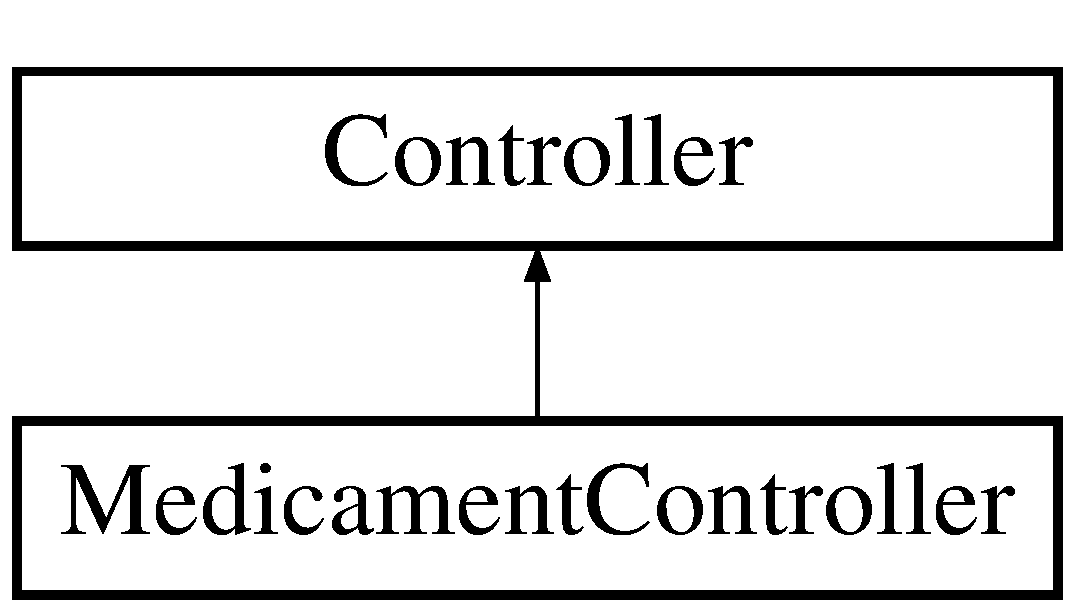
\includegraphics[height=2.000000cm]{class_c_r_1_1_g_s_b_r_bundle_1_1_controller_1_1_medicament_controller}
\end{center}
\end{figure}
\subsection*{Public Member Functions}
\begin{DoxyCompactItemize}
\item 
{\bf index\+Action} ()
\item 
{\bf recherche\+Action} ()
\item 
{\bf resultat\+Action} (Request \$request)
\end{DoxyCompactItemize}


\subsection{Detailed Description}
Classe contrôleur de consultation et recherche des médicaments 

\subsection{Member Function Documentation}
\index{C\+R\+::\+G\+S\+B\+R\+Bundle\+::\+Controller\+::\+Medicament\+Controller@{C\+R\+::\+G\+S\+B\+R\+Bundle\+::\+Controller\+::\+Medicament\+Controller}!index\+Action@{index\+Action}}
\index{index\+Action@{index\+Action}!C\+R\+::\+G\+S\+B\+R\+Bundle\+::\+Controller\+::\+Medicament\+Controller@{C\+R\+::\+G\+S\+B\+R\+Bundle\+::\+Controller\+::\+Medicament\+Controller}}
\subsubsection[{index\+Action}]{\setlength{\rightskip}{0pt plus 5cm}index\+Action (
\begin{DoxyParamCaption}
{}
\end{DoxyParamCaption}
)}\label{class_c_r_1_1_g_s_b_r_bundle_1_1_controller_1_1_medicament_controller_a04f2101fe1cdc785b61219c2df753024}
Cette fonction affiche la page /medicament/ \begin{DoxyReturn}{Returns}
view Retourne la vue medicament.\+html.\+twig 
\end{DoxyReturn}
\index{C\+R\+::\+G\+S\+B\+R\+Bundle\+::\+Controller\+::\+Medicament\+Controller@{C\+R\+::\+G\+S\+B\+R\+Bundle\+::\+Controller\+::\+Medicament\+Controller}!recherche\+Action@{recherche\+Action}}
\index{recherche\+Action@{recherche\+Action}!C\+R\+::\+G\+S\+B\+R\+Bundle\+::\+Controller\+::\+Medicament\+Controller@{C\+R\+::\+G\+S\+B\+R\+Bundle\+::\+Controller\+::\+Medicament\+Controller}}
\subsubsection[{recherche\+Action}]{\setlength{\rightskip}{0pt plus 5cm}recherche\+Action (
\begin{DoxyParamCaption}
{}
\end{DoxyParamCaption}
)}\label{class_c_r_1_1_g_s_b_r_bundle_1_1_controller_1_1_medicament_controller_afc5ebc9e38bd370740b7bce95f708232}
Cette fonction recherche l\textquotesingle{}ensemble des familles \begin{DoxyReturn}{Returns}
array \$les\+Familles Les familles de médicaments 
\end{DoxyReturn}
\index{C\+R\+::\+G\+S\+B\+R\+Bundle\+::\+Controller\+::\+Medicament\+Controller@{C\+R\+::\+G\+S\+B\+R\+Bundle\+::\+Controller\+::\+Medicament\+Controller}!resultat\+Action@{resultat\+Action}}
\index{resultat\+Action@{resultat\+Action}!C\+R\+::\+G\+S\+B\+R\+Bundle\+::\+Controller\+::\+Medicament\+Controller@{C\+R\+::\+G\+S\+B\+R\+Bundle\+::\+Controller\+::\+Medicament\+Controller}}
\subsubsection[{resultat\+Action}]{\setlength{\rightskip}{0pt plus 5cm}resultat\+Action (
\begin{DoxyParamCaption}
\item[{Request}]{\$request}
\end{DoxyParamCaption}
)}\label{class_c_r_1_1_g_s_b_r_bundle_1_1_controller_1_1_medicament_controller_a815e9d79cde937c21578a068a15e888f}
Cette fonction retourne le résultat de la recherche de médicament


\begin{DoxyParams}[1]{Parameters}
Request & {\em \$request} & La requête construite à partir de la séléction de l\textquotesingle{}utilisateur \\
\hline
\end{DoxyParams}
\begin{DoxyReturn}{Returns}
view recherche\+Medicament.\+html.\+twig la vue avec le résultat 
\end{DoxyReturn}
récupère toutes les familles de médicaments de la B\+D\+D 

The documentation for this class was generated from the following file\+:\begin{DoxyCompactItemize}
\item 
X\+A\+M\+P\+P/xamppfiles/htdocs/\+C\+R/src/\+C\+R/\+G\+S\+B\+R\+Bundle/\+Controller/Medicament\+Controller.\+php\end{DoxyCompactItemize}

\section{medicament\+Repository Class Reference}
\label{class_c_r_1_1_g_s_b_r_bundle_1_1_entity_1_1medicament_repository}\index{medicament\+Repository@{medicament\+Repository}}
Inheritance diagram for medicament\+Repository\+:\begin{figure}[H]
\begin{center}
\leavevmode
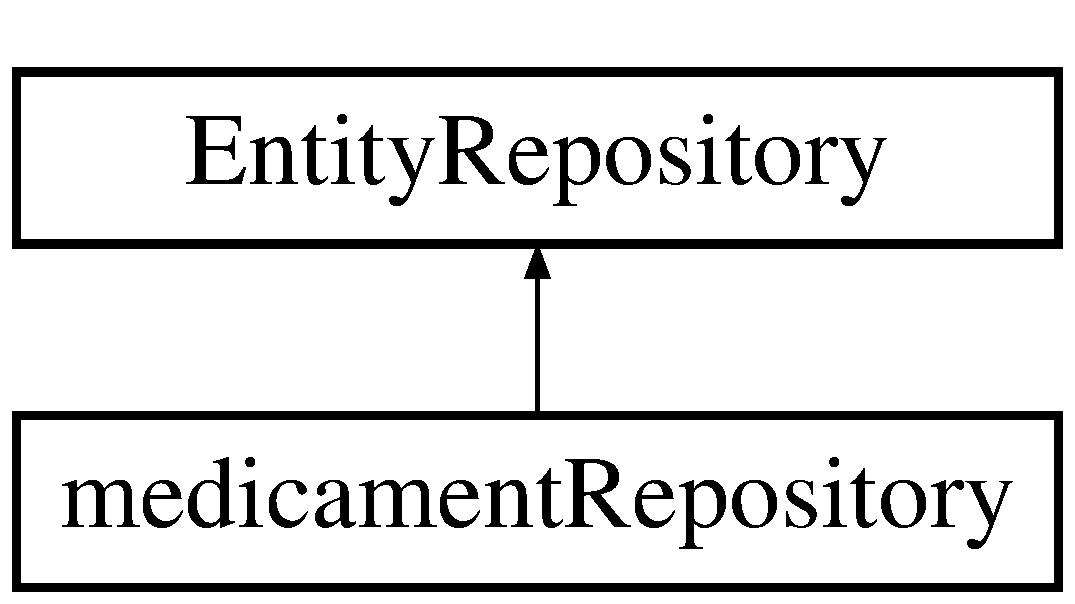
\includegraphics[height=2.000000cm]{class_c_r_1_1_g_s_b_r_bundle_1_1_entity_1_1medicament_repository}
\end{center}
\end{figure}
\subsection*{Public Member Functions}
\begin{DoxyCompactItemize}
\item 
{\bfseries find\+All} ()\label{class_c_r_1_1_g_s_b_r_bundle_1_1_entity_1_1medicament_repository_a73a1b0348919b6755e4f69dcc70eba64}

\end{DoxyCompactItemize}


\subsection{Detailed Description}
\doxyref{medicament\+Repository}{p.}{class_c_r_1_1_g_s_b_r_bundle_1_1_entity_1_1medicament_repository}

This class was generated by the Doctrine O\+R\+M. Add your own custom repository methods below. 

The documentation for this class was generated from the following file\+:\begin{DoxyCompactItemize}
\item 
X\+A\+M\+P\+P/xamppfiles/htdocs/\+C\+R/src/\+C\+R/\+G\+S\+B\+R\+Bundle/\+Entity/medicament\+Repository.\+php\end{DoxyCompactItemize}

\section{Pdo\+Gsb Class Reference}
\label{class_c_r_1_1_g_s_b_r_bundle_1_1services_1_1_pdo_gsb}\index{Pdo\+Gsb@{Pdo\+Gsb}}
\subsection*{Public Member Functions}
\begin{DoxyCompactItemize}
\item 
{\bf \+\_\+\+\_\+construct} (\$serveur, \$bdd, \$user, \$mdp)
\item 
{\bfseries \+\_\+destruct} ()\label{class_c_r_1_1_g_s_b_r_bundle_1_1services_1_1_pdo_gsb_a1c6024f681d3956654622d9f28e540a2}

\item 
{\bf get\+Infos\+Visiteur} (\$login, \$mdp)
\item 
{\bf get\+Les\+Frais\+Hors\+Forfait} (\$id\+Visiteur, \$mois)
\item 
{\bf get\+Nbjustificatifs} (\$id\+Visiteur, \$mois)
\item 
{\bf get\+Les\+Frais\+Forfait} (\$id\+Visiteur, \$mois)
\item 
{\bf get\+Les\+Id\+Frais} ()
\item 
{\bf maj\+Frais\+Forfait} (\$id\+Visiteur, \$mois, \$les\+Frais)
\item 
{\bf maj\+Nb\+Justificatifs} (\$id\+Visiteur, \$mois, \$nb\+Justificatifs)
\item 
{\bf est\+Premier\+Frais\+Mois} (\$id\+Visiteur, \$mois)
\item 
{\bf dernier\+Mois\+Saisi} (\$id\+Visiteur)
\item 
{\bf cree\+Nouvelles\+Lignes\+Frais} (\$id\+Visiteur, \$mois)
\item 
{\bf cree\+Nouveau\+Frais\+Hors\+Forfait} (\$id\+Visiteur, \$mois, \$libelle, \$date, \$montant)
\item 
{\bf supprimer\+Frais\+Hors\+Forfait} (\$id\+Frais)
\item 
{\bf get\+Les\+Mois\+Disponibles} (\$id\+Visiteur)
\item 
{\bf get\+Les\+Infos\+Fiche\+Frais} (\$id\+Visiteur, \$mois)
\item 
{\bf maj\+Etat\+Fiche\+Frais} (\$id\+Visiteur, \$mois, \$etat)
\item 
{\bf get\+Les\+Fiches\+Validees} ()
\item 
{\bf est\+Valide\+Suppression\+Frais} (\$id\+Visiteur, \$mois, \$id\+Frais)
\end{DoxyCompactItemize}
\subsection*{Static Public Member Functions}
\begin{DoxyCompactItemize}
\item 
static {\bf get\+Pdo\+Gsb} ()
\end{DoxyCompactItemize}


\subsection{Constructor \& Destructor Documentation}
\index{C\+R\+::\+G\+S\+B\+R\+Bundle\+::services\+::\+Pdo\+Gsb@{C\+R\+::\+G\+S\+B\+R\+Bundle\+::services\+::\+Pdo\+Gsb}!\+\_\+\+\_\+construct@{\+\_\+\+\_\+construct}}
\index{\+\_\+\+\_\+construct@{\+\_\+\+\_\+construct}!C\+R\+::\+G\+S\+B\+R\+Bundle\+::services\+::\+Pdo\+Gsb@{C\+R\+::\+G\+S\+B\+R\+Bundle\+::services\+::\+Pdo\+Gsb}}
\subsubsection[{\+\_\+\+\_\+construct}]{\setlength{\rightskip}{0pt plus 5cm}\+\_\+\+\_\+construct (
\begin{DoxyParamCaption}
\item[{}]{\$serveur, }
\item[{}]{\$bdd, }
\item[{}]{\$user, }
\item[{}]{\$mdp}
\end{DoxyParamCaption}
)}\label{class_c_r_1_1_g_s_b_r_bundle_1_1services_1_1_pdo_gsb_ac8081b766b24c3a67106613003efdbd6}
Constructeur privé, crée l\textquotesingle{}instance de P\+D\+O qui sera sollicitée pour toutes les méthodes de la classe 

\subsection{Member Function Documentation}
\index{C\+R\+::\+G\+S\+B\+R\+Bundle\+::services\+::\+Pdo\+Gsb@{C\+R\+::\+G\+S\+B\+R\+Bundle\+::services\+::\+Pdo\+Gsb}!cree\+Nouveau\+Frais\+Hors\+Forfait@{cree\+Nouveau\+Frais\+Hors\+Forfait}}
\index{cree\+Nouveau\+Frais\+Hors\+Forfait@{cree\+Nouveau\+Frais\+Hors\+Forfait}!C\+R\+::\+G\+S\+B\+R\+Bundle\+::services\+::\+Pdo\+Gsb@{C\+R\+::\+G\+S\+B\+R\+Bundle\+::services\+::\+Pdo\+Gsb}}
\subsubsection[{cree\+Nouveau\+Frais\+Hors\+Forfait}]{\setlength{\rightskip}{0pt plus 5cm}cree\+Nouveau\+Frais\+Hors\+Forfait (
\begin{DoxyParamCaption}
\item[{}]{\$id\+Visiteur, }
\item[{}]{\$mois, }
\item[{}]{\$libelle, }
\item[{}]{\$date, }
\item[{}]{\$montant}
\end{DoxyParamCaption}
)}\label{class_c_r_1_1_g_s_b_r_bundle_1_1services_1_1_pdo_gsb_a5b4ae76bd318baa9ee6d57f53b43d1d8}
Crée un nouveau frais hors forfait pour un visiteur un mois donné à partir des informations fournies en paramètre


\begin{DoxyParams}{Parameters}
{\em \$id\+Visiteur} & \\
\hline
{\em \$mois} & sous la forme aaaamm \\
\hline
{\em \$libelle} & \+: le libelle du frais \\
\hline
{\em \$date} & \+: la date du frais au format français jj//mm/aaaa \\
\hline
{\em \$montant} & \+: le montant \\
\hline
\end{DoxyParams}
\index{C\+R\+::\+G\+S\+B\+R\+Bundle\+::services\+::\+Pdo\+Gsb@{C\+R\+::\+G\+S\+B\+R\+Bundle\+::services\+::\+Pdo\+Gsb}!cree\+Nouvelles\+Lignes\+Frais@{cree\+Nouvelles\+Lignes\+Frais}}
\index{cree\+Nouvelles\+Lignes\+Frais@{cree\+Nouvelles\+Lignes\+Frais}!C\+R\+::\+G\+S\+B\+R\+Bundle\+::services\+::\+Pdo\+Gsb@{C\+R\+::\+G\+S\+B\+R\+Bundle\+::services\+::\+Pdo\+Gsb}}
\subsubsection[{cree\+Nouvelles\+Lignes\+Frais}]{\setlength{\rightskip}{0pt plus 5cm}cree\+Nouvelles\+Lignes\+Frais (
\begin{DoxyParamCaption}
\item[{}]{\$id\+Visiteur, }
\item[{}]{\$mois}
\end{DoxyParamCaption}
)}\label{class_c_r_1_1_g_s_b_r_bundle_1_1services_1_1_pdo_gsb_ae42a666f0c62b60a6fe35448e3600d8a}
Crée une nouvelle fiche de frais et les lignes de frais au forfait pour un visiteur et un mois donnés

récupère le dernier mois en cours de traitement, met à \textquotesingle{}C\+L\textquotesingle{} son champs id\+Etat, crée une nouvelle fiche de frais avec un id\+Etat à \textquotesingle{}C\+R\textquotesingle{} et crée les lignes de frais forfait de quantités nulles 
\begin{DoxyParams}{Parameters}
{\em \$id\+Visiteur} & \\
\hline
{\em \$mois} & sous la forme aaaamm \\
\hline
\end{DoxyParams}
\index{C\+R\+::\+G\+S\+B\+R\+Bundle\+::services\+::\+Pdo\+Gsb@{C\+R\+::\+G\+S\+B\+R\+Bundle\+::services\+::\+Pdo\+Gsb}!dernier\+Mois\+Saisi@{dernier\+Mois\+Saisi}}
\index{dernier\+Mois\+Saisi@{dernier\+Mois\+Saisi}!C\+R\+::\+G\+S\+B\+R\+Bundle\+::services\+::\+Pdo\+Gsb@{C\+R\+::\+G\+S\+B\+R\+Bundle\+::services\+::\+Pdo\+Gsb}}
\subsubsection[{dernier\+Mois\+Saisi}]{\setlength{\rightskip}{0pt plus 5cm}dernier\+Mois\+Saisi (
\begin{DoxyParamCaption}
\item[{}]{\$id\+Visiteur}
\end{DoxyParamCaption}
)}\label{class_c_r_1_1_g_s_b_r_bundle_1_1services_1_1_pdo_gsb_a5bde16f5acfa92c7810433187f3e05f1}
Retourne le dernier mois en cours d\textquotesingle{}un visiteur


\begin{DoxyParams}{Parameters}
{\em \$id\+Visiteur} & \\
\hline
\end{DoxyParams}
\begin{DoxyReturn}{Returns}
le mois sous la forme aaaamm 
\end{DoxyReturn}
\index{C\+R\+::\+G\+S\+B\+R\+Bundle\+::services\+::\+Pdo\+Gsb@{C\+R\+::\+G\+S\+B\+R\+Bundle\+::services\+::\+Pdo\+Gsb}!est\+Premier\+Frais\+Mois@{est\+Premier\+Frais\+Mois}}
\index{est\+Premier\+Frais\+Mois@{est\+Premier\+Frais\+Mois}!C\+R\+::\+G\+S\+B\+R\+Bundle\+::services\+::\+Pdo\+Gsb@{C\+R\+::\+G\+S\+B\+R\+Bundle\+::services\+::\+Pdo\+Gsb}}
\subsubsection[{est\+Premier\+Frais\+Mois}]{\setlength{\rightskip}{0pt plus 5cm}est\+Premier\+Frais\+Mois (
\begin{DoxyParamCaption}
\item[{}]{\$id\+Visiteur, }
\item[{}]{\$mois}
\end{DoxyParamCaption}
)}\label{class_c_r_1_1_g_s_b_r_bundle_1_1services_1_1_pdo_gsb_a426147406c706370eeb5d17175c33562}
Teste si un visiteur possède une fiche de frais pour le mois passé en argument


\begin{DoxyParams}{Parameters}
{\em \$id\+Visiteur} & \\
\hline
{\em \$mois} & sous la forme aaaamm \\
\hline
\end{DoxyParams}
\begin{DoxyReturn}{Returns}
vrai ou faux 
\end{DoxyReturn}
\index{C\+R\+::\+G\+S\+B\+R\+Bundle\+::services\+::\+Pdo\+Gsb@{C\+R\+::\+G\+S\+B\+R\+Bundle\+::services\+::\+Pdo\+Gsb}!est\+Valide\+Suppression\+Frais@{est\+Valide\+Suppression\+Frais}}
\index{est\+Valide\+Suppression\+Frais@{est\+Valide\+Suppression\+Frais}!C\+R\+::\+G\+S\+B\+R\+Bundle\+::services\+::\+Pdo\+Gsb@{C\+R\+::\+G\+S\+B\+R\+Bundle\+::services\+::\+Pdo\+Gsb}}
\subsubsection[{est\+Valide\+Suppression\+Frais}]{\setlength{\rightskip}{0pt plus 5cm}est\+Valide\+Suppression\+Frais (
\begin{DoxyParamCaption}
\item[{}]{\$id\+Visiteur, }
\item[{}]{\$mois, }
\item[{}]{\$id\+Frais}
\end{DoxyParamCaption}
)}\label{class_c_r_1_1_g_s_b_r_bundle_1_1services_1_1_pdo_gsb_ac30e43ee3dc62720ea0fe266713182ae}
Vérifie si un frais existe pour un visiteur et un mois donné 
\begin{DoxyParams}[1]{Parameters}
type & {\em \$id\+Visiteur} & \\
\hline
type & {\em \$mois} & \\
\hline
type & {\em \$id\+Frais} & \\
\hline
\end{DoxyParams}
\begin{DoxyReturn}{Returns}
1 ou 0 
\end{DoxyReturn}
\index{C\+R\+::\+G\+S\+B\+R\+Bundle\+::services\+::\+Pdo\+Gsb@{C\+R\+::\+G\+S\+B\+R\+Bundle\+::services\+::\+Pdo\+Gsb}!get\+Infos\+Visiteur@{get\+Infos\+Visiteur}}
\index{get\+Infos\+Visiteur@{get\+Infos\+Visiteur}!C\+R\+::\+G\+S\+B\+R\+Bundle\+::services\+::\+Pdo\+Gsb@{C\+R\+::\+G\+S\+B\+R\+Bundle\+::services\+::\+Pdo\+Gsb}}
\subsubsection[{get\+Infos\+Visiteur}]{\setlength{\rightskip}{0pt plus 5cm}get\+Infos\+Visiteur (
\begin{DoxyParamCaption}
\item[{}]{\$login, }
\item[{}]{\$mdp}
\end{DoxyParamCaption}
)}\label{class_c_r_1_1_g_s_b_r_bundle_1_1services_1_1_pdo_gsb_a3405f494d610cddab3b7dcfb2fe80d45}
Retourne les informations d\textquotesingle{}un visiteur


\begin{DoxyParams}{Parameters}
{\em \$login} & \\
\hline
{\em \$mdp} & \\
\hline
\end{DoxyParams}
\begin{DoxyReturn}{Returns}
l\textquotesingle{}id, le nom et le prénom sous la forme d\textquotesingle{}un tableau associatif 
\end{DoxyReturn}
\index{C\+R\+::\+G\+S\+B\+R\+Bundle\+::services\+::\+Pdo\+Gsb@{C\+R\+::\+G\+S\+B\+R\+Bundle\+::services\+::\+Pdo\+Gsb}!get\+Les\+Fiches\+Validees@{get\+Les\+Fiches\+Validees}}
\index{get\+Les\+Fiches\+Validees@{get\+Les\+Fiches\+Validees}!C\+R\+::\+G\+S\+B\+R\+Bundle\+::services\+::\+Pdo\+Gsb@{C\+R\+::\+G\+S\+B\+R\+Bundle\+::services\+::\+Pdo\+Gsb}}
\subsubsection[{get\+Les\+Fiches\+Validees}]{\setlength{\rightskip}{0pt plus 5cm}get\+Les\+Fiches\+Validees (
\begin{DoxyParamCaption}
{}
\end{DoxyParamCaption}
)}\label{class_c_r_1_1_g_s_b_r_bundle_1_1services_1_1_pdo_gsb_a10f3e2899f7bd0a3c837bf6d2b480ffa}
Retourne toutes les fiches de frais dont l\textquotesingle{}état est à validé \begin{DoxyReturn}{Returns}
type 
\end{DoxyReturn}
\index{C\+R\+::\+G\+S\+B\+R\+Bundle\+::services\+::\+Pdo\+Gsb@{C\+R\+::\+G\+S\+B\+R\+Bundle\+::services\+::\+Pdo\+Gsb}!get\+Les\+Frais\+Forfait@{get\+Les\+Frais\+Forfait}}
\index{get\+Les\+Frais\+Forfait@{get\+Les\+Frais\+Forfait}!C\+R\+::\+G\+S\+B\+R\+Bundle\+::services\+::\+Pdo\+Gsb@{C\+R\+::\+G\+S\+B\+R\+Bundle\+::services\+::\+Pdo\+Gsb}}
\subsubsection[{get\+Les\+Frais\+Forfait}]{\setlength{\rightskip}{0pt plus 5cm}get\+Les\+Frais\+Forfait (
\begin{DoxyParamCaption}
\item[{}]{\$id\+Visiteur, }
\item[{}]{\$mois}
\end{DoxyParamCaption}
)}\label{class_c_r_1_1_g_s_b_r_bundle_1_1services_1_1_pdo_gsb_a5792eb474723cda0a758735f5fbb791e}
Retourne sous forme d\textquotesingle{}un tableau associatif toutes les lignes de frais au forfait concernées par les deux arguments


\begin{DoxyParams}{Parameters}
{\em \$id\+Visiteur} & \\
\hline
{\em \$mois} & sous la forme aaaamm \\
\hline
\end{DoxyParams}
\begin{DoxyReturn}{Returns}
l\textquotesingle{}id, le libelle et la quantité sous la forme d\textquotesingle{}un tableau associatif 
\end{DoxyReturn}
\index{C\+R\+::\+G\+S\+B\+R\+Bundle\+::services\+::\+Pdo\+Gsb@{C\+R\+::\+G\+S\+B\+R\+Bundle\+::services\+::\+Pdo\+Gsb}!get\+Les\+Frais\+Hors\+Forfait@{get\+Les\+Frais\+Hors\+Forfait}}
\index{get\+Les\+Frais\+Hors\+Forfait@{get\+Les\+Frais\+Hors\+Forfait}!C\+R\+::\+G\+S\+B\+R\+Bundle\+::services\+::\+Pdo\+Gsb@{C\+R\+::\+G\+S\+B\+R\+Bundle\+::services\+::\+Pdo\+Gsb}}
\subsubsection[{get\+Les\+Frais\+Hors\+Forfait}]{\setlength{\rightskip}{0pt plus 5cm}get\+Les\+Frais\+Hors\+Forfait (
\begin{DoxyParamCaption}
\item[{}]{\$id\+Visiteur, }
\item[{}]{\$mois}
\end{DoxyParamCaption}
)}\label{class_c_r_1_1_g_s_b_r_bundle_1_1services_1_1_pdo_gsb_aa89782786e0037745abd9c62b25ade20}
Retourne sous forme d\textquotesingle{}un tableau associatif toutes les lignes de frais hors forfait concernées par les deux arguments

La boucle foreach ne peut être utilisée ici car on procède à une modification de la structure itérée -\/ transformation du champ date-\/


\begin{DoxyParams}{Parameters}
{\em \$id\+Visiteur} & \\
\hline
{\em \$mois} & sous la forme aaaamm \\
\hline
\end{DoxyParams}
\begin{DoxyReturn}{Returns}
tous les champs des lignes de frais hors forfait sous la forme d\textquotesingle{}un tableau associatif 
\end{DoxyReturn}
\index{C\+R\+::\+G\+S\+B\+R\+Bundle\+::services\+::\+Pdo\+Gsb@{C\+R\+::\+G\+S\+B\+R\+Bundle\+::services\+::\+Pdo\+Gsb}!get\+Les\+Id\+Frais@{get\+Les\+Id\+Frais}}
\index{get\+Les\+Id\+Frais@{get\+Les\+Id\+Frais}!C\+R\+::\+G\+S\+B\+R\+Bundle\+::services\+::\+Pdo\+Gsb@{C\+R\+::\+G\+S\+B\+R\+Bundle\+::services\+::\+Pdo\+Gsb}}
\subsubsection[{get\+Les\+Id\+Frais}]{\setlength{\rightskip}{0pt plus 5cm}get\+Les\+Id\+Frais (
\begin{DoxyParamCaption}
{}
\end{DoxyParamCaption}
)}\label{class_c_r_1_1_g_s_b_r_bundle_1_1services_1_1_pdo_gsb_ad0943d4cabc4e6bfd803ecab13be0e57}
Retourne tous les id de la table Frais\+Forfait

\begin{DoxyReturn}{Returns}
un tableau associatif 
\end{DoxyReturn}
\index{C\+R\+::\+G\+S\+B\+R\+Bundle\+::services\+::\+Pdo\+Gsb@{C\+R\+::\+G\+S\+B\+R\+Bundle\+::services\+::\+Pdo\+Gsb}!get\+Les\+Infos\+Fiche\+Frais@{get\+Les\+Infos\+Fiche\+Frais}}
\index{get\+Les\+Infos\+Fiche\+Frais@{get\+Les\+Infos\+Fiche\+Frais}!C\+R\+::\+G\+S\+B\+R\+Bundle\+::services\+::\+Pdo\+Gsb@{C\+R\+::\+G\+S\+B\+R\+Bundle\+::services\+::\+Pdo\+Gsb}}
\subsubsection[{get\+Les\+Infos\+Fiche\+Frais}]{\setlength{\rightskip}{0pt plus 5cm}get\+Les\+Infos\+Fiche\+Frais (
\begin{DoxyParamCaption}
\item[{}]{\$id\+Visiteur, }
\item[{}]{\$mois}
\end{DoxyParamCaption}
)}\label{class_c_r_1_1_g_s_b_r_bundle_1_1services_1_1_pdo_gsb_af243a6fda5669151cd4d35c66bcd13a4}
Retourne les informations d\textquotesingle{}une fiche de frais d\textquotesingle{}un visiteur pour un mois donné


\begin{DoxyParams}{Parameters}
{\em \$id\+Visiteur} & \\
\hline
{\em \$mois} & sous la forme aaaamm \\
\hline
\end{DoxyParams}
\begin{DoxyReturn}{Returns}
un tableau avec des champs de jointure entre une fiche de frais et la ligne d\textquotesingle{}état 
\end{DoxyReturn}
\index{C\+R\+::\+G\+S\+B\+R\+Bundle\+::services\+::\+Pdo\+Gsb@{C\+R\+::\+G\+S\+B\+R\+Bundle\+::services\+::\+Pdo\+Gsb}!get\+Les\+Mois\+Disponibles@{get\+Les\+Mois\+Disponibles}}
\index{get\+Les\+Mois\+Disponibles@{get\+Les\+Mois\+Disponibles}!C\+R\+::\+G\+S\+B\+R\+Bundle\+::services\+::\+Pdo\+Gsb@{C\+R\+::\+G\+S\+B\+R\+Bundle\+::services\+::\+Pdo\+Gsb}}
\subsubsection[{get\+Les\+Mois\+Disponibles}]{\setlength{\rightskip}{0pt plus 5cm}get\+Les\+Mois\+Disponibles (
\begin{DoxyParamCaption}
\item[{}]{\$id\+Visiteur}
\end{DoxyParamCaption}
)}\label{class_c_r_1_1_g_s_b_r_bundle_1_1services_1_1_pdo_gsb_a34f4b6a3081514827f3726ac49dcded3}
Retourne les mois pour lesquel un visiteur a une fiche de frais


\begin{DoxyParams}{Parameters}
{\em \$id\+Visiteur} & \\
\hline
\end{DoxyParams}
\begin{DoxyReturn}{Returns}
un tableau associatif de clé un mois -\/aaaamm-\/ et de valeurs l\textquotesingle{}année et le mois correspondant 
\end{DoxyReturn}
\index{C\+R\+::\+G\+S\+B\+R\+Bundle\+::services\+::\+Pdo\+Gsb@{C\+R\+::\+G\+S\+B\+R\+Bundle\+::services\+::\+Pdo\+Gsb}!get\+Nbjustificatifs@{get\+Nbjustificatifs}}
\index{get\+Nbjustificatifs@{get\+Nbjustificatifs}!C\+R\+::\+G\+S\+B\+R\+Bundle\+::services\+::\+Pdo\+Gsb@{C\+R\+::\+G\+S\+B\+R\+Bundle\+::services\+::\+Pdo\+Gsb}}
\subsubsection[{get\+Nbjustificatifs}]{\setlength{\rightskip}{0pt plus 5cm}get\+Nbjustificatifs (
\begin{DoxyParamCaption}
\item[{}]{\$id\+Visiteur, }
\item[{}]{\$mois}
\end{DoxyParamCaption}
)}\label{class_c_r_1_1_g_s_b_r_bundle_1_1services_1_1_pdo_gsb_a147b85ddcddef68c57acf34857630ba7}
Retourne le nombre de justificatif d\textquotesingle{}un visiteur pour un mois donné


\begin{DoxyParams}{Parameters}
{\em \$id\+Visiteur} & \\
\hline
{\em \$mois} & sous la forme aaaamm \\
\hline
\end{DoxyParams}
\begin{DoxyReturn}{Returns}
le nombre entier de justificatifs 
\end{DoxyReturn}
\index{C\+R\+::\+G\+S\+B\+R\+Bundle\+::services\+::\+Pdo\+Gsb@{C\+R\+::\+G\+S\+B\+R\+Bundle\+::services\+::\+Pdo\+Gsb}!get\+Pdo\+Gsb@{get\+Pdo\+Gsb}}
\index{get\+Pdo\+Gsb@{get\+Pdo\+Gsb}!C\+R\+::\+G\+S\+B\+R\+Bundle\+::services\+::\+Pdo\+Gsb@{C\+R\+::\+G\+S\+B\+R\+Bundle\+::services\+::\+Pdo\+Gsb}}
\subsubsection[{get\+Pdo\+Gsb}]{\setlength{\rightskip}{0pt plus 5cm}static get\+Pdo\+Gsb (
\begin{DoxyParamCaption}
{}
\end{DoxyParamCaption}
)\hspace{0.3cm}{\ttfamily [static]}}\label{class_c_r_1_1_g_s_b_r_bundle_1_1services_1_1_pdo_gsb_a37ab3ed998137aeaf4d581365520067e}
Fonction statique qui crée l\textquotesingle{}unique instance de la classe

Appel \+: \$instance\+Pdo\+Gsb = \doxyref{Pdo\+Gsb\+::get\+Pdo\+Gsb()}{p.}{class_c_r_1_1_g_s_b_r_bundle_1_1services_1_1_pdo_gsb_a37ab3ed998137aeaf4d581365520067e};

\begin{DoxyReturn}{Returns}
l\textquotesingle{}unique objet de la classe \doxyref{Pdo\+Gsb}{p.}{class_c_r_1_1_g_s_b_r_bundle_1_1services_1_1_pdo_gsb} 
\end{DoxyReturn}
\index{C\+R\+::\+G\+S\+B\+R\+Bundle\+::services\+::\+Pdo\+Gsb@{C\+R\+::\+G\+S\+B\+R\+Bundle\+::services\+::\+Pdo\+Gsb}!maj\+Etat\+Fiche\+Frais@{maj\+Etat\+Fiche\+Frais}}
\index{maj\+Etat\+Fiche\+Frais@{maj\+Etat\+Fiche\+Frais}!C\+R\+::\+G\+S\+B\+R\+Bundle\+::services\+::\+Pdo\+Gsb@{C\+R\+::\+G\+S\+B\+R\+Bundle\+::services\+::\+Pdo\+Gsb}}
\subsubsection[{maj\+Etat\+Fiche\+Frais}]{\setlength{\rightskip}{0pt plus 5cm}maj\+Etat\+Fiche\+Frais (
\begin{DoxyParamCaption}
\item[{}]{\$id\+Visiteur, }
\item[{}]{\$mois, }
\item[{}]{\$etat}
\end{DoxyParamCaption}
)}\label{class_c_r_1_1_g_s_b_r_bundle_1_1services_1_1_pdo_gsb_a92f294d975e98efcfa1d4c9e08a51bcc}
Modifie l\textquotesingle{}état et la date de modification d\textquotesingle{}une fiche de frais

Modifie le champ id\+Etat et met la date de modif à aujourd\textquotesingle{}hui 
\begin{DoxyParams}{Parameters}
{\em \$id\+Visiteur} & \\
\hline
{\em \$mois} & sous la forme aaaamm \\
\hline
\end{DoxyParams}
\index{C\+R\+::\+G\+S\+B\+R\+Bundle\+::services\+::\+Pdo\+Gsb@{C\+R\+::\+G\+S\+B\+R\+Bundle\+::services\+::\+Pdo\+Gsb}!maj\+Frais\+Forfait@{maj\+Frais\+Forfait}}
\index{maj\+Frais\+Forfait@{maj\+Frais\+Forfait}!C\+R\+::\+G\+S\+B\+R\+Bundle\+::services\+::\+Pdo\+Gsb@{C\+R\+::\+G\+S\+B\+R\+Bundle\+::services\+::\+Pdo\+Gsb}}
\subsubsection[{maj\+Frais\+Forfait}]{\setlength{\rightskip}{0pt plus 5cm}maj\+Frais\+Forfait (
\begin{DoxyParamCaption}
\item[{}]{\$id\+Visiteur, }
\item[{}]{\$mois, }
\item[{}]{\$les\+Frais}
\end{DoxyParamCaption}
)}\label{class_c_r_1_1_g_s_b_r_bundle_1_1services_1_1_pdo_gsb_abeb6aae3e806cd3235ebec6ae5cbe7de}
Met à jour la table ligne\+Frais\+Forfait

Met à jour la table ligne\+Frais\+Forfait pour un visiteur et un mois donné en enregistrant les nouveaux montants


\begin{DoxyParams}{Parameters}
{\em \$id\+Visiteur} & \\
\hline
{\em \$mois} & sous la forme aaaamm \\
\hline
{\em \$les\+Frais} & tableau associatif de clé id\+Frais et de valeur la quantité pour ce frais \\
\hline
\end{DoxyParams}
\begin{DoxyReturn}{Returns}
un tableau associatif 
\end{DoxyReturn}
\index{C\+R\+::\+G\+S\+B\+R\+Bundle\+::services\+::\+Pdo\+Gsb@{C\+R\+::\+G\+S\+B\+R\+Bundle\+::services\+::\+Pdo\+Gsb}!maj\+Nb\+Justificatifs@{maj\+Nb\+Justificatifs}}
\index{maj\+Nb\+Justificatifs@{maj\+Nb\+Justificatifs}!C\+R\+::\+G\+S\+B\+R\+Bundle\+::services\+::\+Pdo\+Gsb@{C\+R\+::\+G\+S\+B\+R\+Bundle\+::services\+::\+Pdo\+Gsb}}
\subsubsection[{maj\+Nb\+Justificatifs}]{\setlength{\rightskip}{0pt plus 5cm}maj\+Nb\+Justificatifs (
\begin{DoxyParamCaption}
\item[{}]{\$id\+Visiteur, }
\item[{}]{\$mois, }
\item[{}]{\$nb\+Justificatifs}
\end{DoxyParamCaption}
)}\label{class_c_r_1_1_g_s_b_r_bundle_1_1services_1_1_pdo_gsb_ac3bcdeeb2e7522120cec7ec068b153b3}
met à jour le nombre de justificatifs de la table fiche\+Frais pour le mois et le visiteur concerné


\begin{DoxyParams}{Parameters}
{\em \$id\+Visiteur} & \\
\hline
{\em \$mois} & sous la forme aaaamm \\
\hline
\end{DoxyParams}
\index{C\+R\+::\+G\+S\+B\+R\+Bundle\+::services\+::\+Pdo\+Gsb@{C\+R\+::\+G\+S\+B\+R\+Bundle\+::services\+::\+Pdo\+Gsb}!supprimer\+Frais\+Hors\+Forfait@{supprimer\+Frais\+Hors\+Forfait}}
\index{supprimer\+Frais\+Hors\+Forfait@{supprimer\+Frais\+Hors\+Forfait}!C\+R\+::\+G\+S\+B\+R\+Bundle\+::services\+::\+Pdo\+Gsb@{C\+R\+::\+G\+S\+B\+R\+Bundle\+::services\+::\+Pdo\+Gsb}}
\subsubsection[{supprimer\+Frais\+Hors\+Forfait}]{\setlength{\rightskip}{0pt plus 5cm}supprimer\+Frais\+Hors\+Forfait (
\begin{DoxyParamCaption}
\item[{}]{\$id\+Frais}
\end{DoxyParamCaption}
)}\label{class_c_r_1_1_g_s_b_r_bundle_1_1services_1_1_pdo_gsb_a8806fa2b12726a88a04845316e7c9586}
Supprime le frais hors forfait dont l\textquotesingle{}id est passé en argument


\begin{DoxyParams}{Parameters}
{\em \$id\+Frais} & \\
\hline
\end{DoxyParams}


The documentation for this class was generated from the following file\+:\begin{DoxyCompactItemize}
\item 
X\+A\+M\+P\+P/xamppfiles/htdocs/\+C\+R/src/\+C\+R/\+G\+S\+B\+R\+Bundle/services/Pdo\+Gsb.\+php\end{DoxyCompactItemize}

\section{praticien Class Reference}
\label{class_c_r_1_1_g_s_b_r_bundle_1_1_entity_1_1praticien}\index{praticien@{praticien}}
\subsection*{Public Member Functions}
\begin{DoxyCompactItemize}
\item 
{\bf get\+Id} ()
\item 
{\bf set\+Nom\+Medecin} (\$nom\+Medecin)
\item 
{\bf get\+Nom\+Medecin} ()
\item 
{\bf set\+Prenom\+Medecin} (\$prenom\+Medecin)
\item 
{\bf get\+Prenom\+Medecin} ()
\item 
{\bf set\+Cp\+Medecin} (\$cp\+Medecin)
\item 
{\bf get\+Cp\+Medecin} ()
\item 
{\bf set\+Ville\+Medecin} (\$ville\+Medecin)
\item 
{\bf get\+Ville\+Medecin} ()
\item 
{\bf set\+Coef\+Notoriete} (\$coef\+Notoriete)
\item 
{\bf get\+Coef\+Notoriete} ()
\item 
{\bf set\+Type\+Medecin} (\textbackslash{}{\bf C\+R\textbackslash{}\+G\+S\+B\+R\+Bundle\textbackslash{}\+Entity\textbackslash{}type\+Praticien} \$type\+Medecin=null)
\item 
{\bf get\+Type\+Medecin} ()
\item 
{\bf set\+Adresse\+Medecin} (\$adresse\+Medecin)
\item 
{\bf get\+Adresse\+Medecin} ()
\item 
{\bf get\+Prenom\+Nom} ()
\end{DoxyCompactItemize}


\subsection{Detailed Description}
praticien

() (repository\+Class=\char`\"{}\+C\+R\textbackslash{}\+G\+S\+B\+R\+Bundle\textbackslash{}\+Entity\textbackslash{}praticien\+Repository\char`\"{}) 

\subsection{Member Function Documentation}
\index{C\+R\+::\+G\+S\+B\+R\+Bundle\+::\+Entity\+::praticien@{C\+R\+::\+G\+S\+B\+R\+Bundle\+::\+Entity\+::praticien}!get\+Adresse\+Medecin@{get\+Adresse\+Medecin}}
\index{get\+Adresse\+Medecin@{get\+Adresse\+Medecin}!C\+R\+::\+G\+S\+B\+R\+Bundle\+::\+Entity\+::praticien@{C\+R\+::\+G\+S\+B\+R\+Bundle\+::\+Entity\+::praticien}}
\subsubsection[{get\+Adresse\+Medecin}]{\setlength{\rightskip}{0pt plus 5cm}get\+Adresse\+Medecin (
\begin{DoxyParamCaption}
{}
\end{DoxyParamCaption}
)}\label{class_c_r_1_1_g_s_b_r_bundle_1_1_entity_1_1praticien_a7f6cc6303e40b90cc5811c5282509e49}
Get adresse\+Medecin

\begin{DoxyReturn}{Returns}
string 
\end{DoxyReturn}
\index{C\+R\+::\+G\+S\+B\+R\+Bundle\+::\+Entity\+::praticien@{C\+R\+::\+G\+S\+B\+R\+Bundle\+::\+Entity\+::praticien}!get\+Coef\+Notoriete@{get\+Coef\+Notoriete}}
\index{get\+Coef\+Notoriete@{get\+Coef\+Notoriete}!C\+R\+::\+G\+S\+B\+R\+Bundle\+::\+Entity\+::praticien@{C\+R\+::\+G\+S\+B\+R\+Bundle\+::\+Entity\+::praticien}}
\subsubsection[{get\+Coef\+Notoriete}]{\setlength{\rightskip}{0pt plus 5cm}get\+Coef\+Notoriete (
\begin{DoxyParamCaption}
{}
\end{DoxyParamCaption}
)}\label{class_c_r_1_1_g_s_b_r_bundle_1_1_entity_1_1praticien_ab448aa2ade65992e8a3f3fb26ffff88a}
Get coef\+Notoriete

\begin{DoxyReturn}{Returns}
float 
\end{DoxyReturn}
\index{C\+R\+::\+G\+S\+B\+R\+Bundle\+::\+Entity\+::praticien@{C\+R\+::\+G\+S\+B\+R\+Bundle\+::\+Entity\+::praticien}!get\+Cp\+Medecin@{get\+Cp\+Medecin}}
\index{get\+Cp\+Medecin@{get\+Cp\+Medecin}!C\+R\+::\+G\+S\+B\+R\+Bundle\+::\+Entity\+::praticien@{C\+R\+::\+G\+S\+B\+R\+Bundle\+::\+Entity\+::praticien}}
\subsubsection[{get\+Cp\+Medecin}]{\setlength{\rightskip}{0pt plus 5cm}get\+Cp\+Medecin (
\begin{DoxyParamCaption}
{}
\end{DoxyParamCaption}
)}\label{class_c_r_1_1_g_s_b_r_bundle_1_1_entity_1_1praticien_ab0d0bf3a25e72c39b61f8faecd638145}
Get cp\+Medecin

\begin{DoxyReturn}{Returns}
string 
\end{DoxyReturn}
\index{C\+R\+::\+G\+S\+B\+R\+Bundle\+::\+Entity\+::praticien@{C\+R\+::\+G\+S\+B\+R\+Bundle\+::\+Entity\+::praticien}!get\+Id@{get\+Id}}
\index{get\+Id@{get\+Id}!C\+R\+::\+G\+S\+B\+R\+Bundle\+::\+Entity\+::praticien@{C\+R\+::\+G\+S\+B\+R\+Bundle\+::\+Entity\+::praticien}}
\subsubsection[{get\+Id}]{\setlength{\rightskip}{0pt plus 5cm}get\+Id (
\begin{DoxyParamCaption}
{}
\end{DoxyParamCaption}
)}\label{class_c_r_1_1_g_s_b_r_bundle_1_1_entity_1_1praticien_a12251d0c022e9e21c137a105ff683f13}
Get id

\begin{DoxyReturn}{Returns}
integer 
\end{DoxyReturn}
\index{C\+R\+::\+G\+S\+B\+R\+Bundle\+::\+Entity\+::praticien@{C\+R\+::\+G\+S\+B\+R\+Bundle\+::\+Entity\+::praticien}!get\+Nom\+Medecin@{get\+Nom\+Medecin}}
\index{get\+Nom\+Medecin@{get\+Nom\+Medecin}!C\+R\+::\+G\+S\+B\+R\+Bundle\+::\+Entity\+::praticien@{C\+R\+::\+G\+S\+B\+R\+Bundle\+::\+Entity\+::praticien}}
\subsubsection[{get\+Nom\+Medecin}]{\setlength{\rightskip}{0pt plus 5cm}get\+Nom\+Medecin (
\begin{DoxyParamCaption}
{}
\end{DoxyParamCaption}
)}\label{class_c_r_1_1_g_s_b_r_bundle_1_1_entity_1_1praticien_a6381baa89b582e6ef525469604eec326}
Get nom\+Medecin

\begin{DoxyReturn}{Returns}
string 
\end{DoxyReturn}
\index{C\+R\+::\+G\+S\+B\+R\+Bundle\+::\+Entity\+::praticien@{C\+R\+::\+G\+S\+B\+R\+Bundle\+::\+Entity\+::praticien}!get\+Prenom\+Medecin@{get\+Prenom\+Medecin}}
\index{get\+Prenom\+Medecin@{get\+Prenom\+Medecin}!C\+R\+::\+G\+S\+B\+R\+Bundle\+::\+Entity\+::praticien@{C\+R\+::\+G\+S\+B\+R\+Bundle\+::\+Entity\+::praticien}}
\subsubsection[{get\+Prenom\+Medecin}]{\setlength{\rightskip}{0pt plus 5cm}get\+Prenom\+Medecin (
\begin{DoxyParamCaption}
{}
\end{DoxyParamCaption}
)}\label{class_c_r_1_1_g_s_b_r_bundle_1_1_entity_1_1praticien_a1ccd3a04c08b44470d1450cd2d9d34f2}
Get prenom\+Medecin

\begin{DoxyReturn}{Returns}
string 
\end{DoxyReturn}
\index{C\+R\+::\+G\+S\+B\+R\+Bundle\+::\+Entity\+::praticien@{C\+R\+::\+G\+S\+B\+R\+Bundle\+::\+Entity\+::praticien}!get\+Prenom\+Nom@{get\+Prenom\+Nom}}
\index{get\+Prenom\+Nom@{get\+Prenom\+Nom}!C\+R\+::\+G\+S\+B\+R\+Bundle\+::\+Entity\+::praticien@{C\+R\+::\+G\+S\+B\+R\+Bundle\+::\+Entity\+::praticien}}
\subsubsection[{get\+Prenom\+Nom}]{\setlength{\rightskip}{0pt plus 5cm}get\+Prenom\+Nom (
\begin{DoxyParamCaption}
{}
\end{DoxyParamCaption}
)}\label{class_c_r_1_1_g_s_b_r_bundle_1_1_entity_1_1praticien_a850ba7bfaa0c820096cbc6b818e48ff5}
Get Nom\+Prenom

\begin{DoxyReturn}{Returns}
string 
\end{DoxyReturn}
\index{C\+R\+::\+G\+S\+B\+R\+Bundle\+::\+Entity\+::praticien@{C\+R\+::\+G\+S\+B\+R\+Bundle\+::\+Entity\+::praticien}!get\+Type\+Medecin@{get\+Type\+Medecin}}
\index{get\+Type\+Medecin@{get\+Type\+Medecin}!C\+R\+::\+G\+S\+B\+R\+Bundle\+::\+Entity\+::praticien@{C\+R\+::\+G\+S\+B\+R\+Bundle\+::\+Entity\+::praticien}}
\subsubsection[{get\+Type\+Medecin}]{\setlength{\rightskip}{0pt plus 5cm}get\+Type\+Medecin (
\begin{DoxyParamCaption}
{}
\end{DoxyParamCaption}
)}\label{class_c_r_1_1_g_s_b_r_bundle_1_1_entity_1_1praticien_aeac16c17238ad44baac4a1e20c6b2f99}
Get type\+Medecin

\begin{DoxyReturn}{Returns}

\end{DoxyReturn}
\index{C\+R\+::\+G\+S\+B\+R\+Bundle\+::\+Entity\+::praticien@{C\+R\+::\+G\+S\+B\+R\+Bundle\+::\+Entity\+::praticien}!get\+Ville\+Medecin@{get\+Ville\+Medecin}}
\index{get\+Ville\+Medecin@{get\+Ville\+Medecin}!C\+R\+::\+G\+S\+B\+R\+Bundle\+::\+Entity\+::praticien@{C\+R\+::\+G\+S\+B\+R\+Bundle\+::\+Entity\+::praticien}}
\subsubsection[{get\+Ville\+Medecin}]{\setlength{\rightskip}{0pt plus 5cm}get\+Ville\+Medecin (
\begin{DoxyParamCaption}
{}
\end{DoxyParamCaption}
)}\label{class_c_r_1_1_g_s_b_r_bundle_1_1_entity_1_1praticien_af0e2e2ba566e31de8d082eae8a10ceb4}
Get ville\+Medecin

\begin{DoxyReturn}{Returns}
string 
\end{DoxyReturn}
\index{C\+R\+::\+G\+S\+B\+R\+Bundle\+::\+Entity\+::praticien@{C\+R\+::\+G\+S\+B\+R\+Bundle\+::\+Entity\+::praticien}!set\+Adresse\+Medecin@{set\+Adresse\+Medecin}}
\index{set\+Adresse\+Medecin@{set\+Adresse\+Medecin}!C\+R\+::\+G\+S\+B\+R\+Bundle\+::\+Entity\+::praticien@{C\+R\+::\+G\+S\+B\+R\+Bundle\+::\+Entity\+::praticien}}
\subsubsection[{set\+Adresse\+Medecin}]{\setlength{\rightskip}{0pt plus 5cm}set\+Adresse\+Medecin (
\begin{DoxyParamCaption}
\item[{}]{\$adresse\+Medecin}
\end{DoxyParamCaption}
)}\label{class_c_r_1_1_g_s_b_r_bundle_1_1_entity_1_1praticien_a826eab932439bf39b52c51b42e5d13b5}
Set adresse\+Medecin


\begin{DoxyParams}[1]{Parameters}
string & {\em \$adresse\+Medecin} & \\
\hline
\end{DoxyParams}
\begin{DoxyReturn}{Returns}
praticien 
\end{DoxyReturn}
\index{C\+R\+::\+G\+S\+B\+R\+Bundle\+::\+Entity\+::praticien@{C\+R\+::\+G\+S\+B\+R\+Bundle\+::\+Entity\+::praticien}!set\+Coef\+Notoriete@{set\+Coef\+Notoriete}}
\index{set\+Coef\+Notoriete@{set\+Coef\+Notoriete}!C\+R\+::\+G\+S\+B\+R\+Bundle\+::\+Entity\+::praticien@{C\+R\+::\+G\+S\+B\+R\+Bundle\+::\+Entity\+::praticien}}
\subsubsection[{set\+Coef\+Notoriete}]{\setlength{\rightskip}{0pt plus 5cm}set\+Coef\+Notoriete (
\begin{DoxyParamCaption}
\item[{}]{\$coef\+Notoriete}
\end{DoxyParamCaption}
)}\label{class_c_r_1_1_g_s_b_r_bundle_1_1_entity_1_1praticien_aacbb78b00f8bbcfe6ffb6af40dd8b9cf}
Set coef\+Notoriete


\begin{DoxyParams}[1]{Parameters}
float & {\em \$coef\+Notoriete} & \\
\hline
\end{DoxyParams}
\begin{DoxyReturn}{Returns}
praticien 
\end{DoxyReturn}
\index{C\+R\+::\+G\+S\+B\+R\+Bundle\+::\+Entity\+::praticien@{C\+R\+::\+G\+S\+B\+R\+Bundle\+::\+Entity\+::praticien}!set\+Cp\+Medecin@{set\+Cp\+Medecin}}
\index{set\+Cp\+Medecin@{set\+Cp\+Medecin}!C\+R\+::\+G\+S\+B\+R\+Bundle\+::\+Entity\+::praticien@{C\+R\+::\+G\+S\+B\+R\+Bundle\+::\+Entity\+::praticien}}
\subsubsection[{set\+Cp\+Medecin}]{\setlength{\rightskip}{0pt plus 5cm}set\+Cp\+Medecin (
\begin{DoxyParamCaption}
\item[{}]{\$cp\+Medecin}
\end{DoxyParamCaption}
)}\label{class_c_r_1_1_g_s_b_r_bundle_1_1_entity_1_1praticien_acfbf8a9fc8da50639b324877e85e2117}
Set cp\+Medecin


\begin{DoxyParams}[1]{Parameters}
string & {\em \$cp\+Medecin} & \\
\hline
\end{DoxyParams}
\begin{DoxyReturn}{Returns}
praticien 
\end{DoxyReturn}
\index{C\+R\+::\+G\+S\+B\+R\+Bundle\+::\+Entity\+::praticien@{C\+R\+::\+G\+S\+B\+R\+Bundle\+::\+Entity\+::praticien}!set\+Nom\+Medecin@{set\+Nom\+Medecin}}
\index{set\+Nom\+Medecin@{set\+Nom\+Medecin}!C\+R\+::\+G\+S\+B\+R\+Bundle\+::\+Entity\+::praticien@{C\+R\+::\+G\+S\+B\+R\+Bundle\+::\+Entity\+::praticien}}
\subsubsection[{set\+Nom\+Medecin}]{\setlength{\rightskip}{0pt plus 5cm}set\+Nom\+Medecin (
\begin{DoxyParamCaption}
\item[{}]{\$nom\+Medecin}
\end{DoxyParamCaption}
)}\label{class_c_r_1_1_g_s_b_r_bundle_1_1_entity_1_1praticien_a2e88b2df1f25754f2466adc624e7dbf4}
Set nom\+Medecin


\begin{DoxyParams}[1]{Parameters}
string & {\em \$nom\+Medecin} & \\
\hline
\end{DoxyParams}
\begin{DoxyReturn}{Returns}
praticien 
\end{DoxyReturn}
\index{C\+R\+::\+G\+S\+B\+R\+Bundle\+::\+Entity\+::praticien@{C\+R\+::\+G\+S\+B\+R\+Bundle\+::\+Entity\+::praticien}!set\+Prenom\+Medecin@{set\+Prenom\+Medecin}}
\index{set\+Prenom\+Medecin@{set\+Prenom\+Medecin}!C\+R\+::\+G\+S\+B\+R\+Bundle\+::\+Entity\+::praticien@{C\+R\+::\+G\+S\+B\+R\+Bundle\+::\+Entity\+::praticien}}
\subsubsection[{set\+Prenom\+Medecin}]{\setlength{\rightskip}{0pt plus 5cm}set\+Prenom\+Medecin (
\begin{DoxyParamCaption}
\item[{}]{\$prenom\+Medecin}
\end{DoxyParamCaption}
)}\label{class_c_r_1_1_g_s_b_r_bundle_1_1_entity_1_1praticien_abd7ad95df33517d8300f1f62b949b4eb}
Set prenom\+Medecin


\begin{DoxyParams}[1]{Parameters}
string & {\em \$prenom\+Medecin} & \\
\hline
\end{DoxyParams}
\begin{DoxyReturn}{Returns}
praticien 
\end{DoxyReturn}
\index{C\+R\+::\+G\+S\+B\+R\+Bundle\+::\+Entity\+::praticien@{C\+R\+::\+G\+S\+B\+R\+Bundle\+::\+Entity\+::praticien}!set\+Type\+Medecin@{set\+Type\+Medecin}}
\index{set\+Type\+Medecin@{set\+Type\+Medecin}!C\+R\+::\+G\+S\+B\+R\+Bundle\+::\+Entity\+::praticien@{C\+R\+::\+G\+S\+B\+R\+Bundle\+::\+Entity\+::praticien}}
\subsubsection[{set\+Type\+Medecin}]{\setlength{\rightskip}{0pt plus 5cm}set\+Type\+Medecin (
\begin{DoxyParamCaption}
\item[{\textbackslash{}{\bf C\+R\textbackslash{}\+G\+S\+B\+R\+Bundle\textbackslash{}\+Entity\textbackslash{}type\+Praticien}}]{\$type\+Medecin = {\ttfamily null}}
\end{DoxyParamCaption}
)}\label{class_c_r_1_1_g_s_b_r_bundle_1_1_entity_1_1praticien_a4f2f66d591f52f890b806bb25b49736a}
Set type\+Medecin


\begin{DoxyParams}[1]{Parameters}
\textbackslash{}\+C\+R\textbackslash{}\+G\+S\+B\+R\+Bundle\textbackslash{}\+Entity\textbackslash{}type\+Praticien & {\em \$type\+Medecin} & \\
\hline
\end{DoxyParams}
\begin{DoxyReturn}{Returns}
praticien 
\end{DoxyReturn}
\index{C\+R\+::\+G\+S\+B\+R\+Bundle\+::\+Entity\+::praticien@{C\+R\+::\+G\+S\+B\+R\+Bundle\+::\+Entity\+::praticien}!set\+Ville\+Medecin@{set\+Ville\+Medecin}}
\index{set\+Ville\+Medecin@{set\+Ville\+Medecin}!C\+R\+::\+G\+S\+B\+R\+Bundle\+::\+Entity\+::praticien@{C\+R\+::\+G\+S\+B\+R\+Bundle\+::\+Entity\+::praticien}}
\subsubsection[{set\+Ville\+Medecin}]{\setlength{\rightskip}{0pt plus 5cm}set\+Ville\+Medecin (
\begin{DoxyParamCaption}
\item[{}]{\$ville\+Medecin}
\end{DoxyParamCaption}
)}\label{class_c_r_1_1_g_s_b_r_bundle_1_1_entity_1_1praticien_aabfbd346c381b8db3f1cea4abbf13c88}
Set ville\+Medecin


\begin{DoxyParams}[1]{Parameters}
string & {\em \$ville\+Medecin} & \\
\hline
\end{DoxyParams}
\begin{DoxyReturn}{Returns}
praticien 
\end{DoxyReturn}


The documentation for this class was generated from the following file\+:\begin{DoxyCompactItemize}
\item 
X\+A\+M\+P\+P/xamppfiles/htdocs/\+C\+R/src/\+C\+R/\+G\+S\+B\+R\+Bundle/\+Entity/praticien.\+php\end{DoxyCompactItemize}

\section{Praticien\+Controller Class Reference}
\label{class_c_r_1_1_g_s_b_r_bundle_1_1_controller_1_1_praticien_controller}\index{Praticien\+Controller@{Praticien\+Controller}}
Inheritance diagram for Praticien\+Controller\+:\begin{figure}[H]
\begin{center}
\leavevmode
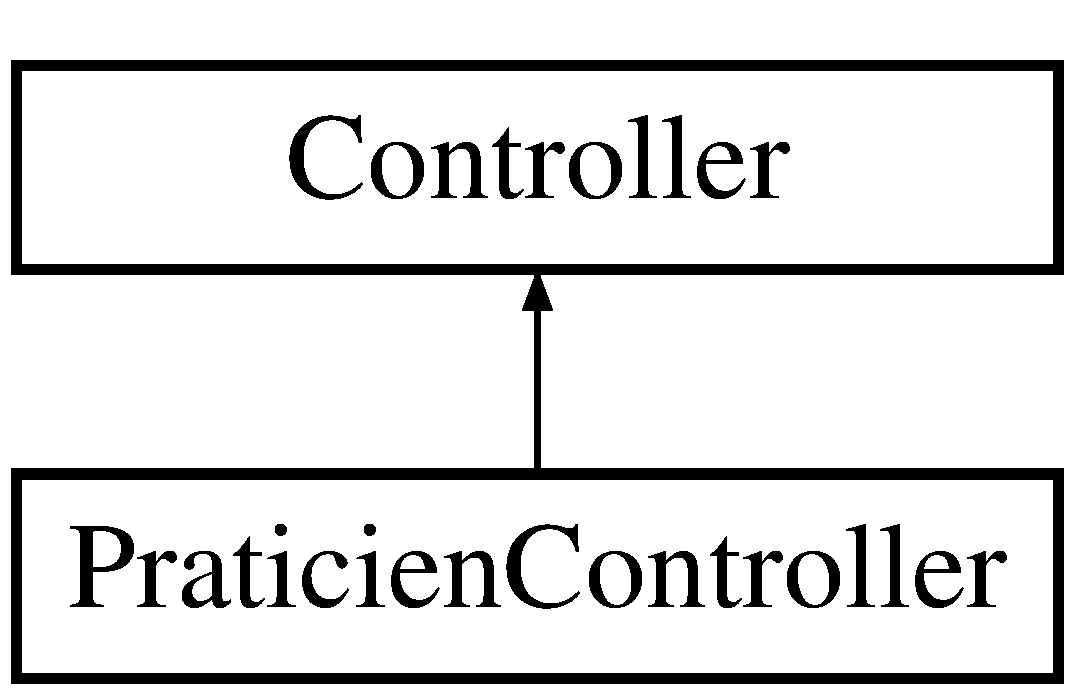
\includegraphics[height=2.000000cm]{class_c_r_1_1_g_s_b_r_bundle_1_1_controller_1_1_praticien_controller}
\end{center}
\end{figure}
\subsection*{Public Member Functions}
\begin{DoxyCompactItemize}
\item 
{\bf index\+Action} ()
\item 
{\bf recherche\+Action} ()
\item 
{\bf recherche\+Avance\+Action} ()
\item 
{\bf resultat\+Action} (Request \$request)
\item 
{\bf resultat\+\_\+avance\+Action} (Request \$request)
\end{DoxyCompactItemize}


\subsection{Detailed Description}
Classe contrôleur de consultation et rechercher des praticiens 

\subsection{Member Function Documentation}
\index{C\+R\+::\+G\+S\+B\+R\+Bundle\+::\+Controller\+::\+Praticien\+Controller@{C\+R\+::\+G\+S\+B\+R\+Bundle\+::\+Controller\+::\+Praticien\+Controller}!index\+Action@{index\+Action}}
\index{index\+Action@{index\+Action}!C\+R\+::\+G\+S\+B\+R\+Bundle\+::\+Controller\+::\+Praticien\+Controller@{C\+R\+::\+G\+S\+B\+R\+Bundle\+::\+Controller\+::\+Praticien\+Controller}}
\subsubsection[{index\+Action}]{\setlength{\rightskip}{0pt plus 5cm}index\+Action (
\begin{DoxyParamCaption}
{}
\end{DoxyParamCaption}
)}\label{class_c_r_1_1_g_s_b_r_bundle_1_1_controller_1_1_praticien_controller_a04f2101fe1cdc785b61219c2df753024}
Cette fonction affiche la page /praticien/ \begin{DoxyReturn}{Returns}
view La vue praticien.\+html.\+twig 
\end{DoxyReturn}
\index{C\+R\+::\+G\+S\+B\+R\+Bundle\+::\+Controller\+::\+Praticien\+Controller@{C\+R\+::\+G\+S\+B\+R\+Bundle\+::\+Controller\+::\+Praticien\+Controller}!recherche\+Action@{recherche\+Action}}
\index{recherche\+Action@{recherche\+Action}!C\+R\+::\+G\+S\+B\+R\+Bundle\+::\+Controller\+::\+Praticien\+Controller@{C\+R\+::\+G\+S\+B\+R\+Bundle\+::\+Controller\+::\+Praticien\+Controller}}
\subsubsection[{recherche\+Action}]{\setlength{\rightskip}{0pt plus 5cm}recherche\+Action (
\begin{DoxyParamCaption}
{}
\end{DoxyParamCaption}
)}\label{class_c_r_1_1_g_s_b_r_bundle_1_1_controller_1_1_praticien_controller_afc5ebc9e38bd370740b7bce95f708232}
Cette fonction recherche l\textquotesingle{}ensemble des praticiens \begin{DoxyReturn}{Returns}
view recherche\+Praticien.\+html.\+twig la vue de recherche de praticiens 
\end{DoxyReturn}
\index{C\+R\+::\+G\+S\+B\+R\+Bundle\+::\+Controller\+::\+Praticien\+Controller@{C\+R\+::\+G\+S\+B\+R\+Bundle\+::\+Controller\+::\+Praticien\+Controller}!recherche\+Avance\+Action@{recherche\+Avance\+Action}}
\index{recherche\+Avance\+Action@{recherche\+Avance\+Action}!C\+R\+::\+G\+S\+B\+R\+Bundle\+::\+Controller\+::\+Praticien\+Controller@{C\+R\+::\+G\+S\+B\+R\+Bundle\+::\+Controller\+::\+Praticien\+Controller}}
\subsubsection[{recherche\+Avance\+Action}]{\setlength{\rightskip}{0pt plus 5cm}recherche\+Avance\+Action (
\begin{DoxyParamCaption}
{}
\end{DoxyParamCaption}
)}\label{class_c_r_1_1_g_s_b_r_bundle_1_1_controller_1_1_praticien_controller_a153c9568b56ae753e7a5939f336ebf40}
Cette fonction recherche l\textquotesingle{}ensemble des praticiens \begin{DoxyReturn}{Returns}
view recherche\+Praticien.\+html.\+twig la vue de recherche avancée de praticiens 
\end{DoxyReturn}
\index{C\+R\+::\+G\+S\+B\+R\+Bundle\+::\+Controller\+::\+Praticien\+Controller@{C\+R\+::\+G\+S\+B\+R\+Bundle\+::\+Controller\+::\+Praticien\+Controller}!resultat\+\_\+avance\+Action@{resultat\+\_\+avance\+Action}}
\index{resultat\+\_\+avance\+Action@{resultat\+\_\+avance\+Action}!C\+R\+::\+G\+S\+B\+R\+Bundle\+::\+Controller\+::\+Praticien\+Controller@{C\+R\+::\+G\+S\+B\+R\+Bundle\+::\+Controller\+::\+Praticien\+Controller}}
\subsubsection[{resultat\+\_\+avance\+Action}]{\setlength{\rightskip}{0pt plus 5cm}resultat\+\_\+avance\+Action (
\begin{DoxyParamCaption}
\item[{Request}]{\$request}
\end{DoxyParamCaption}
)}\label{class_c_r_1_1_g_s_b_r_bundle_1_1_controller_1_1_praticien_controller_aef448f0868eb8382f1be0e1f6805a50a}
Cette fonction retourne le résultat de la recherche avancée de praticiens


\begin{DoxyParams}[1]{Parameters}
Request & {\em \$request} & La requête construite à partir de la séléction de l\textquotesingle{}utilisateur \\
\hline
\end{DoxyParams}
\begin{DoxyReturn}{Returns}
view recherche\+Praticien.\+html.\+twig la vue avec le résultat 
\end{DoxyReturn}
\index{C\+R\+::\+G\+S\+B\+R\+Bundle\+::\+Controller\+::\+Praticien\+Controller@{C\+R\+::\+G\+S\+B\+R\+Bundle\+::\+Controller\+::\+Praticien\+Controller}!resultat\+Action@{resultat\+Action}}
\index{resultat\+Action@{resultat\+Action}!C\+R\+::\+G\+S\+B\+R\+Bundle\+::\+Controller\+::\+Praticien\+Controller@{C\+R\+::\+G\+S\+B\+R\+Bundle\+::\+Controller\+::\+Praticien\+Controller}}
\subsubsection[{resultat\+Action}]{\setlength{\rightskip}{0pt plus 5cm}resultat\+Action (
\begin{DoxyParamCaption}
\item[{Request}]{\$request}
\end{DoxyParamCaption}
)}\label{class_c_r_1_1_g_s_b_r_bundle_1_1_controller_1_1_praticien_controller_a815e9d79cde937c21578a068a15e888f}
Cette fonction retourne le résultat de la recherche de praticien


\begin{DoxyParams}[1]{Parameters}
Request & {\em \$request} & La requête construite à partir de la séléction de l\textquotesingle{}utilisateur \\
\hline
\end{DoxyParams}
\begin{DoxyReturn}{Returns}
view recherche\+Praticien.\+html.\+twig la vue avec le résultat 
\end{DoxyReturn}


The documentation for this class was generated from the following file\+:\begin{DoxyCompactItemize}
\item 
X\+A\+M\+P\+P/xamppfiles/htdocs/\+C\+R/src/\+C\+R/\+G\+S\+B\+R\+Bundle/\+Controller/Praticien\+Controller.\+php\end{DoxyCompactItemize}

\section{praticien\+Repository Class Reference}
\label{class_c_r_1_1_g_s_b_r_bundle_1_1_entity_1_1praticien_repository}\index{praticien\+Repository@{praticien\+Repository}}
Inheritance diagram for praticien\+Repository\+:\begin{figure}[H]
\begin{center}
\leavevmode
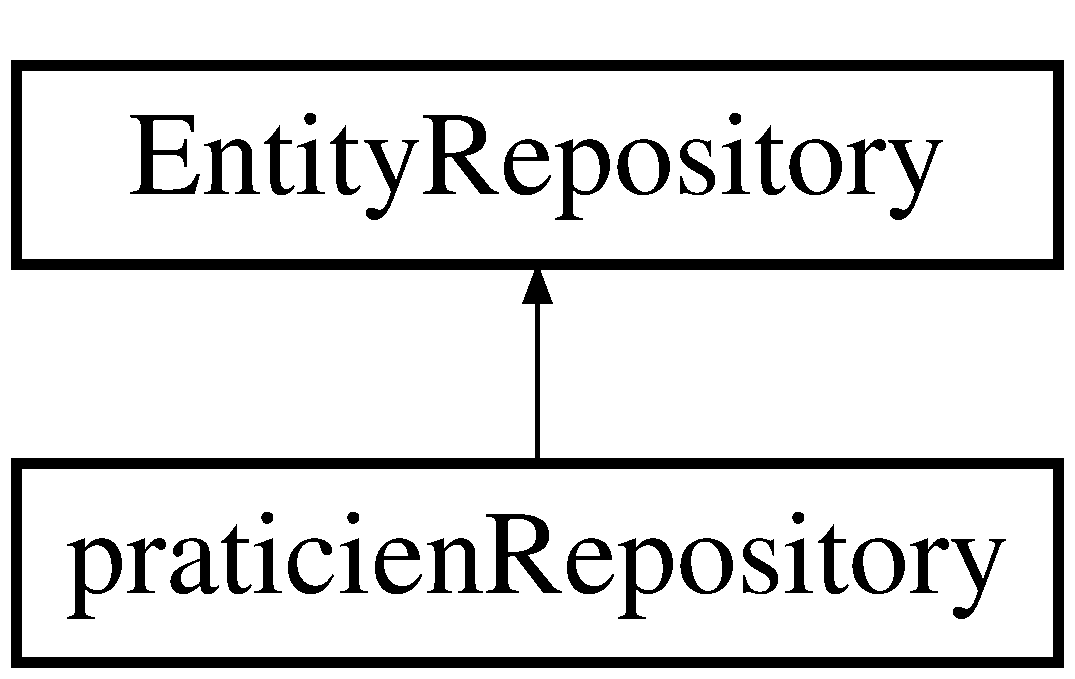
\includegraphics[height=2.000000cm]{class_c_r_1_1_g_s_b_r_bundle_1_1_entity_1_1praticien_repository}
\end{center}
\end{figure}
\subsection*{Public Member Functions}
\begin{DoxyCompactItemize}
\item 
{\bfseries find\+All} ()\label{class_c_r_1_1_g_s_b_r_bundle_1_1_entity_1_1praticien_repository_a73a1b0348919b6755e4f69dcc70eba64}

\end{DoxyCompactItemize}


\subsection{Detailed Description}
\doxyref{praticien\+Repository}{p.}{class_c_r_1_1_g_s_b_r_bundle_1_1_entity_1_1praticien_repository}

This class was generated by the Doctrine O\+R\+M. Add your own custom repository methods below. 

The documentation for this class was generated from the following file\+:\begin{DoxyCompactItemize}
\item 
X\+A\+M\+P\+P/xamppfiles/htdocs/\+C\+R/src/\+C\+R/\+G\+S\+B\+R\+Bundle/\+Entity/praticien\+Repository.\+php\end{DoxyCompactItemize}

\section{rapport\+Visite Class Reference}
\label{class_c_r_1_1_g_s_b_r_bundle_1_1_entity_1_1rapport_visite}\index{rapport\+Visite@{rapport\+Visite}}
\subsection*{Public Member Functions}
\begin{DoxyCompactItemize}
\item 
{\bf get\+Id} ()
\item 
{\bf set\+Date\+Rapport} (\$date\+Rapport)
\item 
{\bf get\+Date\+Rapport} ()
\item 
{\bf set\+Bilan} (\$bilan)
\item 
{\bf get\+Bilan} ()
\item 
{\bf set\+Motif} (\$motif)
\item 
{\bf get\+Motif} ()
\item 
{\bf set\+Visiteur} (\textbackslash{}{\bf C\+R\textbackslash{}\+G\+S\+B\+R\+Bundle\textbackslash{}\+Entity\textbackslash{}visiteur} \${\bf visiteur}=null)
\item 
{\bf get\+Visiteur} ()
\item 
{\bf set\+Medecin} (\textbackslash{}{\bf C\+R\textbackslash{}\+G\+S\+B\+R\+Bundle\textbackslash{}\+Entity\textbackslash{}praticien} \$medecin=null)
\item 
{\bf get\+Medecin} ()
\item 
{\bf is\+Motif\+Valid} (Execution\+Context\+Interface \$context)
\item 
{\bf is\+Bilan\+Valid} (Execution\+Context\+Interface \$context)
\end{DoxyCompactItemize}


\subsection{Detailed Description}
\doxyref{rapport\+Visite}{p.}{class_c_r_1_1_g_s_b_r_bundle_1_1_entity_1_1rapport_visite}

() (repository\+Class=\char`\"{}\+C\+R\textbackslash{}\+G\+S\+B\+R\+Bundle\textbackslash{}\+Entity\textbackslash{}rapport\+Visite\+Repository\char`\"{}) 

\subsection{Member Function Documentation}
\index{C\+R\+::\+G\+S\+B\+R\+Bundle\+::\+Entity\+::rapport\+Visite@{C\+R\+::\+G\+S\+B\+R\+Bundle\+::\+Entity\+::rapport\+Visite}!get\+Bilan@{get\+Bilan}}
\index{get\+Bilan@{get\+Bilan}!C\+R\+::\+G\+S\+B\+R\+Bundle\+::\+Entity\+::rapport\+Visite@{C\+R\+::\+G\+S\+B\+R\+Bundle\+::\+Entity\+::rapport\+Visite}}
\subsubsection[{get\+Bilan}]{\setlength{\rightskip}{0pt plus 5cm}get\+Bilan (
\begin{DoxyParamCaption}
{}
\end{DoxyParamCaption}
)}\label{class_c_r_1_1_g_s_b_r_bundle_1_1_entity_1_1rapport_visite_ace0d83bf5564aa34cd8041d3dbd8857e}
Get bilan

\begin{DoxyReturn}{Returns}
string 
\end{DoxyReturn}
\index{C\+R\+::\+G\+S\+B\+R\+Bundle\+::\+Entity\+::rapport\+Visite@{C\+R\+::\+G\+S\+B\+R\+Bundle\+::\+Entity\+::rapport\+Visite}!get\+Date\+Rapport@{get\+Date\+Rapport}}
\index{get\+Date\+Rapport@{get\+Date\+Rapport}!C\+R\+::\+G\+S\+B\+R\+Bundle\+::\+Entity\+::rapport\+Visite@{C\+R\+::\+G\+S\+B\+R\+Bundle\+::\+Entity\+::rapport\+Visite}}
\subsubsection[{get\+Date\+Rapport}]{\setlength{\rightskip}{0pt plus 5cm}get\+Date\+Rapport (
\begin{DoxyParamCaption}
{}
\end{DoxyParamCaption}
)}\label{class_c_r_1_1_g_s_b_r_bundle_1_1_entity_1_1rapport_visite_a3f155d8d75ea430f0f500b71cdedf61f}
Get date\+Rapport

\begin{DoxyReturn}{Returns}

\end{DoxyReturn}
\index{C\+R\+::\+G\+S\+B\+R\+Bundle\+::\+Entity\+::rapport\+Visite@{C\+R\+::\+G\+S\+B\+R\+Bundle\+::\+Entity\+::rapport\+Visite}!get\+Id@{get\+Id}}
\index{get\+Id@{get\+Id}!C\+R\+::\+G\+S\+B\+R\+Bundle\+::\+Entity\+::rapport\+Visite@{C\+R\+::\+G\+S\+B\+R\+Bundle\+::\+Entity\+::rapport\+Visite}}
\subsubsection[{get\+Id}]{\setlength{\rightskip}{0pt plus 5cm}get\+Id (
\begin{DoxyParamCaption}
{}
\end{DoxyParamCaption}
)}\label{class_c_r_1_1_g_s_b_r_bundle_1_1_entity_1_1rapport_visite_a12251d0c022e9e21c137a105ff683f13}
Get id

\begin{DoxyReturn}{Returns}
integer 
\end{DoxyReturn}
\index{C\+R\+::\+G\+S\+B\+R\+Bundle\+::\+Entity\+::rapport\+Visite@{C\+R\+::\+G\+S\+B\+R\+Bundle\+::\+Entity\+::rapport\+Visite}!get\+Medecin@{get\+Medecin}}
\index{get\+Medecin@{get\+Medecin}!C\+R\+::\+G\+S\+B\+R\+Bundle\+::\+Entity\+::rapport\+Visite@{C\+R\+::\+G\+S\+B\+R\+Bundle\+::\+Entity\+::rapport\+Visite}}
\subsubsection[{get\+Medecin}]{\setlength{\rightskip}{0pt plus 5cm}get\+Medecin (
\begin{DoxyParamCaption}
{}
\end{DoxyParamCaption}
)}\label{class_c_r_1_1_g_s_b_r_bundle_1_1_entity_1_1rapport_visite_a665d645b5e287f2ea898cfd86c4fdfdb}
Get medecin

\begin{DoxyReturn}{Returns}

\end{DoxyReturn}
\index{C\+R\+::\+G\+S\+B\+R\+Bundle\+::\+Entity\+::rapport\+Visite@{C\+R\+::\+G\+S\+B\+R\+Bundle\+::\+Entity\+::rapport\+Visite}!get\+Motif@{get\+Motif}}
\index{get\+Motif@{get\+Motif}!C\+R\+::\+G\+S\+B\+R\+Bundle\+::\+Entity\+::rapport\+Visite@{C\+R\+::\+G\+S\+B\+R\+Bundle\+::\+Entity\+::rapport\+Visite}}
\subsubsection[{get\+Motif}]{\setlength{\rightskip}{0pt plus 5cm}get\+Motif (
\begin{DoxyParamCaption}
{}
\end{DoxyParamCaption}
)}\label{class_c_r_1_1_g_s_b_r_bundle_1_1_entity_1_1rapport_visite_a085fa884d73ecb3b63ee037e8d7ffb25}
Get motif

\begin{DoxyReturn}{Returns}
string 
\end{DoxyReturn}
\index{C\+R\+::\+G\+S\+B\+R\+Bundle\+::\+Entity\+::rapport\+Visite@{C\+R\+::\+G\+S\+B\+R\+Bundle\+::\+Entity\+::rapport\+Visite}!get\+Visiteur@{get\+Visiteur}}
\index{get\+Visiteur@{get\+Visiteur}!C\+R\+::\+G\+S\+B\+R\+Bundle\+::\+Entity\+::rapport\+Visite@{C\+R\+::\+G\+S\+B\+R\+Bundle\+::\+Entity\+::rapport\+Visite}}
\subsubsection[{get\+Visiteur}]{\setlength{\rightskip}{0pt plus 5cm}get\+Visiteur (
\begin{DoxyParamCaption}
{}
\end{DoxyParamCaption}
)}\label{class_c_r_1_1_g_s_b_r_bundle_1_1_entity_1_1rapport_visite_a6f3715343eb260691c71380997c1811f}
Get visiteur

\begin{DoxyReturn}{Returns}

\end{DoxyReturn}
\index{C\+R\+::\+G\+S\+B\+R\+Bundle\+::\+Entity\+::rapport\+Visite@{C\+R\+::\+G\+S\+B\+R\+Bundle\+::\+Entity\+::rapport\+Visite}!is\+Bilan\+Valid@{is\+Bilan\+Valid}}
\index{is\+Bilan\+Valid@{is\+Bilan\+Valid}!C\+R\+::\+G\+S\+B\+R\+Bundle\+::\+Entity\+::rapport\+Visite@{C\+R\+::\+G\+S\+B\+R\+Bundle\+::\+Entity\+::rapport\+Visite}}
\subsubsection[{is\+Bilan\+Valid}]{\setlength{\rightskip}{0pt plus 5cm}is\+Bilan\+Valid (
\begin{DoxyParamCaption}
\item[{Execution\+Context\+Interface}]{\$context}
\end{DoxyParamCaption}
)}\label{class_c_r_1_1_g_s_b_r_bundle_1_1_entity_1_1rapport_visite_ab1cc80762481e5e25dd5591964430ab3}
\index{C\+R\+::\+G\+S\+B\+R\+Bundle\+::\+Entity\+::rapport\+Visite@{C\+R\+::\+G\+S\+B\+R\+Bundle\+::\+Entity\+::rapport\+Visite}!is\+Motif\+Valid@{is\+Motif\+Valid}}
\index{is\+Motif\+Valid@{is\+Motif\+Valid}!C\+R\+::\+G\+S\+B\+R\+Bundle\+::\+Entity\+::rapport\+Visite@{C\+R\+::\+G\+S\+B\+R\+Bundle\+::\+Entity\+::rapport\+Visite}}
\subsubsection[{is\+Motif\+Valid}]{\setlength{\rightskip}{0pt plus 5cm}is\+Motif\+Valid (
\begin{DoxyParamCaption}
\item[{Execution\+Context\+Interface}]{\$context}
\end{DoxyParamCaption}
)}\label{class_c_r_1_1_g_s_b_r_bundle_1_1_entity_1_1rapport_visite_a559e304120dc0c710f57e8cc08a8d6e4}
\index{C\+R\+::\+G\+S\+B\+R\+Bundle\+::\+Entity\+::rapport\+Visite@{C\+R\+::\+G\+S\+B\+R\+Bundle\+::\+Entity\+::rapport\+Visite}!set\+Bilan@{set\+Bilan}}
\index{set\+Bilan@{set\+Bilan}!C\+R\+::\+G\+S\+B\+R\+Bundle\+::\+Entity\+::rapport\+Visite@{C\+R\+::\+G\+S\+B\+R\+Bundle\+::\+Entity\+::rapport\+Visite}}
\subsubsection[{set\+Bilan}]{\setlength{\rightskip}{0pt plus 5cm}set\+Bilan (
\begin{DoxyParamCaption}
\item[{}]{\$bilan}
\end{DoxyParamCaption}
)}\label{class_c_r_1_1_g_s_b_r_bundle_1_1_entity_1_1rapport_visite_ac5cc736e95bae0b51f75fc766cc2e22a}
Set bilan


\begin{DoxyParams}[1]{Parameters}
string & {\em \$bilan} & \\
\hline
\end{DoxyParams}
\begin{DoxyReturn}{Returns}
\doxyref{rapport\+Visite}{p.}{class_c_r_1_1_g_s_b_r_bundle_1_1_entity_1_1rapport_visite} 
\end{DoxyReturn}
\index{C\+R\+::\+G\+S\+B\+R\+Bundle\+::\+Entity\+::rapport\+Visite@{C\+R\+::\+G\+S\+B\+R\+Bundle\+::\+Entity\+::rapport\+Visite}!set\+Date\+Rapport@{set\+Date\+Rapport}}
\index{set\+Date\+Rapport@{set\+Date\+Rapport}!C\+R\+::\+G\+S\+B\+R\+Bundle\+::\+Entity\+::rapport\+Visite@{C\+R\+::\+G\+S\+B\+R\+Bundle\+::\+Entity\+::rapport\+Visite}}
\subsubsection[{set\+Date\+Rapport}]{\setlength{\rightskip}{0pt plus 5cm}set\+Date\+Rapport (
\begin{DoxyParamCaption}
\item[{}]{\$date\+Rapport}
\end{DoxyParamCaption}
)}\label{class_c_r_1_1_g_s_b_r_bundle_1_1_entity_1_1rapport_visite_a4b23bf7af42bafeb96e53383b57a18a4}
Set date\+Rapport


\begin{DoxyParams}[1]{Parameters}
\textbackslash{}\+Date\+Time & {\em \$date\+Rapport} & \\
\hline
\end{DoxyParams}
\begin{DoxyReturn}{Returns}
\doxyref{rapport\+Visite}{p.}{class_c_r_1_1_g_s_b_r_bundle_1_1_entity_1_1rapport_visite} 
\end{DoxyReturn}
\index{C\+R\+::\+G\+S\+B\+R\+Bundle\+::\+Entity\+::rapport\+Visite@{C\+R\+::\+G\+S\+B\+R\+Bundle\+::\+Entity\+::rapport\+Visite}!set\+Medecin@{set\+Medecin}}
\index{set\+Medecin@{set\+Medecin}!C\+R\+::\+G\+S\+B\+R\+Bundle\+::\+Entity\+::rapport\+Visite@{C\+R\+::\+G\+S\+B\+R\+Bundle\+::\+Entity\+::rapport\+Visite}}
\subsubsection[{set\+Medecin}]{\setlength{\rightskip}{0pt plus 5cm}set\+Medecin (
\begin{DoxyParamCaption}
\item[{\textbackslash{}{\bf C\+R\textbackslash{}\+G\+S\+B\+R\+Bundle\textbackslash{}\+Entity\textbackslash{}praticien}}]{\$medecin = {\ttfamily null}}
\end{DoxyParamCaption}
)}\label{class_c_r_1_1_g_s_b_r_bundle_1_1_entity_1_1rapport_visite_ac559ed8dbb5617e214d51854429547a1}
Set medecin


\begin{DoxyParams}[1]{Parameters}
\textbackslash{}\+C\+R\textbackslash{}\+G\+S\+B\+R\+Bundle\textbackslash{}\+Entity\textbackslash{}praticien & {\em \$medecin} & \\
\hline
\end{DoxyParams}
\begin{DoxyReturn}{Returns}
\doxyref{rapport\+Visite}{p.}{class_c_r_1_1_g_s_b_r_bundle_1_1_entity_1_1rapport_visite} 
\end{DoxyReturn}
\index{C\+R\+::\+G\+S\+B\+R\+Bundle\+::\+Entity\+::rapport\+Visite@{C\+R\+::\+G\+S\+B\+R\+Bundle\+::\+Entity\+::rapport\+Visite}!set\+Motif@{set\+Motif}}
\index{set\+Motif@{set\+Motif}!C\+R\+::\+G\+S\+B\+R\+Bundle\+::\+Entity\+::rapport\+Visite@{C\+R\+::\+G\+S\+B\+R\+Bundle\+::\+Entity\+::rapport\+Visite}}
\subsubsection[{set\+Motif}]{\setlength{\rightskip}{0pt plus 5cm}set\+Motif (
\begin{DoxyParamCaption}
\item[{}]{\$motif}
\end{DoxyParamCaption}
)}\label{class_c_r_1_1_g_s_b_r_bundle_1_1_entity_1_1rapport_visite_a76bc256fa2c5eaebbacc0bc1a1f903e9}
Set motif


\begin{DoxyParams}[1]{Parameters}
string & {\em \$motif} & \\
\hline
\end{DoxyParams}
\begin{DoxyReturn}{Returns}
\doxyref{rapport\+Visite}{p.}{class_c_r_1_1_g_s_b_r_bundle_1_1_entity_1_1rapport_visite} 
\end{DoxyReturn}
\index{C\+R\+::\+G\+S\+B\+R\+Bundle\+::\+Entity\+::rapport\+Visite@{C\+R\+::\+G\+S\+B\+R\+Bundle\+::\+Entity\+::rapport\+Visite}!set\+Visiteur@{set\+Visiteur}}
\index{set\+Visiteur@{set\+Visiteur}!C\+R\+::\+G\+S\+B\+R\+Bundle\+::\+Entity\+::rapport\+Visite@{C\+R\+::\+G\+S\+B\+R\+Bundle\+::\+Entity\+::rapport\+Visite}}
\subsubsection[{set\+Visiteur}]{\setlength{\rightskip}{0pt plus 5cm}set\+Visiteur (
\begin{DoxyParamCaption}
\item[{\textbackslash{}{\bf C\+R\textbackslash{}\+G\+S\+B\+R\+Bundle\textbackslash{}\+Entity\textbackslash{}visiteur}}]{\$visiteur = {\ttfamily null}}
\end{DoxyParamCaption}
)}\label{class_c_r_1_1_g_s_b_r_bundle_1_1_entity_1_1rapport_visite_a090aabec3babd8d533c6c3ef5f5843f9}
Set visiteur


\begin{DoxyParams}[1]{Parameters}
\textbackslash{}\+C\+R\textbackslash{}\+G\+S\+B\+R\+Bundle\textbackslash{}\+Entity\textbackslash{}visiteur & {\em \$visiteur} & \\
\hline
\end{DoxyParams}
\begin{DoxyReturn}{Returns}
\doxyref{rapport\+Visite}{p.}{class_c_r_1_1_g_s_b_r_bundle_1_1_entity_1_1rapport_visite} 
\end{DoxyReturn}


The documentation for this class was generated from the following file\+:\begin{DoxyCompactItemize}
\item 
X\+A\+M\+P\+P/xamppfiles/htdocs/\+C\+R/src/\+C\+R/\+G\+S\+B\+R\+Bundle/\+Entity/rapport\+Visite.\+php\end{DoxyCompactItemize}

\section{Rapport\+Visite\+Controller Class Reference}
\label{class_c_r_1_1_g_s_b_r_bundle_1_1_controller_1_1_rapport_visite_controller}\index{Rapport\+Visite\+Controller@{Rapport\+Visite\+Controller}}
Inheritance diagram for Rapport\+Visite\+Controller\+:\begin{figure}[H]
\begin{center}
\leavevmode
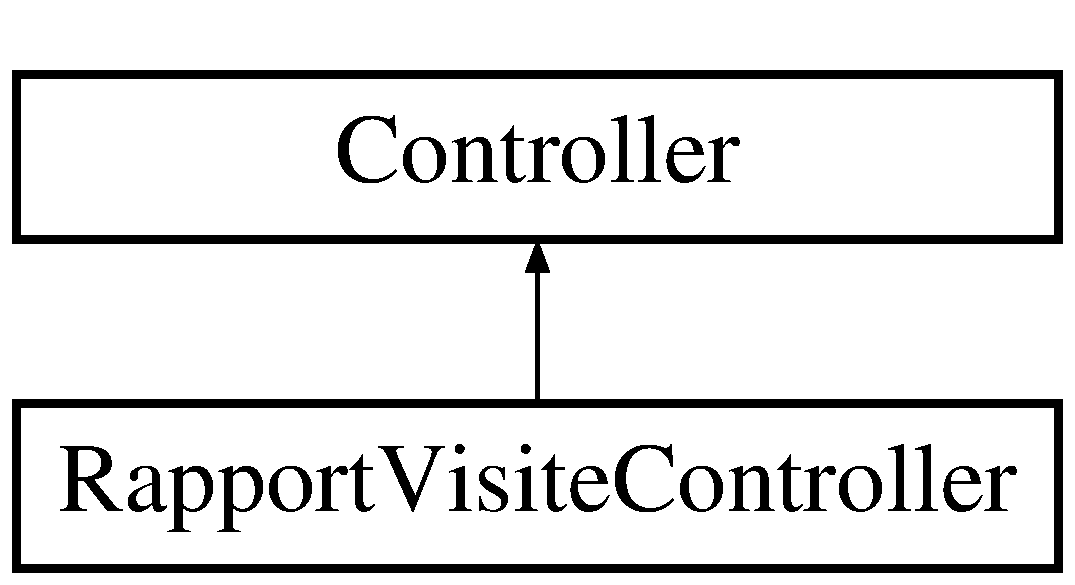
\includegraphics[height=2.000000cm]{class_c_r_1_1_g_s_b_r_bundle_1_1_controller_1_1_rapport_visite_controller}
\end{center}
\end{figure}
\subsection*{Public Member Functions}
\begin{DoxyCompactItemize}
\item 
{\bf index\+Action} ()
\item 
{\bf ajouter\+Action} (Request \$request)
\item 
{\bf supprimer\+Action} (\$id, Request \$request)
\item 
{\bf modifier\+Action} (\$id, Request \$request)
\end{DoxyCompactItemize}


\subsection{Detailed Description}
Classe contrôleur de consultation et de gsetion des rapports de visite 

\subsection{Member Function Documentation}
\index{C\+R\+::\+G\+S\+B\+R\+Bundle\+::\+Controller\+::\+Rapport\+Visite\+Controller@{C\+R\+::\+G\+S\+B\+R\+Bundle\+::\+Controller\+::\+Rapport\+Visite\+Controller}!ajouter\+Action@{ajouter\+Action}}
\index{ajouter\+Action@{ajouter\+Action}!C\+R\+::\+G\+S\+B\+R\+Bundle\+::\+Controller\+::\+Rapport\+Visite\+Controller@{C\+R\+::\+G\+S\+B\+R\+Bundle\+::\+Controller\+::\+Rapport\+Visite\+Controller}}
\subsubsection[{ajouter\+Action}]{\setlength{\rightskip}{0pt plus 5cm}ajouter\+Action (
\begin{DoxyParamCaption}
\item[{Request}]{\$request}
\end{DoxyParamCaption}
)}\label{class_c_r_1_1_g_s_b_r_bundle_1_1_controller_1_1_rapport_visite_controller_a41dd2ddcb78a080e06000141a52a8f21}
Cette fonction ajoute un rapport de visite 
\begin{DoxyParams}[1]{Parameters}
Request & {\em \$request} & La requête construite à partir de la saisie de l\textquotesingle{}utilisateur \\
\hline
\end{DoxyParams}
\begin{DoxyReturn}{Returns}
view la vue ajouter\+Rapport\+Visite.\+html.\+twig 
\end{DoxyReturn}
\index{C\+R\+::\+G\+S\+B\+R\+Bundle\+::\+Controller\+::\+Rapport\+Visite\+Controller@{C\+R\+::\+G\+S\+B\+R\+Bundle\+::\+Controller\+::\+Rapport\+Visite\+Controller}!index\+Action@{index\+Action}}
\index{index\+Action@{index\+Action}!C\+R\+::\+G\+S\+B\+R\+Bundle\+::\+Controller\+::\+Rapport\+Visite\+Controller@{C\+R\+::\+G\+S\+B\+R\+Bundle\+::\+Controller\+::\+Rapport\+Visite\+Controller}}
\subsubsection[{index\+Action}]{\setlength{\rightskip}{0pt plus 5cm}index\+Action (
\begin{DoxyParamCaption}
{}
\end{DoxyParamCaption}
)}\label{class_c_r_1_1_g_s_b_r_bundle_1_1_controller_1_1_rapport_visite_controller_a04f2101fe1cdc785b61219c2df753024}
Cette fonction affiche la page rapport-\/de-\/visite \begin{DoxyReturn}{Returns}
view La vue rapport\+Visite.\+html.\+twig 
\end{DoxyReturn}
\index{C\+R\+::\+G\+S\+B\+R\+Bundle\+::\+Controller\+::\+Rapport\+Visite\+Controller@{C\+R\+::\+G\+S\+B\+R\+Bundle\+::\+Controller\+::\+Rapport\+Visite\+Controller}!modifier\+Action@{modifier\+Action}}
\index{modifier\+Action@{modifier\+Action}!C\+R\+::\+G\+S\+B\+R\+Bundle\+::\+Controller\+::\+Rapport\+Visite\+Controller@{C\+R\+::\+G\+S\+B\+R\+Bundle\+::\+Controller\+::\+Rapport\+Visite\+Controller}}
\subsubsection[{modifier\+Action}]{\setlength{\rightskip}{0pt plus 5cm}modifier\+Action (
\begin{DoxyParamCaption}
\item[{}]{\$id, }
\item[{Request}]{\$request}
\end{DoxyParamCaption}
)}\label{class_c_r_1_1_g_s_b_r_bundle_1_1_controller_1_1_rapport_visite_controller_a57147f9495534a299b833ef500766a79}
Cette fonction modifie un rapport de visite 
\begin{DoxyParams}[1]{Parameters}
int & {\em \$id} & identifiant \\
\hline
Request & {\em \$request} & La requête construite à partir de la saisie de l\textquotesingle{}utilisateur \\
\hline
\end{DoxyParams}
\begin{DoxyReturn}{Returns}
view modifier.\+html.\+twig La vue qui supprime le rapport de visite 
\end{DoxyReturn}
\index{C\+R\+::\+G\+S\+B\+R\+Bundle\+::\+Controller\+::\+Rapport\+Visite\+Controller@{C\+R\+::\+G\+S\+B\+R\+Bundle\+::\+Controller\+::\+Rapport\+Visite\+Controller}!supprimer\+Action@{supprimer\+Action}}
\index{supprimer\+Action@{supprimer\+Action}!C\+R\+::\+G\+S\+B\+R\+Bundle\+::\+Controller\+::\+Rapport\+Visite\+Controller@{C\+R\+::\+G\+S\+B\+R\+Bundle\+::\+Controller\+::\+Rapport\+Visite\+Controller}}
\subsubsection[{supprimer\+Action}]{\setlength{\rightskip}{0pt plus 5cm}supprimer\+Action (
\begin{DoxyParamCaption}
\item[{}]{\$id, }
\item[{Request}]{\$request}
\end{DoxyParamCaption}
)}\label{class_c_r_1_1_g_s_b_r_bundle_1_1_controller_1_1_rapport_visite_controller_a46bf5852619bffc05272889356fd7f63}
Cette fonction supprime un rapport de visite 
\begin{DoxyParams}[1]{Parameters}
int & {\em \$id} & identifiant \\
\hline
Request & {\em \$request} & La requête construite à partir de la saisie de l\textquotesingle{}utilisateur \\
\hline
\end{DoxyParams}
\begin{DoxyReturn}{Returns}
view supprimer.\+html.\+twig La vue qui supprime le rapport de visite 
\end{DoxyReturn}


The documentation for this class was generated from the following file\+:\begin{DoxyCompactItemize}
\item 
X\+A\+M\+P\+P/xamppfiles/htdocs/\+C\+R/src/\+C\+R/\+G\+S\+B\+R\+Bundle/\+Controller/Rapport\+Visite\+Controller.\+php\end{DoxyCompactItemize}

\section{rapport\+Visite\+Repository Class Reference}
\label{class_c_r_1_1_g_s_b_r_bundle_1_1_entity_1_1rapport_visite_repository}\index{rapport\+Visite\+Repository@{rapport\+Visite\+Repository}}
Inheritance diagram for rapport\+Visite\+Repository\+:\begin{figure}[H]
\begin{center}
\leavevmode
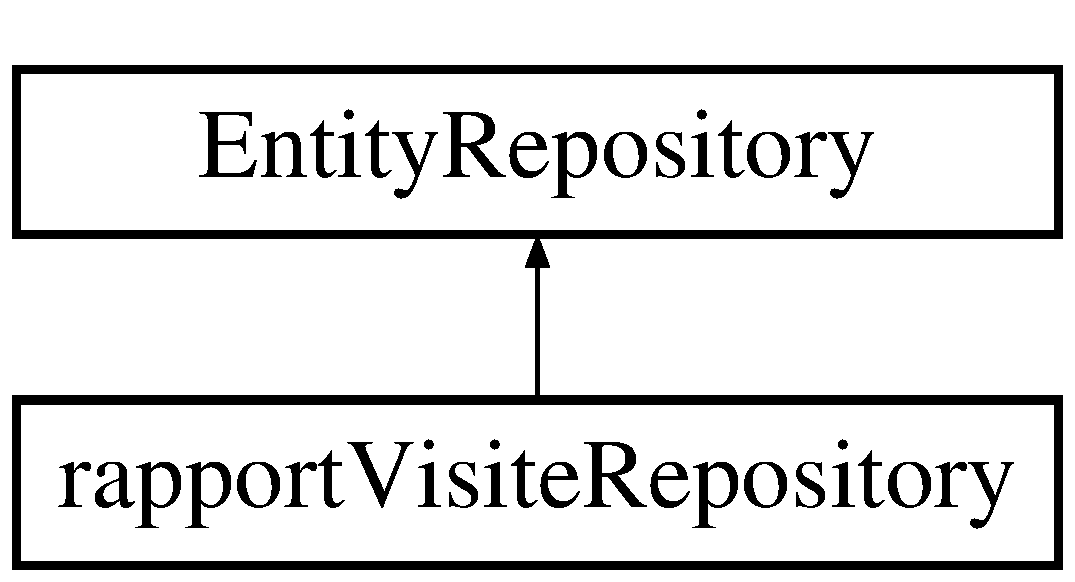
\includegraphics[height=2.000000cm]{class_c_r_1_1_g_s_b_r_bundle_1_1_entity_1_1rapport_visite_repository}
\end{center}
\end{figure}


\subsection{Detailed Description}
\doxyref{rapport\+Visite\+Repository}{p.}{class_c_r_1_1_g_s_b_r_bundle_1_1_entity_1_1rapport_visite_repository}

This class was generated by the Doctrine O\+R\+M. Add your own custom repository methods below. 

The documentation for this class was generated from the following file\+:\begin{DoxyCompactItemize}
\item 
X\+A\+M\+P\+P/xamppfiles/htdocs/\+C\+R/src/\+C\+R/\+G\+S\+B\+R\+Bundle/\+Entity/rapport\+Visite\+Repository.\+php\end{DoxyCompactItemize}

\section{type\+Praticien Class Reference}
\label{class_c_r_1_1_g_s_b_r_bundle_1_1_entity_1_1type_praticien}\index{type\+Praticien@{type\+Praticien}}
\subsection*{Public Member Functions}
\begin{DoxyCompactItemize}
\item 
{\bf get\+Id} ()
\item 
{\bf set\+Libelle\+Type} (\$libelle\+Type)
\item 
{\bf get\+Libelle\+Type} ()
\end{DoxyCompactItemize}


\subsection{Detailed Description}
\doxyref{type\+Praticien}{p.}{class_c_r_1_1_g_s_b_r_bundle_1_1_entity_1_1type_praticien}

() (repository\+Class=\char`\"{}\+C\+R\textbackslash{}\+G\+S\+B\+R\+Bundle\textbackslash{}\+Entity\textbackslash{}type\+Praticien\+Repository\char`\"{}) 

\subsection{Member Function Documentation}
\index{C\+R\+::\+G\+S\+B\+R\+Bundle\+::\+Entity\+::type\+Praticien@{C\+R\+::\+G\+S\+B\+R\+Bundle\+::\+Entity\+::type\+Praticien}!get\+Id@{get\+Id}}
\index{get\+Id@{get\+Id}!C\+R\+::\+G\+S\+B\+R\+Bundle\+::\+Entity\+::type\+Praticien@{C\+R\+::\+G\+S\+B\+R\+Bundle\+::\+Entity\+::type\+Praticien}}
\subsubsection[{get\+Id}]{\setlength{\rightskip}{0pt plus 5cm}get\+Id (
\begin{DoxyParamCaption}
{}
\end{DoxyParamCaption}
)}\label{class_c_r_1_1_g_s_b_r_bundle_1_1_entity_1_1type_praticien_a12251d0c022e9e21c137a105ff683f13}
Get id

\begin{DoxyReturn}{Returns}
integer 
\end{DoxyReturn}
\index{C\+R\+::\+G\+S\+B\+R\+Bundle\+::\+Entity\+::type\+Praticien@{C\+R\+::\+G\+S\+B\+R\+Bundle\+::\+Entity\+::type\+Praticien}!get\+Libelle\+Type@{get\+Libelle\+Type}}
\index{get\+Libelle\+Type@{get\+Libelle\+Type}!C\+R\+::\+G\+S\+B\+R\+Bundle\+::\+Entity\+::type\+Praticien@{C\+R\+::\+G\+S\+B\+R\+Bundle\+::\+Entity\+::type\+Praticien}}
\subsubsection[{get\+Libelle\+Type}]{\setlength{\rightskip}{0pt plus 5cm}get\+Libelle\+Type (
\begin{DoxyParamCaption}
{}
\end{DoxyParamCaption}
)}\label{class_c_r_1_1_g_s_b_r_bundle_1_1_entity_1_1type_praticien_a20fe83814f336334af288c1ad4c403be}
Get libelle\+Type

\begin{DoxyReturn}{Returns}
string 
\end{DoxyReturn}
\index{C\+R\+::\+G\+S\+B\+R\+Bundle\+::\+Entity\+::type\+Praticien@{C\+R\+::\+G\+S\+B\+R\+Bundle\+::\+Entity\+::type\+Praticien}!set\+Libelle\+Type@{set\+Libelle\+Type}}
\index{set\+Libelle\+Type@{set\+Libelle\+Type}!C\+R\+::\+G\+S\+B\+R\+Bundle\+::\+Entity\+::type\+Praticien@{C\+R\+::\+G\+S\+B\+R\+Bundle\+::\+Entity\+::type\+Praticien}}
\subsubsection[{set\+Libelle\+Type}]{\setlength{\rightskip}{0pt plus 5cm}set\+Libelle\+Type (
\begin{DoxyParamCaption}
\item[{}]{\$libelle\+Type}
\end{DoxyParamCaption}
)}\label{class_c_r_1_1_g_s_b_r_bundle_1_1_entity_1_1type_praticien_aac5069dd44d16a213d6ff75721b030d1}
Set libelle\+Type


\begin{DoxyParams}[1]{Parameters}
string & {\em \$libelle\+Type} & \\
\hline
\end{DoxyParams}
\begin{DoxyReturn}{Returns}
\doxyref{type\+Praticien}{p.}{class_c_r_1_1_g_s_b_r_bundle_1_1_entity_1_1type_praticien} 
\end{DoxyReturn}


The documentation for this class was generated from the following file\+:\begin{DoxyCompactItemize}
\item 
X\+A\+M\+P\+P/xamppfiles/htdocs/\+C\+R/src/\+C\+R/\+G\+S\+B\+R\+Bundle/\+Entity/type\+Praticien.\+php\end{DoxyCompactItemize}

\section{type\+Praticien\+Repository Class Reference}
\label{class_c_r_1_1_g_s_b_r_bundle_1_1_entity_1_1type_praticien_repository}\index{type\+Praticien\+Repository@{type\+Praticien\+Repository}}
Inheritance diagram for type\+Praticien\+Repository\+:\begin{figure}[H]
\begin{center}
\leavevmode
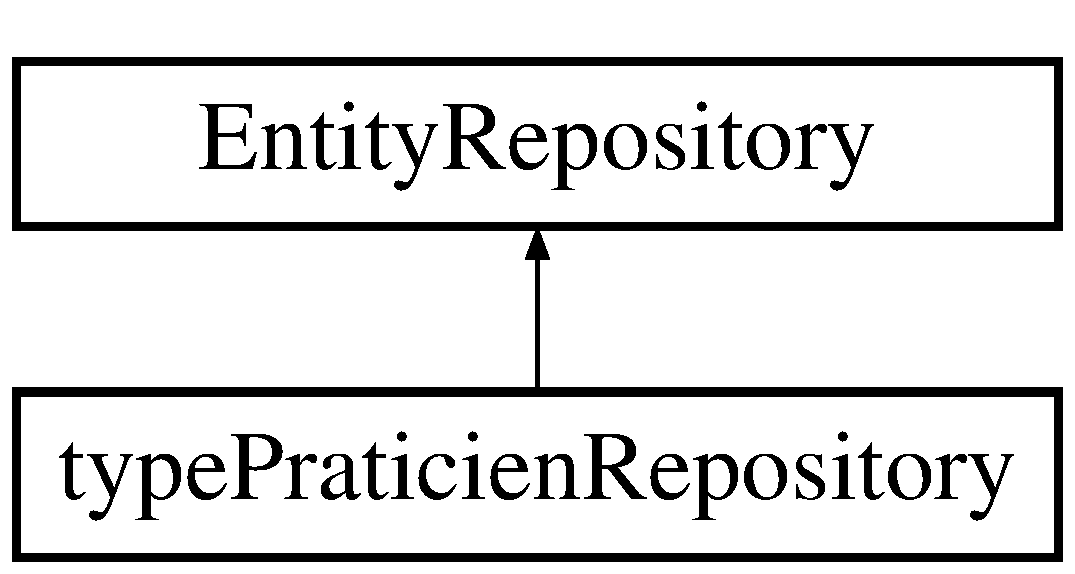
\includegraphics[height=2.000000cm]{class_c_r_1_1_g_s_b_r_bundle_1_1_entity_1_1type_praticien_repository}
\end{center}
\end{figure}
\subsection*{Public Member Functions}
\begin{DoxyCompactItemize}
\item 
{\bfseries find\+All} ()\label{class_c_r_1_1_g_s_b_r_bundle_1_1_entity_1_1type_praticien_repository_a73a1b0348919b6755e4f69dcc70eba64}

\end{DoxyCompactItemize}


\subsection{Detailed Description}
\doxyref{type\+Praticien\+Repository}{p.}{class_c_r_1_1_g_s_b_r_bundle_1_1_entity_1_1type_praticien_repository}

This class was generated by the Doctrine O\+R\+M. Add your own custom repository methods below. 

The documentation for this class was generated from the following file\+:\begin{DoxyCompactItemize}
\item 
X\+A\+M\+P\+P/xamppfiles/htdocs/\+C\+R/src/\+C\+R/\+G\+S\+B\+R\+Bundle/\+Entity/type\+Praticien\+Repository.\+php\end{DoxyCompactItemize}

\section{visiteur Class Reference}
\label{class_c_r_1_1_g_s_b_r_bundle_1_1_entity_1_1visiteur}\index{visiteur@{visiteur}}
Inheritance diagram for visiteur\+:\begin{figure}[H]
\begin{center}
\leavevmode
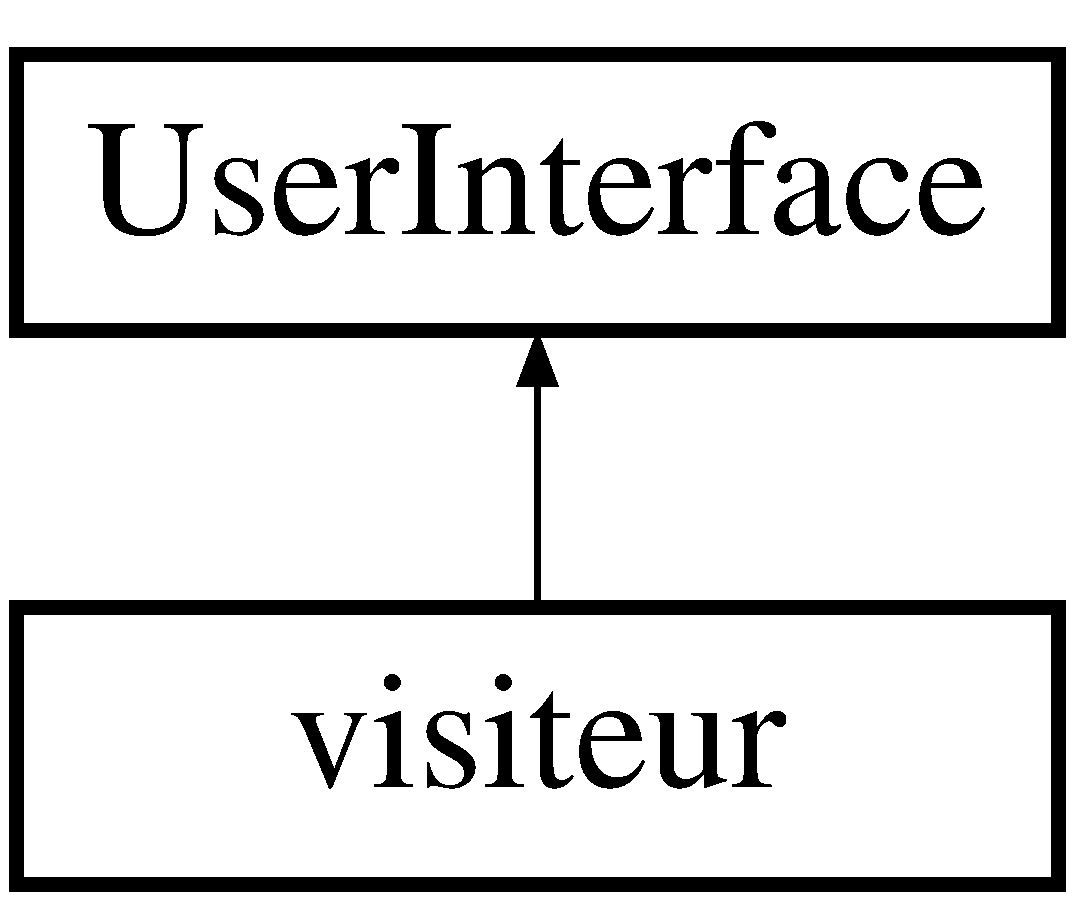
\includegraphics[height=2.000000cm]{class_c_r_1_1_g_s_b_r_bundle_1_1_entity_1_1visiteur}
\end{center}
\end{figure}
\subsection*{Public Member Functions}
\begin{DoxyCompactItemize}
\item 
{\bf get\+Id} ()
\item 
{\bf set\+Id\+G\+S\+B} (\$id\+G\+S\+B)
\item 
{\bf get\+Id\+G\+S\+B} ()
\item 
{\bf set\+Nom} (\$nom)
\item 
{\bf get\+Nom} ()
\item 
{\bf set\+Prenom} (\$prenom)
\item 
{\bf get\+Prenom} ()
\item 
{\bf set\+Username} (\$login)
\item 
{\bf get\+Username} ()
\item 
{\bf set\+Password} (\$mdp)
\item 
{\bf get\+Password} ()
\item 
{\bfseries get\+Mdp} ()\label{class_c_r_1_1_g_s_b_r_bundle_1_1_entity_1_1visiteur_a9cb89ad7e39143daa21704f565df0ff5}

\item 
{\bf set\+Adresse} (\$adresse)
\item 
{\bf get\+Adresse} ()
\item 
{\bf set\+Cp} (\$cp)
\item 
{\bf get\+Cp} ()
\item 
{\bf set\+Ville} (\$ville)
\item 
{\bf get\+Ville} ()
\item 
{\bf set\+Date\+Embauche} (\$date\+Embauche)
\item 
{\bf get\+Date\+Embauche} ()
\item 
{\bfseries erase\+Credentials} ()\label{class_c_r_1_1_g_s_b_r_bundle_1_1_entity_1_1visiteur_ac565b8c00fe93ce673f8237849f072a6}

\item 
{\bfseries get\+Roles} ()\label{class_c_r_1_1_g_s_b_r_bundle_1_1_entity_1_1visiteur_aa676cae5ee8d7fb6862a8724adc2660d}

\item 
{\bfseries get\+Salt} ()\label{class_c_r_1_1_g_s_b_r_bundle_1_1_entity_1_1visiteur_a1dfe56d2c965d451a135f3f3910a8b8d}

\end{DoxyCompactItemize}


\subsection{Detailed Description}
visiteur

() (repository\+Class=\char`\"{}\+C\+R\textbackslash{}\+G\+S\+B\+R\+Bundle\textbackslash{}\+Entity\textbackslash{}visiteur\+Repository\char`\"{}) (fields=\char`\"{}login\char`\"{}, message=\char`\"{}\+Un login similaire existe déjà.\char`\"{}) 

\subsection{Member Function Documentation}
\index{C\+R\+::\+G\+S\+B\+R\+Bundle\+::\+Entity\+::visiteur@{C\+R\+::\+G\+S\+B\+R\+Bundle\+::\+Entity\+::visiteur}!get\+Adresse@{get\+Adresse}}
\index{get\+Adresse@{get\+Adresse}!C\+R\+::\+G\+S\+B\+R\+Bundle\+::\+Entity\+::visiteur@{C\+R\+::\+G\+S\+B\+R\+Bundle\+::\+Entity\+::visiteur}}
\subsubsection[{get\+Adresse}]{\setlength{\rightskip}{0pt plus 5cm}get\+Adresse (
\begin{DoxyParamCaption}
{}
\end{DoxyParamCaption}
)}\label{class_c_r_1_1_g_s_b_r_bundle_1_1_entity_1_1visiteur_a1c3323aa9b0c805f3ed4aec98142d326}
Get adresse

\begin{DoxyReturn}{Returns}
string 
\end{DoxyReturn}
\index{C\+R\+::\+G\+S\+B\+R\+Bundle\+::\+Entity\+::visiteur@{C\+R\+::\+G\+S\+B\+R\+Bundle\+::\+Entity\+::visiteur}!get\+Cp@{get\+Cp}}
\index{get\+Cp@{get\+Cp}!C\+R\+::\+G\+S\+B\+R\+Bundle\+::\+Entity\+::visiteur@{C\+R\+::\+G\+S\+B\+R\+Bundle\+::\+Entity\+::visiteur}}
\subsubsection[{get\+Cp}]{\setlength{\rightskip}{0pt plus 5cm}get\+Cp (
\begin{DoxyParamCaption}
{}
\end{DoxyParamCaption}
)}\label{class_c_r_1_1_g_s_b_r_bundle_1_1_entity_1_1visiteur_a8c5e85bc0648c9752b112794765c2fb2}
Get cp

\begin{DoxyReturn}{Returns}
string 
\end{DoxyReturn}
\index{C\+R\+::\+G\+S\+B\+R\+Bundle\+::\+Entity\+::visiteur@{C\+R\+::\+G\+S\+B\+R\+Bundle\+::\+Entity\+::visiteur}!get\+Date\+Embauche@{get\+Date\+Embauche}}
\index{get\+Date\+Embauche@{get\+Date\+Embauche}!C\+R\+::\+G\+S\+B\+R\+Bundle\+::\+Entity\+::visiteur@{C\+R\+::\+G\+S\+B\+R\+Bundle\+::\+Entity\+::visiteur}}
\subsubsection[{get\+Date\+Embauche}]{\setlength{\rightskip}{0pt plus 5cm}get\+Date\+Embauche (
\begin{DoxyParamCaption}
{}
\end{DoxyParamCaption}
)}\label{class_c_r_1_1_g_s_b_r_bundle_1_1_entity_1_1visiteur_aadf6aac58195a312252da453607788a4}
Get date\+Embauche

\begin{DoxyReturn}{Returns}

\end{DoxyReturn}
\index{C\+R\+::\+G\+S\+B\+R\+Bundle\+::\+Entity\+::visiteur@{C\+R\+::\+G\+S\+B\+R\+Bundle\+::\+Entity\+::visiteur}!get\+Id@{get\+Id}}
\index{get\+Id@{get\+Id}!C\+R\+::\+G\+S\+B\+R\+Bundle\+::\+Entity\+::visiteur@{C\+R\+::\+G\+S\+B\+R\+Bundle\+::\+Entity\+::visiteur}}
\subsubsection[{get\+Id}]{\setlength{\rightskip}{0pt plus 5cm}get\+Id (
\begin{DoxyParamCaption}
{}
\end{DoxyParamCaption}
)}\label{class_c_r_1_1_g_s_b_r_bundle_1_1_entity_1_1visiteur_a12251d0c022e9e21c137a105ff683f13}
Get id

\begin{DoxyReturn}{Returns}
integer 
\end{DoxyReturn}
\index{C\+R\+::\+G\+S\+B\+R\+Bundle\+::\+Entity\+::visiteur@{C\+R\+::\+G\+S\+B\+R\+Bundle\+::\+Entity\+::visiteur}!get\+Id\+G\+S\+B@{get\+Id\+G\+S\+B}}
\index{get\+Id\+G\+S\+B@{get\+Id\+G\+S\+B}!C\+R\+::\+G\+S\+B\+R\+Bundle\+::\+Entity\+::visiteur@{C\+R\+::\+G\+S\+B\+R\+Bundle\+::\+Entity\+::visiteur}}
\subsubsection[{get\+Id\+G\+S\+B}]{\setlength{\rightskip}{0pt plus 5cm}get\+Id\+G\+S\+B (
\begin{DoxyParamCaption}
{}
\end{DoxyParamCaption}
)}\label{class_c_r_1_1_g_s_b_r_bundle_1_1_entity_1_1visiteur_a255464b3339242038a2624e14c92aef0}
Get id\+G\+S\+B

\begin{DoxyReturn}{Returns}
string 
\end{DoxyReturn}
\index{C\+R\+::\+G\+S\+B\+R\+Bundle\+::\+Entity\+::visiteur@{C\+R\+::\+G\+S\+B\+R\+Bundle\+::\+Entity\+::visiteur}!get\+Nom@{get\+Nom}}
\index{get\+Nom@{get\+Nom}!C\+R\+::\+G\+S\+B\+R\+Bundle\+::\+Entity\+::visiteur@{C\+R\+::\+G\+S\+B\+R\+Bundle\+::\+Entity\+::visiteur}}
\subsubsection[{get\+Nom}]{\setlength{\rightskip}{0pt plus 5cm}get\+Nom (
\begin{DoxyParamCaption}
{}
\end{DoxyParamCaption}
)}\label{class_c_r_1_1_g_s_b_r_bundle_1_1_entity_1_1visiteur_a184f2299ee4553fa0782ea87c9aed362}
Get nom

\begin{DoxyReturn}{Returns}
string 
\end{DoxyReturn}
\index{C\+R\+::\+G\+S\+B\+R\+Bundle\+::\+Entity\+::visiteur@{C\+R\+::\+G\+S\+B\+R\+Bundle\+::\+Entity\+::visiteur}!get\+Password@{get\+Password}}
\index{get\+Password@{get\+Password}!C\+R\+::\+G\+S\+B\+R\+Bundle\+::\+Entity\+::visiteur@{C\+R\+::\+G\+S\+B\+R\+Bundle\+::\+Entity\+::visiteur}}
\subsubsection[{get\+Password}]{\setlength{\rightskip}{0pt plus 5cm}get\+Password (
\begin{DoxyParamCaption}
{}
\end{DoxyParamCaption}
)}\label{class_c_r_1_1_g_s_b_r_bundle_1_1_entity_1_1visiteur_a04e0957baeb7acde9c0c86556da2d43f}
Get mdp

\begin{DoxyReturn}{Returns}
string 
\end{DoxyReturn}
\index{C\+R\+::\+G\+S\+B\+R\+Bundle\+::\+Entity\+::visiteur@{C\+R\+::\+G\+S\+B\+R\+Bundle\+::\+Entity\+::visiteur}!get\+Prenom@{get\+Prenom}}
\index{get\+Prenom@{get\+Prenom}!C\+R\+::\+G\+S\+B\+R\+Bundle\+::\+Entity\+::visiteur@{C\+R\+::\+G\+S\+B\+R\+Bundle\+::\+Entity\+::visiteur}}
\subsubsection[{get\+Prenom}]{\setlength{\rightskip}{0pt plus 5cm}get\+Prenom (
\begin{DoxyParamCaption}
{}
\end{DoxyParamCaption}
)}\label{class_c_r_1_1_g_s_b_r_bundle_1_1_entity_1_1visiteur_a2a243ff78ccebcd417fd644325f44701}
Get prenom

\begin{DoxyReturn}{Returns}
string 
\end{DoxyReturn}
\index{C\+R\+::\+G\+S\+B\+R\+Bundle\+::\+Entity\+::visiteur@{C\+R\+::\+G\+S\+B\+R\+Bundle\+::\+Entity\+::visiteur}!get\+Username@{get\+Username}}
\index{get\+Username@{get\+Username}!C\+R\+::\+G\+S\+B\+R\+Bundle\+::\+Entity\+::visiteur@{C\+R\+::\+G\+S\+B\+R\+Bundle\+::\+Entity\+::visiteur}}
\subsubsection[{get\+Username}]{\setlength{\rightskip}{0pt plus 5cm}get\+Username (
\begin{DoxyParamCaption}
{}
\end{DoxyParamCaption}
)}\label{class_c_r_1_1_g_s_b_r_bundle_1_1_entity_1_1visiteur_a81b37a3c9d639574e394f80c1138c75e}
Get login

\begin{DoxyReturn}{Returns}
string 
\end{DoxyReturn}
\index{C\+R\+::\+G\+S\+B\+R\+Bundle\+::\+Entity\+::visiteur@{C\+R\+::\+G\+S\+B\+R\+Bundle\+::\+Entity\+::visiteur}!get\+Ville@{get\+Ville}}
\index{get\+Ville@{get\+Ville}!C\+R\+::\+G\+S\+B\+R\+Bundle\+::\+Entity\+::visiteur@{C\+R\+::\+G\+S\+B\+R\+Bundle\+::\+Entity\+::visiteur}}
\subsubsection[{get\+Ville}]{\setlength{\rightskip}{0pt plus 5cm}get\+Ville (
\begin{DoxyParamCaption}
{}
\end{DoxyParamCaption}
)}\label{class_c_r_1_1_g_s_b_r_bundle_1_1_entity_1_1visiteur_a5fdb46906b99db60cdc126d6e3c606c0}
Get ville

\begin{DoxyReturn}{Returns}
string 
\end{DoxyReturn}
\index{C\+R\+::\+G\+S\+B\+R\+Bundle\+::\+Entity\+::visiteur@{C\+R\+::\+G\+S\+B\+R\+Bundle\+::\+Entity\+::visiteur}!set\+Adresse@{set\+Adresse}}
\index{set\+Adresse@{set\+Adresse}!C\+R\+::\+G\+S\+B\+R\+Bundle\+::\+Entity\+::visiteur@{C\+R\+::\+G\+S\+B\+R\+Bundle\+::\+Entity\+::visiteur}}
\subsubsection[{set\+Adresse}]{\setlength{\rightskip}{0pt plus 5cm}set\+Adresse (
\begin{DoxyParamCaption}
\item[{}]{\$adresse}
\end{DoxyParamCaption}
)}\label{class_c_r_1_1_g_s_b_r_bundle_1_1_entity_1_1visiteur_a0c73311e0d6edc23076eebfd3a100ef4}
Set adresse


\begin{DoxyParams}[1]{Parameters}
string & {\em \$adresse} & \\
\hline
\end{DoxyParams}
\begin{DoxyReturn}{Returns}
visiteur 
\end{DoxyReturn}
\index{C\+R\+::\+G\+S\+B\+R\+Bundle\+::\+Entity\+::visiteur@{C\+R\+::\+G\+S\+B\+R\+Bundle\+::\+Entity\+::visiteur}!set\+Cp@{set\+Cp}}
\index{set\+Cp@{set\+Cp}!C\+R\+::\+G\+S\+B\+R\+Bundle\+::\+Entity\+::visiteur@{C\+R\+::\+G\+S\+B\+R\+Bundle\+::\+Entity\+::visiteur}}
\subsubsection[{set\+Cp}]{\setlength{\rightskip}{0pt plus 5cm}set\+Cp (
\begin{DoxyParamCaption}
\item[{}]{\$cp}
\end{DoxyParamCaption}
)}\label{class_c_r_1_1_g_s_b_r_bundle_1_1_entity_1_1visiteur_ab2f2f5a46713ef0a130b38d4cabf5a9c}
Set cp


\begin{DoxyParams}[1]{Parameters}
string & {\em \$cp} & \\
\hline
\end{DoxyParams}
\begin{DoxyReturn}{Returns}
visiteur 
\end{DoxyReturn}
\index{C\+R\+::\+G\+S\+B\+R\+Bundle\+::\+Entity\+::visiteur@{C\+R\+::\+G\+S\+B\+R\+Bundle\+::\+Entity\+::visiteur}!set\+Date\+Embauche@{set\+Date\+Embauche}}
\index{set\+Date\+Embauche@{set\+Date\+Embauche}!C\+R\+::\+G\+S\+B\+R\+Bundle\+::\+Entity\+::visiteur@{C\+R\+::\+G\+S\+B\+R\+Bundle\+::\+Entity\+::visiteur}}
\subsubsection[{set\+Date\+Embauche}]{\setlength{\rightskip}{0pt plus 5cm}set\+Date\+Embauche (
\begin{DoxyParamCaption}
\item[{}]{\$date\+Embauche}
\end{DoxyParamCaption}
)}\label{class_c_r_1_1_g_s_b_r_bundle_1_1_entity_1_1visiteur_ad09a21c47cc96e31455ddbf1166059fc}
Set date\+Embauche


\begin{DoxyParams}[1]{Parameters}
\textbackslash{}\+Date\+Time & {\em \$date\+Embauche} & \\
\hline
\end{DoxyParams}
\begin{DoxyReturn}{Returns}
visiteur 
\end{DoxyReturn}
\index{C\+R\+::\+G\+S\+B\+R\+Bundle\+::\+Entity\+::visiteur@{C\+R\+::\+G\+S\+B\+R\+Bundle\+::\+Entity\+::visiteur}!set\+Id\+G\+S\+B@{set\+Id\+G\+S\+B}}
\index{set\+Id\+G\+S\+B@{set\+Id\+G\+S\+B}!C\+R\+::\+G\+S\+B\+R\+Bundle\+::\+Entity\+::visiteur@{C\+R\+::\+G\+S\+B\+R\+Bundle\+::\+Entity\+::visiteur}}
\subsubsection[{set\+Id\+G\+S\+B}]{\setlength{\rightskip}{0pt plus 5cm}set\+Id\+G\+S\+B (
\begin{DoxyParamCaption}
\item[{}]{\$id\+G\+S\+B}
\end{DoxyParamCaption}
)}\label{class_c_r_1_1_g_s_b_r_bundle_1_1_entity_1_1visiteur_a2201812d8e699d67c5177564124f483d}
Set id\+G\+S\+B


\begin{DoxyParams}[1]{Parameters}
string & {\em \$id\+G\+S\+B} & \\
\hline
\end{DoxyParams}
\begin{DoxyReturn}{Returns}
visiteur 
\end{DoxyReturn}
\index{C\+R\+::\+G\+S\+B\+R\+Bundle\+::\+Entity\+::visiteur@{C\+R\+::\+G\+S\+B\+R\+Bundle\+::\+Entity\+::visiteur}!set\+Nom@{set\+Nom}}
\index{set\+Nom@{set\+Nom}!C\+R\+::\+G\+S\+B\+R\+Bundle\+::\+Entity\+::visiteur@{C\+R\+::\+G\+S\+B\+R\+Bundle\+::\+Entity\+::visiteur}}
\subsubsection[{set\+Nom}]{\setlength{\rightskip}{0pt plus 5cm}set\+Nom (
\begin{DoxyParamCaption}
\item[{}]{\$nom}
\end{DoxyParamCaption}
)}\label{class_c_r_1_1_g_s_b_r_bundle_1_1_entity_1_1visiteur_a3c162f28ffbb9c8026c0d84f722e5060}
Set nom


\begin{DoxyParams}[1]{Parameters}
string & {\em \$nom} & \\
\hline
\end{DoxyParams}
\begin{DoxyReturn}{Returns}
visiteur 
\end{DoxyReturn}
\index{C\+R\+::\+G\+S\+B\+R\+Bundle\+::\+Entity\+::visiteur@{C\+R\+::\+G\+S\+B\+R\+Bundle\+::\+Entity\+::visiteur}!set\+Password@{set\+Password}}
\index{set\+Password@{set\+Password}!C\+R\+::\+G\+S\+B\+R\+Bundle\+::\+Entity\+::visiteur@{C\+R\+::\+G\+S\+B\+R\+Bundle\+::\+Entity\+::visiteur}}
\subsubsection[{set\+Password}]{\setlength{\rightskip}{0pt plus 5cm}set\+Password (
\begin{DoxyParamCaption}
\item[{}]{\$mdp}
\end{DoxyParamCaption}
)}\label{class_c_r_1_1_g_s_b_r_bundle_1_1_entity_1_1visiteur_aab4b61e5788ec8b289a3c540cd78da9f}
Set mdp


\begin{DoxyParams}[1]{Parameters}
string & {\em \$mdp} & \\
\hline
\end{DoxyParams}
\begin{DoxyReturn}{Returns}
visiteur 
\end{DoxyReturn}
\index{C\+R\+::\+G\+S\+B\+R\+Bundle\+::\+Entity\+::visiteur@{C\+R\+::\+G\+S\+B\+R\+Bundle\+::\+Entity\+::visiteur}!set\+Prenom@{set\+Prenom}}
\index{set\+Prenom@{set\+Prenom}!C\+R\+::\+G\+S\+B\+R\+Bundle\+::\+Entity\+::visiteur@{C\+R\+::\+G\+S\+B\+R\+Bundle\+::\+Entity\+::visiteur}}
\subsubsection[{set\+Prenom}]{\setlength{\rightskip}{0pt plus 5cm}set\+Prenom (
\begin{DoxyParamCaption}
\item[{}]{\$prenom}
\end{DoxyParamCaption}
)}\label{class_c_r_1_1_g_s_b_r_bundle_1_1_entity_1_1visiteur_aab06d96cb012bde67fdbf4f8bfdad2a8}
Set prenom


\begin{DoxyParams}[1]{Parameters}
string & {\em \$prenom} & \\
\hline
\end{DoxyParams}
\begin{DoxyReturn}{Returns}
visiteur 
\end{DoxyReturn}
\index{C\+R\+::\+G\+S\+B\+R\+Bundle\+::\+Entity\+::visiteur@{C\+R\+::\+G\+S\+B\+R\+Bundle\+::\+Entity\+::visiteur}!set\+Username@{set\+Username}}
\index{set\+Username@{set\+Username}!C\+R\+::\+G\+S\+B\+R\+Bundle\+::\+Entity\+::visiteur@{C\+R\+::\+G\+S\+B\+R\+Bundle\+::\+Entity\+::visiteur}}
\subsubsection[{set\+Username}]{\setlength{\rightskip}{0pt plus 5cm}set\+Username (
\begin{DoxyParamCaption}
\item[{}]{\$login}
\end{DoxyParamCaption}
)}\label{class_c_r_1_1_g_s_b_r_bundle_1_1_entity_1_1visiteur_aa11072e203a300f9774edd2cea830261}
Set login


\begin{DoxyParams}[1]{Parameters}
string & {\em \$login} & \\
\hline
\end{DoxyParams}
\begin{DoxyReturn}{Returns}
visiteur 
\end{DoxyReturn}
\index{C\+R\+::\+G\+S\+B\+R\+Bundle\+::\+Entity\+::visiteur@{C\+R\+::\+G\+S\+B\+R\+Bundle\+::\+Entity\+::visiteur}!set\+Ville@{set\+Ville}}
\index{set\+Ville@{set\+Ville}!C\+R\+::\+G\+S\+B\+R\+Bundle\+::\+Entity\+::visiteur@{C\+R\+::\+G\+S\+B\+R\+Bundle\+::\+Entity\+::visiteur}}
\subsubsection[{set\+Ville}]{\setlength{\rightskip}{0pt plus 5cm}set\+Ville (
\begin{DoxyParamCaption}
\item[{}]{\$ville}
\end{DoxyParamCaption}
)}\label{class_c_r_1_1_g_s_b_r_bundle_1_1_entity_1_1visiteur_a0b029761e53c7225a87f08cf47ad2b49}
Set ville


\begin{DoxyParams}[1]{Parameters}
string & {\em \$ville} & \\
\hline
\end{DoxyParams}
\begin{DoxyReturn}{Returns}
visiteur 
\end{DoxyReturn}


The documentation for this class was generated from the following file\+:\begin{DoxyCompactItemize}
\item 
X\+A\+M\+P\+P/xamppfiles/htdocs/\+C\+R/src/\+C\+R/\+G\+S\+B\+R\+Bundle/\+Entity/visiteur.\+php\end{DoxyCompactItemize}

\section{visiteur\+Repository Class Reference}
\label{class_c_r_1_1_g_s_b_r_bundle_1_1_entity_1_1visiteur_repository}\index{visiteur\+Repository@{visiteur\+Repository}}
Inheritance diagram for visiteur\+Repository\+:\begin{figure}[H]
\begin{center}
\leavevmode
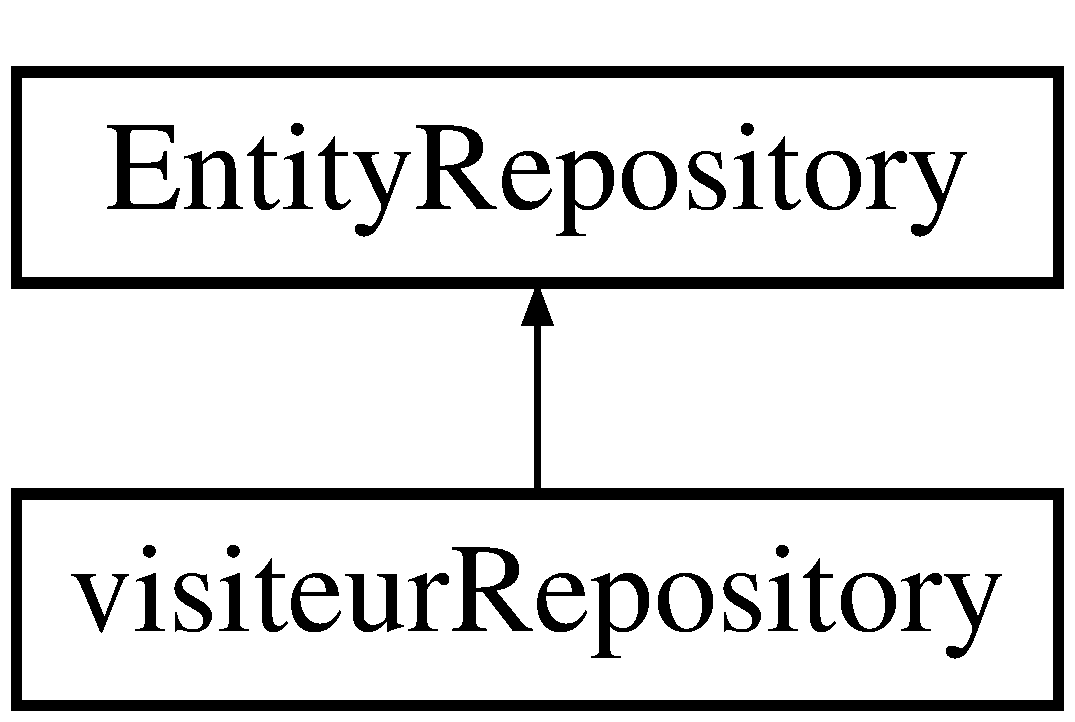
\includegraphics[height=2.000000cm]{class_c_r_1_1_g_s_b_r_bundle_1_1_entity_1_1visiteur_repository}
\end{center}
\end{figure}
\subsection*{Public Member Functions}
\begin{DoxyCompactItemize}
\item 
{\bfseries find\+Visiteur} (\$login, \$mdp)\label{class_c_r_1_1_g_s_b_r_bundle_1_1_entity_1_1visiteur_repository_ad2f233df3f4ce54858434a0324324fa0}

\end{DoxyCompactItemize}


\subsection{Detailed Description}
\doxyref{visiteur\+Repository}{p.}{class_c_r_1_1_g_s_b_r_bundle_1_1_entity_1_1visiteur_repository}

This class was generated by the Doctrine O\+R\+M. Add your own custom repository methods below. 

The documentation for this class was generated from the following file\+:\begin{DoxyCompactItemize}
\item 
X\+A\+M\+P\+P/xamppfiles/htdocs/\+C\+R/src/\+C\+R/\+G\+S\+B\+R\+Bundle/\+Entity/visiteur\+Repository.\+php\end{DoxyCompactItemize}

%--- End generated contents ---

% Index
\backmatter
\newpage
\phantomsection
\clearemptydoublepage
\addcontentsline{toc}{chapter}{Index}
\printindex

\end{document}
